\documentclass[fleqn,reqno,10pt]{article}


\usepackage[natbib=true,
            style=authoryear-comp,
            backend=bibtex,
            sortcites=false,
            maxnames=2,
            doi=false,
            url=false]{biblatex}
\bibliography{MyRefGlobal}
% \bibliography{paper}

\usepackage[final,            % override "draft" which means "no nothing"
            colorlinks,       % rather than outlining them in boxes
            linkcolor=gray,   % override truly awful color choices
            citecolor=gray,   %   (ditto)
            urlcolor=gray,    %   (ditto)
            plainpages=false, % to overcome complaints with multiple
            pdfpagelabels,    % multiple page 1-s due to preface
            hypertexnames=false % solves warning, but interferes with
                                % index and \autoref apparently
            ]{hyperref}


\usepackage{amsmath}            % Formeln
\usepackage{amsfonts}           % Fonts for Formulas
\usepackage{amssymb}
\usepackage[final]{graphicx}
\usepackage{booktabs}
\usepackage{enumerate}
\usepackage{lipsum}
\usepackage{txfonts} % for strict implication symbols
\usepackage{soul}
\usepackage{relsize} % provides command \relsize{+/-x} for relative
                     % font size changes
\usepackage[german,english]{babel}
\usepackage[utf8]{inputenc}
\usepackage[T1]{fontenc} 
\usepackage{subfig}
\usepackage{xypic}
\usepackage{url}
\usepackage{tikz}
\usetikzlibrary{arrows,shapes,automata,backgrounds,petri,fit,decorations.pathmorphing}
\usepackage{refcount}
\usepackage{xspace} % for \xspace in definition of acronyms etc.
\usepackage{attrib} % for right-aligned references at the end of
                    % quotes; part of Frankenstein bundle, but 
\renewcommand\PreTrib {}   % overwrite these commands, from attrib.sty
\renewcommand\PostTrib {}  % to suppress additional brackets around
                           % attributions
\usepackage{eurosym}
\usepackage{pgfplots}
\usepackage{todonotes}

\usepackage{gb4e_micha}


\usepackage{mycommands}

% \usepackage{geometry}
% \linespread{1.2}

%%%% Additional Macros

\newcommand{\lit}{\acro{lit}}
\newcommand{\glb}{\acro{glb}}
\newcommand{\loc}{\acro{loc}}

\newcommand{\as}{\acro{as}}
\renewcommand{\es}{\acro{es}}
\renewcommand{\AE}{\as}
\newcommand{\GE}{\es}
\newcommand{\ea}{\acro{ea}}

\newcommand{\lc}{\acro{lc}}
\newcommand{\ec}{\acro{ec}}
\newcommand{\LC}{\lc}
\newcommand{\EC}{\ec}

\newcommand{\exh}{\ensuremath{\mathrm{Exh}}}
\newcommand{\alt}{\ensuremath{\mathrm{Alt}}}

\newcommand{\ivt}{\acro{ivt}}

\renewcommand{\mymark}[1]{\textbf{#1}}

\pgfplotscreateplotcyclelist{mylist}{% 
    {solid,black},
    {dotted,black}, 
    {dashed,black}, 
    {loosely dotted,gray}, 
    {solid,black},
    {dotted,black},
    {dashed,black},
    {loosely dotted}}

\usetikzlibrary{calc}
\usepackage{nicefrac}

%%%% Document

\title{Embedded Scalars, Preferred Readings \& Prosody: {A}n
  Experimental Revisit} 
\author{% Michael Franke, Fabian Schlotterbeck and Petra Augurzky
} 
\date{}

\begin{document}
\maketitle



\begin{abstract}
  The scalar item \emph{some} is widely assumed to receive a meaning
  enrichment to \emph{some but not all} if it occurs in matrix
  position. The question under which circumstances this enrichment can
  occur in certain embedded positions plays an important role in
  deciding how to delineate semantics and pragmatics. % Some claim
  % that it requires marked intonation for the relevant pragmatic
  % enrichment to occur in embedded position; others allow for it more
  % freely.
  We present new experimental data that bear on this theoretical issue. In distinction to
  previous experimental approaches, we presented sentence material auditorily in order to
  explicitly control prosodic markedness of the scalar item. Moreover, our experiment sheds
  light on the relative preferences or salience of candidate readings. The presented data turn
  out to be unexpected under a traditional Gricean view, but also challenge the idea that of
  disambiguation by logical strength in grammaticalist approaches.
\end{abstract}




\section{Introduction}
\label{sec:introduction}

The existential quantifier \emph{some} is usually assumed to receive a
semantic interpretation similar to logical $\exists$, so that
(\ref{bsp:Plain-SI-Target}) is literally true even when Hans solved
all of the problems. But use of \emph{some} is also usually considered
to invite comparison with (at least) the semantically stronger
universal quantifier \emph{all}
\citep[c.f.][]{Horn1972:On-the-Semantic,Gazdar1979:Pragmatics:-Imp,AtlasLevinson1981}. This
scalar comparison can lead to an upper-bound meaning enrichment, e.g.,
when an utterance of (\ref{bsp:Plain-SI-Target}) is taken to invite
the inference in (\ref{bsp:Plain-SI-Implicature}).

\begin{exe}
  \ex \label{bsp:Plain-SI}
    \begin{xlist}
      \ex \label{bsp:Plain-SI-Target} Hans solved some of the
        problems.
      \ex \label{bsp:Plain-SI-Implicature} $\implicates$ Hans solved
        some but not all of the problems.
      \ex \label{bsp:Plain-SI-Alternative} Hans solved all of the problems.
    \end{xlist}
\end{exe}

\noindent The classical explanation of this inference, following the
pioneering work of \citet{Grice1975:Logic-and-Conve}, is that
(\ref{bsp:Plain-SI-Implicature}) is a pragmatic inference, a so-called
\emph{quantity implicature}, derived by an abductive inference to the
best explanation of why informed, knowledgable and cooperative
speakers would utter (\ref{bsp:Plain-SI-Target}) when they could also
utter the semantically stronger and relevant
(\ref{bsp:Plain-SI-Alternative}) \citep[see][for a recent
overview]{Geurts2010:Quantity-Implic}.


% If this upper-bound inference would occur often and
% systematically enough, then it may well be that also embedded
% occurrences of \emph{some} get enriched, in some fashion or other, to
% contribute the enriched meaning \emph{some but not all} also under the
% scope of other logical operators.
% Indeed, even
% \citeauthor{Grice1975:Logic-and-Conve} envisaged this possibility when
% he wrote: ``It may not be impossible for what starts life, so to
% speak, as a conversational implicature to become conventionalized''
% \citep[p.58]{Grice1975:Logic-and-Conve}.

Whereas the existence of such implicatures is rather uncontroversial
for plain occurrences of \emph{some}, it is still an issue of debate
whether comparable enrichments are also found in so-called
``embedded'' cases, where the scalar item \emph{some} occurs in the
scope of other logical operators. This paper deals with two such
cases.  In \as-sentences (mnemonic for \textit{all \dots some \dots})
as in (\ref{bsp:AE}) the scalar item \emph{some} is embedded under the
universal quantifier \emph{all}. In \es-sentences (mnemonic for
\textit{exactly one \dots some \dots}) like (\ref{bsp:GE}) \emph{some}
takes scope under the non-monotonic quantifier \emph{exactly one}.
Current theories, have proposed at least three candidate readings for
\as- and \es-sentences: (i) a \emph{literal reading} like in
(\ref{bsp:AE-Literal}) and (\ref{bsp:GE-Literal}) where \emph{some}
has only its literal meaning; (ii) a \emph{global reading} like in
(\ref{bsp:AE-Global}) and (\ref{bsp:GE-Global}) where the meaning of
(\ref{bsp:AE}) and (\ref{bsp:GE}) is enriched with the negation of the
corresponding sentences (\ref{bsp:AE-Alternative}) and
(\ref{bsp:GE-Alternative}) respectively; and also (iii) a \emph{local
  reading} like in (\ref{bsp:AE-Local}) and (\ref{bsp:GE-Local}) where
\emph{some} is interpreted as \emph{some but not all} in the scope of
the embedding quantifier.

\begin{exe}
  \ex \label{bsp:AE} \mymark{All} of the students read {\mymark{some}} of the
  papers. \hfill{(\as)}

  \begin{xlist}
  \ex \label{bsp:AE-Literal} \mymark{All} of the students read
    {\mymark{some and maybe all}} of the papers. \hfill (\as-\lit)
  \ex \label{bsp:AE-Global}
    \mymark{All} of the students read \mymark{some and maybe all} 
    and  \hfill (\as-\glb)\\
    it's not the case that \mymark{all} of the students read \mymark{all} of the papers.
  \ex \label{bsp:AE-Local}
    \mymark{All} of the students read {\mymark{some  but not all}} of the
    papers. \hfill (\as-\loc)
  \end{xlist}
\end{exe}

\begin{exe}
\ex  \label{bsp:GE} \mymark{Exactly one} of the students read {\mymark{some}} of the
  papers. \hfill{(\es)}

  \begin{xlist}
  \ex \label{bsp:GE-Literal} \mymark{Exactly one} of the students read
    {\mymark{some and maybe all}} of the papers. \hfill (\es-\lit)
  \ex \label{bsp:GE-Global}
    \mymark{Exactly one} of the students read \mymark{some and maybe all} 
    and  \hfill (\es-\glb)\\
    it's not the case that \mymark{exactly one} of the students read \mymark{all} of the papers.
  \ex \label{bsp:GE-Local}
    \mymark{Exactly one} of the students read {\mymark{some  but not all}} of the
    papers. \hfill (\es-\loc)
  \end{xlist}
\end{exe}


\begin{exe}
\ex \label{bsp:AE-Alternative} \mymark{All} of the students read
  {\mymark{all}} of the papers. 

\ex \label{bsp:GE-Alternative} \mymark{Exactly one} of the students
  read {\mymark{all}} of the papers.
\end{exe}

Given this plurality of hypothesized readings, the question arises:
how \emph{salient} are these theoretically conceivable readings compared to
each other, or, put differently, what is the \emph{preference order} on
hypothesized readings (if they are detectable by empirical means at all)?
Addressing this question empirically is relevant because it lies at
the heart of a current debate about the nature of quantity inferences.
The controversy is usually seen as one between two main competing
theoretical positions, which we call \emph{traditionalism} and
\emph{grammaticalism} and take to be general ideas behind large
classes of approaches to quantity implicatures \citep[c.f.][for related
discussion with a focus on deriving processing
theories]{ChemlaSingh2014:Remarks-on-the-}. % Unfortunately, it is
% rather difficult to empirically test either ``core theory''
% (terminology from \citeauthor{ChemlaSingh2014:Remarks-on-the-})
% directly because additional ``auxiliary assumptions'' are needed to
% derive falsifiable \emph{ex ante} predictions about to-be-expected
% observations in a concrete behavioral experiment, even irrespective of
% processing accounts. We therefore try to carefully set up plausible
% instantiations of either core theory with particular auxiliary
% assumptions that give testable predictions at the outset in
% Section~\ref{sec:theories-predictions}, then evaluate the obtained
% predictions against our data, and finally broaden our perspective to
% reflect in Section~\ref{sec:critical-reflection} on the impact of our
% data on the more general tenability of the core theories.

Results from previous empirical studies have been discussed
controversially
\citep[e.g.][]{GeurtsPouscoulous2009:Embedded-Implic,CliftonDube2010:Embedded-Implic,ChemlaSpector2010:Experimental-Ev,BenzGotzner2014:Embedded-implic}. This
is because of several reasons. Firstly, and most importantly, previous
studies presented target sentences visually.  However, traditionalists
often acknowledge the availability of local readings for prosodically
marked utterances
\citep[e.g.][]{Horn2006:The-Border-Wars,Geurts2009:Scalar-Implicat,ChemlaSpector2010:Experimental-Ev,Geurts2010:Quantity-Implic,Tielvan-Tiel2012:Embedded-Scalar,GeurtsTielvan-Tiel2013:Embedded-Scalar}. Under
this view, evidence for the availability of local readings
\citep[see][]{CliftonDube2010:Embedded-Implic,ChemlaSpector2010:Experimental-Ev}
may be an effect of “silent prosody” \citep[see
e.g.][]{Bader98,Fodor98}. We therefore address this position as the
\emph{prosodic markedness hypothesis} explicitly. Secondly, as
\citet{Tielvan-Tiel2012:Embedded-Scalar} and
\citet{GeurtsTielvan-Tiel2013:Embedded-Scalar} argue, the alleged
evidence for the availability of local readings of \as-sentences,
might well be confounded with, in particular, “typicality effects”
(see Section~\ref{sec:previous-studies} for discussion).  Finally,
previous studies have only accumulated limited evidence pertaining to
the relative salience of candidate readings of sentences like
(\ref{bsp:AE}) and (\ref{bsp:GE}) (see
Section~\ref{sec:previous-studies} for discussion).

% More generally, two prerequisites have to be met in order to make
% use of experimental data to decide between theoretical positions
% regarding the computation of quantity inferences. Firstly, both
% traditionalism and grammaticalism have to be augmented with
% additional assumptions to derive testable predictions about the
% relative salience of candidate readings. For example, hypothezised
% effects of prosodic marking have to be taken into account before we
% can test traditionalism empirically using sentences (\ref{bsp:AE})
% and (\ref{bsp:GE}).  We will address this position as the
% \mymark{prosodic markedness hypothesis} and argue that, if prosody
% is hypothesized to play a central role, it is vital to present
% target sentences auditorily or to control for effects of “silent
% prosody” that subjects may apply when reading a sentence. Secondly,
% the relative salience of candidate readings has to be
% operationalized properly, i.e., we have to devise methods to measure
% relative salience. For example, typicality effects and logical
% dependencies between readings have to be controlled for when
% evaluating speaker judgments in terms of the salience of candidate
% readings.  Both of these prerequisites are related to formulating
% what \citet{ChemlaSingh2014:Remarks-on-the-} call ``auxiliary
% assumptions'' that are necessary to enable theoretical accounts to
% make predictions about processing. Our emphasis here is not on
% processing accounts, but on predictions of behavioral data --- what
% is sometimes, perhaps misleadingly, called a computational-level
% perspective. But even so, traditionalism and grammaticalism have to
% summon auxiliary assumptions which connect the core theories to the
% dependent variables of a behavioral experiment. Without proper
% auxiliary assumptions it is hard (or impossible) to test
% traditionalism or grammaticalism empirically.

To deal with the problem of ``silent intonation,'' this paper presents results from an
experimental study which presented sentence materials auditorily and explicitly manipulated
contrastive stress on embedded scalar items. To address worries about pictorial ``typicality
effects,'' we employed an \emph{incremental verification task} in which parts of a
to-be-evaluated picture were hidden and only revealed piece-wise at the participants’ request
until they felt able to give a binary truth-value judgement \citep[see][]{Conroy2008}. In order
to obtain information about salience of readings, we use both a classical regression analysis
and a Bayesian statistical model to analyze the data from this novel task, and validate this
method by including control conditions testing ambiguous sentences with a well-known preference
on available readings. % We argue that this method provides categorical behavioral data that is
% both indicative of the reading preferences among participants and largely independent of
% potential pictorial confounds, such as the mentioned typicality effects.

% The data obtained by this method is \emph{prima facie} problematic for
% both traditionalism and grammaticalism, at least if augmented by the
% auxiliary assumptions which we adopted here. However, we want to
% stress from the outset that, while the experimental results allow us
% to derive restrictions on which auxiliary assumptions are conceivable
% for traditionalism and grammaticalism, definite conclusions about the
% general validity of the two core theories will be limited
% \citep[cf.][]{ChemlaSingh2014:Remarks-on-the-}. Bearing this in mind,
% we can summarize our main findings crudely as follows. Contrary to the
% predictions of common versions of traditionalism, we observed many
% answers indicative of local readings of \es-sentences, irrespective of
% prosodic markedness. But also prominent versions of grammaticalism are
% incongruent with the observed data.  Backed up by the
% \mymark{strongest meaning hypothesis}
% \citep{DalrympleKanazawa1998:Reciprocal-Expr} as a disambiguation
% criterion \citep[as suggested by][]{ChierchiaFox2008:The-Grammatical},
% grammaticalism predicts local readings to be much more salient than we
% found evidence for in our data. More strongly even, the preference
% order among putative readings suggested by our data cannot even in
% principle be explained by comparisons of logical strength among
% putative readings. This finding is independently relevant in the light
% of the fact that the strongest meaning hypothesis is frequently
% summoned as a disambiguation criterion also in other domains, such as
% the interpretation of reciprocals
% \citep{DalrympleKanazawa1998:Reciprocal-Expr} or vague predicates
% \citep{CobrerosEgre2012:Tolerant-Classi}. In sum, our data shed doubt
% on both traditionalism and grammaticalism under prominent auxiliary
% assumptions. We conclude the paper by some thoughts on how either
% position could be amended in the light of our data.


The paper is structured as follows. Section~\ref{sec:get-know-your}
elaborates on the three kinds of relevant readings for our target
sentences. Section~\ref{sec:theories-predictions} works out testable
\emph{ex ante} predictions of \emph{traditionalism} and
\emph{grammaticalism}. Section~\ref{sec:previous-studies} reviews
related experimental studies to the extent necessary to motivate our
own approach. Section~\ref{sec:exp} describes our experimental design,
analyses and results. Finally, Section~\ref{sec:critical-reflection}
discusses our method and interpretation of the results in a broader
theoretical context.

\section{Get to know your readings}
\label{sec:get-know-your}

Three readings are \emph{prima facie} conceivable for the \as- and
\es-sentences in (\ref{bsp:AE}) and (\ref{bsp:GE}). These are
logically dependent in intricate ways.

\paragraph{\as-sentences.}

An \as-sentence like (\ref{bsp:AE}), repeated below, has a literal
reading (\lit) as in (\ref{bsp:AE-Literal}), a global reading (\glb)
as paraphrased in (\ref{bsp:AE-Global}) and a local reading (\loc) as
in (\ref{bsp:AE-Local}).

\begin{exer}{bsp:AE}

  \ex \mymark{All} of the students read {\mymark{some}} of the
  papers. 

  \begin{xlist}
  \ex \mymark{All} of the students read
    {\mymark{some and maybe all}} of the papers. \hfill (\as-\lit)
  \ex
    \mymark{All} of the students read \mymark{some and maybe all} 
    and  \hfill (\as-\glb)\\
    it's not the case that \mymark{all} of the students read \mymark{all} of the papers.
  \ex
    \mymark{All} of the students read {\mymark{some  but not all}} of the
    papers. \hfill (\as-\loc)
  \end{xlist}
\end{exer}

\noindent These readings stand in a strict entailment relation: the
local reading asymmetrically entails the global reading, which
asymmetrically entails the literal reading:
\begin{exe}
  \ex \label{bsp:Entailments-AS} \loc $\subset$ \glb $\subset$ \lit
\end{exe}
\glb entails \lit because, in general, global readings are defined as
the conjunction of the literal reading and the negated
(relevant/feasible) alternative(s) of the to-be-interpreted
utterance. This entailment is asymmetric, because the information that
not all of the students read all of the papers is not entailed by the
literal reading. To see that \loc $\subset$ \glb, notice that the case
where all of the students read some but not all of the papers is a
special case of the class of situations where all of the students read
some (and maybe all), while not all of the students read all of the
papers.

Given these entailment relations, there are four kinds of situations,
the names for which we borrow from
\citet{ChemlaSpector2010:Experimental-Ev}, that we can distinguish
based on different truth values for our candidate readings. These are
given in Table~\ref{fig:situations-AE}.
%
\begin{table}
  \centering
  \subfloat[][\as-sentences]{
  \label{fig:situations-AE}
    \begin{tabular}{lccc}
    \toprule
    situation    & \multicolumn{3}{c}{reading} 
  \\ 
  \cmidrule(r){2-4}
     & \lit & \glb & \loc \\ \midrule
    false   & 0 & 0 & 0 \\
    literal & 1 & 0 & 0 \\
    weak    & 1 & 1 & 0 \\
    strong  & 1 & 1 & 1 \\ \bottomrule
  \end{tabular}
} \qquad \qquad
  \subfloat[][\es-sentences]{
  \label{fig:situations-GS}
  \begin{tabular}{lccc}
    \toprule
    situation    & \multicolumn{3}{c}{reading} 
  \\ 
  \cmidrule(r){2-4}
    & \textsc{lit} & \textsc{glb} & \textsc{loc} \\ \midrule
    false   & 0 & 0 & 0 \\
    literal & 1 & 0 & 0 \\
    local   & 0 & 0 & 1 \\
    all     & 1 & 1 & 1 \\ \bottomrule
  \end{tabular}
}
\caption{Possible truth-value distributions for readings of \as- and \es-sentences}
\label{tab:situations}
\end{table}
%
Examples of these kinds of situations are shown in
Figure~\ref{fig:AS-distinguishing-pics}, where the dots on the right
of each diagram represent students, the dots on the left represent
papers and an arrow from a student to a paper indicates that the
student read the paper. % Notice that other arrangements of arrows might
% equally well serve as examples for the various situations.

\begin{figure}[t]
  \centering
  
\subfloat[fig:false][false]{
  \label{fig:false-AE}
  
\begin{tikzpicture}[node distance = 1cm]
        % Nodes

        \node (X-1) {$\Large{\bullet}$};

        \node (X-2) [below of = X-1] {$\Large{\bullet}$};

        \node (X-3) [below of = X-2] {$\Large{\bullet}$};

        \node (Y-1) [right of = X-1, node distance = 2cm]{$\Large{\bullet}$};

        \node (Y-2) [below of = Y-1] {$\Large{\bullet}$};

        \node (Y-3) [below of = Y-2] {$\Large{\bullet}$};

        \node (Y-4) [below of = Y-3] {$\Large{\bullet}$};

        % table added from here

        \node (X-4) [below of = X-3, node distance = 2cm] {};

        \node (table) [right of = X-4] {
          \begin{tabular}{ll}
            \lit & false \\
            \glb & false \\
            \loc & false 
          \end{tabular}};

        % Arrows

        \path [draw=blue,->] (X-1) -> (Y-1);

        \path [draw=blue,->] (X-1) -> (Y-2);


        \path [draw=red,->] (X-3) -> (Y-3);

        \path [draw=red,->] (X-3) -> (Y-4);

      \end{tikzpicture}

}
\subfloat[fig:literal][literal]{
  \label{fig:literal-AE}

  \begin{tikzpicture}[node distance = 1cm]
        % Nodes

        \node (X-1) {$\Large{\bullet}$};

        \node (X-2) [below of = X-1] {$\Large{\bullet}$};

        \node (X-3) [below of = X-2] {$\Large{\bullet}$};

        \node (Y-1) [right of = X-1, node distance = 2cm]{$\Large{\bullet}$};

        \node (Y-2) [below of = Y-1] {$\Large{\bullet}$};

        \node (Y-3) [below of = Y-2] {$\Large{\bullet}$};

        \node (Y-4) [below of = Y-3] {$\Large{\bullet}$};

        % table added from here

        \node (X-4) [below of = X-3, node distance = 2cm] {};

        \node (table) [right of = X-4] {
          \begin{tabular}{ll}
            \lit & true \\
            \glb & false \\
            \loc & false 
          \end{tabular}};

        % Arrows

        \path [draw=blue,->] (X-1) -> (Y-1);

        \path [draw=blue,->] (X-1) -> (Y-2);

        \path [draw=blue,->] (X-1) -> (Y-3);

        \path [draw=blue,->] (X-1) -> (Y-4);


        \path [draw=black,->] (X-2) -> (Y-1);

        \path [draw=black,->] (X-2) -> (Y-2);

        \path [draw=black,->] (X-2) -> (Y-3);

        \path [draw=black,->] (X-2) -> (Y-4);



        \path [draw=red,->] (X-3) -> (Y-1);

        \path [draw=red,->] (X-3) -> (Y-2);

        \path [draw=red,->] (X-3) -> (Y-3);

        \path [draw=red,->] (X-3) -> (Y-4);

      \end{tikzpicture}

}
\subfloat[fig:weak][weak]{
  \label{fig:weak}

\begin{tikzpicture}[node distance = 1cm]
        % Nodes

        \node (X-1) {$\Large{\bullet}$};

        \node (X-2) [below of = X-1] {$\Large{\bullet}$};

        \node (X-3) [below of = X-2] {$\Large{\bullet}$};

        \node (Y-1) [right of = X-1, node distance = 2cm]{$\Large{\bullet}$};

        \node (Y-2) [below of = Y-1] {$\Large{\bullet}$};

        \node (Y-3) [below of = Y-2] {$\Large{\bullet}$};

        \node (Y-4) [below of = Y-3] {$\Large{\bullet}$};

        % table added from here

        \node (X-4) [below of = X-3, node distance = 2cm] {};

        \node (table) [right of = X-4] {
          \begin{tabular}{ll}
            \lit & true \\
            \glb & true \\
            \loc & false 
          \end{tabular}};

        % Arrows

        \path [draw=blue,->] (X-1) -> (Y-1);

        \path [draw=blue,->] (X-1) -> (Y-2);


        \path [draw=black,->] (X-2) -> (Y-1);

        \path [draw=black,->] (X-2) -> (Y-2);

        \path [draw=black,->] (X-2) -> (Y-3);

        \path [draw=black,->] (X-2) -> (Y-4);


        \path [draw=red,->] (X-3) -> (Y-3);

        \path [draw=red,->] (X-3) -> (Y-4);

      \end{tikzpicture}


}
\subfloat[fig:strong][strong]{
  \label{fig:strong}

\begin{tikzpicture}[node distance = 1cm]
        % Nodes

        \node (X-1) {$\Large{\bullet}$};

        \node (X-2) [below of = X-1] {$\Large{\bullet}$};

        \node (X-3) [below of = X-2] {$\Large{\bullet}$};

        \node (Y-1) [right of = X-1, node distance = 2cm]{$\Large{\bullet}$};

        \node (Y-2) [below of = Y-1] {$\Large{\bullet}$};

        \node (Y-3) [below of = Y-2] {$\Large{\bullet}$};

        \node (Y-4) [below of = Y-3] {$\Large{\bullet}$};

        % table added from here

        \node (X-4) [below of = X-3, node distance = 2cm] {};

        \node (table) [right of = X-4] {
          \begin{tabular}{ll}
            \lit & true \\
            \glb & true \\
            \loc & true 
          \end{tabular}};

        % Arrows

        \path [draw=blue,->] (X-1) -> (Y-1);

        \path [draw=blue,->] (X-1) -> (Y-2);


        \path [draw=black,->] (X-2) -> (Y-2);

        \path [draw=black,->] (X-2) -> (Y-3);


        \path [draw=red,->] (X-3) -> (Y-3);

        \path [draw=red,->] (X-3) -> (Y-4);

      \end{tikzpicture}



}

\caption{Examples of distinguishing situations for \as-sentences. The dots on the left
  represent students, the dots on the right papers. An arrow from left to right represents that
  a student has read a paper.}
  \label{fig:AS-distinguishing-pics}
\end{figure}


\paragraph{\es-sentences.}

The case for \es-sentences like (\ref{bsp:GE}) is similar but a
little more complicated because the embedding quantifier is
non-monotonic. Again, we consider a literal reading as in
(\ref{bsp:GE-Literal}), repeated below, a global reading as in
(\ref{bsp:GE-Global}) and a local reading as in (\ref{bsp:GE-Local}).

\begin{exer}{bsp:GE}
\ex \mymark{Exactly one} of the students read {\mymark{some}} of the
  papers.

  \begin{xlist}
  \ex \mymark{Exactly one} of the students read
    {\mymark{some and maybe all}} of the papers. \hfill (\es-\lit)
  \ex 
    \mymark{Exactly one} of the students read \mymark{some and maybe all} 
    and  \hfill (\es-\glb)\\
    it's not the case that \mymark{exactly one} of the students read \mymark{all} of the papers.
  \ex 
    \mymark{Exactly one} of the students read {\mymark{some  but not all}} of the
    papers. \hfill (\es-\loc)
  \end{xlist}
\end{exer}

\noindent Entailment relations in this case are non-linearly ordered:
\begin{exe}
  \ex \label{bsp:Entailments-GE}       \loc\ $\supset$ \glb\ $\color{mycol}{\subset}$ \lit 
    % \hspace{1cm} and \hspace{1cm}  \lit\ $\not \supset$ \loc
\end{exe}
By definition of global readings, $\glb$ entails $\lit$. This
entailment is asymmetric because the extra information that it is not
the case that exactly one student read all of the papers is not
entailed by the literal reading (\ref{bsp:GE-Literal}). However,
unlike for \as-sentences, \loc is not stronger than \glb, but
asymmetrically entailed by the latter. To see this, notice that the
global reading is equivalent to:

\begin{exe}
  \exp{bsp:GE-Global} \mymark{Exactly one} of the students read \mymark{some but not
    all} and \\
  \mymark{everybody else} read \mymark{none} of the papers.
\end{exe}

\noindent Finally, \loc and \lit are logically independent: all
combinations of truth-values for \loc and \lit are possible.

Given these entailment relations, there are again four different
situations corresponding to the four possible distributions of truth
values for candidate readings. These are given in
Table~\ref{fig:situations-GS} on page~\pageref{fig:situations-GS} and
named following \citet{ChemlaSpector2010:Experimental-Ev}. Examples
for each situation are given in
Figure~\ref{fig:ES-distinguishing-pics}.

\begin{figure}[t]
  \centering
  
\subfloat[fig:false][false]{
  \label{fig:false-GE}

  \begin{tikzpicture}[node distance = 1cm]
        % Nodes

        \node (X-1) {$\Large{\bullet}$};

        \node (X-2) [below of = X-1] {$\Large{\bullet}$};

        \node (X-3) [below of = X-2] {$\Large{\bullet}$};

        \node (Y-1) [right of = X-1, node distance = 2cm]{$\Large{\bullet}$};

        \node (Y-2) [below of = Y-1] {$\Large{\bullet}$};

        \node (Y-3) [below of = Y-2] {$\Large{\bullet}$};

        \node (Y-4) [below of = Y-3] {$\Large{\bullet}$};

        % table added from here

        \node (X-4) [below of = X-3, node distance = 2cm] {};

        \node (table) [right of = X-4] {
          \begin{tabular}{ll}
            \lit & false \\
            \glb & false \\
            \loc & false 
          \end{tabular}};


        % Arrows

        \path [draw=blue,->] (X-1) -> (Y-1);

        \path [draw=blue,->] (X-1) -> (Y-2);


        \path [draw=red,->] (X-3) -> (Y-3);

        \path [draw=red,->] (X-3) -> (Y-4);

      \end{tikzpicture}


}
\subfloat[fig:literal][literal]{
  \label{fig:literal-GE}

      \begin{tikzpicture}[node distance = 1cm]
        % Nodes

        \node (X-1) {$\Large{\bullet}$};

        \node (X-2) [below of = X-1] {$\Large{\bullet}$};

        \node (X-3) [below of = X-2] {$\Large{\bullet}$};

        \node (Y-1) [right of = X-1, node distance = 2cm]{$\Large{\bullet}$};

        \node (Y-2) [below of = Y-1] {$\Large{\bullet}$};

        \node (Y-3) [below of = Y-2] {$\Large{\bullet}$};

        \node (Y-4) [below of = Y-3] {$\Large{\bullet}$};

        % table added from here

        \node (X-4) [below of = X-3, node distance = 2cm] {};

        \node (table) [right of = X-4] {
          \begin{tabular}{ll}
            \lit & true \\
            \glb & false \\
            \loc & false 
          \end{tabular}};

        % Arrows

        \path [draw=black,->] (X-2) -> (Y-1);

        \path [draw=black,->] (X-2) -> (Y-2);

        \path [draw=black,->] (X-2) -> (Y-3);

        \path [draw=black,->] (X-2) -> (Y-4);

      \end{tikzpicture}

}
\subfloat[fig:local][local]{
  \label{fig:local}

            \begin{tikzpicture}[node distance = 1cm]
        % Nodes

        \node (X-1) {$\Large{\bullet}$};

        \node (X-2) [below of = X-1] {$\Large{\bullet}$};

        \node (X-3) [below of = X-2] {$\Large{\bullet}$};

        \node (Y-1) [right of = X-1, node distance = 2cm]{$\Large{\bullet}$};

        \node (Y-2) [below of = Y-1] {$\Large{\bullet}$};

        \node (Y-3) [below of = Y-2] {$\Large{\bullet}$};

        \node (Y-4) [below of = Y-3] {$\Large{\bullet}$};

        % table added from here

        \node (X-4) [below of = X-3, node distance = 2cm] {};

        \node (table) [right of = X-4] {
          \begin{tabular}{ll}
            \lit & false \\
            \glb & false \\
            \loc & true 
          \end{tabular}};

        % Arrows

        \path [draw=blue,->] (X-1) -> (Y-1);

        \path [draw=blue,->] (X-1) -> (Y-2);

        \path [draw=blue,->] (X-1) -> (Y-3);

        \path [draw=blue,->] (X-1) -> (Y-4);



        \path [draw=black,->] (X-2) -> (Y-2);

        \path [draw=black,->] (X-2) -> (Y-3);

        \path [draw=black,->] (X-2) -> (Y-4);



        \path [draw=red,->] (X-3) -> (Y-1);

        \path [draw=red,->] (X-3) -> (Y-2);

        \path [draw=red,->] (X-3) -> (Y-3);

        \path [draw=red,->] (X-3) -> (Y-4);

      \end{tikzpicture}

}
\subfloat[fig:all][all]{
  \label{fig:all}

      \begin{tikzpicture}[node distance = 1cm]
        % Nodes

        \node (X-1) {$\Large{\bullet}$};

        \node (X-2) [below of = X-1] {$\Large{\bullet}$};

        \node (X-3) [below of = X-2] {$\Large{\bullet}$};

        \node (Y-1) [right of = X-1, node distance = 2cm]{$\Large{\bullet}$};

        \node (Y-2) [below of = Y-1] {$\Large{\bullet}$};

        \node (Y-3) [below of = Y-2] {$\Large{\bullet}$};

        \node (Y-4) [below of = Y-3] {$\Large{\bullet}$};

        % table added from here

        \node (X-4) [below of = X-3, node distance = 2cm] {};

        \node (table) [right of = X-4] {
          \begin{tabular}{ll}
            \lit & true \\
            \glb & true \\
            \loc & true 
          \end{tabular}};

        % Arrows

        \path [draw=blue,->] (X-1) -> (Y-1);

        \path [draw=blue,->] (X-1) -> (Y-2);

      \end{tikzpicture}

}

  \caption{Examples of distinguishing situations for \es-sentences}
  \label{fig:ES-distinguishing-pics}

\end{figure}




\section{Theories and predictions}
\label{sec:theories-predictions}

There are two main theoretical positions which appear to make different predictions about the
readings of \as- and \es-sentences \citep[see][for
overview]{Horn2006:The-Border-Wars,Geurts2010:Quantity-Implic,Sauerland2012:The-Computation,ChemlaSingh2014:Remarks-on-the-}. We
will refer to these as \emph{traditionalism} and \emph{grammaticalism} and treat each in
turn. Both approaches are addressed here as ``core theories'' (terminology from
\citeauthor{ChemlaSingh2014:Remarks-on-the-}): two main ideas behind several approaches to
quantity implicatures. While traditionalism qua ``core theory'' makes some non-trivial
predictions about salience of readings of \as- and \es-sentences, grammaticalism does not. To
derive from grammaticalism a set of falsifiable predictions about outcomes of a concrete
behavioral experiment like ours \emph{ex ante}, i.e., before having seen any data from that
particular experiment, additional ``auxiliary assumptions'' are necessary. Here, we focus on
one such ``auxiliary assumption,'' for reasons to be spelled out
below. Section~\ref{sec:critical-reflection} will revisit grammaticalism as a ``core theory''
\emph{ex post}, i.e., in the light of our data.

Traditionalists frequently concede that local readings are licensed if
prosodically marked. We address this \emph{prosodic markedness
  hypothesis} separately in Section~\ref{sec:inton-mark-hypoth},
alongside a brief recap of the relevant experimental data.

\subsection{Traditionalism}
\label{sec:traditionalism}

We use ``traditionalism'' as a vague umbrella term for approaches that
build on \citeauthor{Grice1975:Logic-and-Conve}'s
(\citeyear{Grice1975:Logic-and-Conve}) original notion that
conversational implicatures, of which quantity implicatures are a
special case, are to be thought of as rationalizations of speaker
behavior. Central in this reasoning is the assumption that the
speaker's behavior is efficient (if not optimal) and
goal-oriented. Usually, the assumed goal of conversation is the
cooperative exchange of relevant information from speaker to
hearer.\footnote{Of the more recent literature, we would consider as
  traditionalist, among many others, contributions by
  \citet{Spector2006:Scalar-Implicat},
  \citet{Sauerland2004:Scalar-Implicat},
  \citet{Russell2006:Against-Grammat},
  \citet{vanRooijSchulz:ExhaustiveInterpretation},
  \citet{Geurts2010:Quantity-Implic},
  \citet{Franke2011:Quantity-Implic}, or
  \citet{GoodmanStuhlmuller2013:Knowledge-and-I}.}

The traditionalist view gives rise to what
\citet{Geurts2010:Quantity-Implic} calls the \emph{Gricean recipe} for
deriving (\ref{bsp:Plain-SI-Implicature}) from
(\ref{bsp:Plain-SI-Target}): if the issue whether Hans solved only
some or all of the problems is relevant, then a cooperative and
knowledgable speaker would utter (\ref{bsp:Plain-SI-Alternative}) if
in a position to do so; hence, one of the most natural explanations of
why such a speaker has not uttered (\ref{bsp:Plain-SI-Alternative}),
but only (\ref{bsp:Plain-SI-Target}) is that she is uncertain of
whether (\ref{bsp:Plain-SI-Alternative}) is true; but on the
assumption that she is knowledgeable (competent, opinionated, informed
\dots) it follows that (\ref{bsp:Plain-SI-Implicature}) should in fact
be true.\fn{We are glossing here somewhat swiftly over the more
  nuanced details of the derivation of implicatures targeting the
  speaker's epistemic state
  \citep[e.g.][]{Gazdar1979:Pragmatics:-Imp,Soames1982:How-Presupposit}. More
  on this below.}

\begin{exer}{bsp:Plain-SI}
  \ex 
    \begin{xlist}
      \ex \label{bsp:Plain-SI-Target} Hans solved \mymark{some} of the problems.
      \ex \label{bsp:Plain-SI-Implicature} $\implicates$ Hans solved
        \mymark{some but not all} of the problems.
      \ex  \label{bsp:Plain-SI-Alternative}  Hans solved \mymark{all} of the problems.
    \end{xlist}
\end{exer}

Traditionalism's predictions about general availability of reading depend on which alternative
utterances we consider. For \as-sentences, traditionalism can derive the global reading by
assuming (uncontroversially) that (\ref{bsp:AE-Alternative}) is an alternative. It can derive
the local reading by assuming (more controversially) that (\ref{bsp:AE-Alternatives-Extended})
is a relevant alternative \citep[e.g.][]{Sauerland2004:Scalar-Implicat}.\footnote{It is more
  controversial that (\ref{bsp:AE-Alternatives-Extended}) is an alternative to (\ref{bsp:AE}),
  because the former does not entail the latter.}

\begin{exe}
\ex \label{bsp:AE-Alternatives-Extended} \mymark{Some} of the students solved \mymark{all} of the problems.
\end{exe}

\noindent For \es-sentences, traditionalism can derive the global reading if we assume
(controversially) that (\ref{bsp:GE-Alternative}) is a relevant alternative. Since local
readings are logically independent of literal readings, there is no way that traditionalism can
derive them from the Gricean recipe, no matter what alternatives we consider.

Traditionalism's predictions about preferences among available readings depend whether the
speaker is (most likely) knowledgeable in the relevant sense. We predict a strong non-epistemic
implicature that a given alternative is false if the speaker is assumed to be competent;
otherwise the preferred reading would be a literal reading or a weak epistemic implicature
(that the speaker does not know whether the alternative is true). In the context of a given
abstract experiment that does not manipulate speaker expertise (like ours), it is then
\emph{prima facie} compatible with a traditionalist position to expect literal or implicature
readings to be more prominent.

In sum, a traditionalist core theory is compatible with a range of observations about the
availability and relative salience of implicature readings. Most importantly for the subsequent
discussion, traditionalism does not predict local readings for \es-sentences and can favor
implicature readings over literal ones or vice versa.

\subsection{Grammaticalism}
\label{sec:grammaticalism}

The central idea behind grammaticalist approaches is that quantity
implicatures are derived by application of exhaustivity operators at
varying scope-sites during compositional computation of a sentence's
truth-value
\citep[see][]{Chierchia2006:Broaden-Your-Vi,Magri2011:Another-Argumen,Sauerland2012:The-Computation,ChierchiaFox2008:The-Grammatical}. For
our purposes, it is enough to assume that $\exh(\cdot)$ is a
poly-typed function that enriches an expression $X$, which need not be
a full proposition, based on a set $\alt(X)$ of (suitable, relevant)
alternatives to $X$ that yields an enriched meaning of the
form:% \fn{More sophisticated formulations of exhaustive interpretation
  % have been proposed
  % \citep[e.g.][]{GroenendijkStokhofThesis1984,Stechowvon-StechowZimmermann1984:Term-Answers-an,Schulz2005:A-Pragmatic-Sol,vanRooijSchulz:ExhaustiveInterpretation,Spector2006:Scalar-Implicat,Fox2007:Free-Choice-and}.}
\begin{exe}
  \ex \label{bsp:Exh-Def} $\exh(X,\alt(X)) = X \bigwedge_{A \in
      \alt(X)} \neg A$.
\end{exe}
%
A grammaticalist core theory predicts that all three readings of \as-
and \es-sentences are in principle available: literal readings arise
if no exhaustification operator is applied; global readings arise if
the exhaustification operator takes sentence-wide scope as in
(\ref{Grammar-Global}); and local readings arise if the
exhaustification operator takes scope under the respective quantifiers
as in (\ref{Grammar-Local}).

\begin{exe}
  \ex \label{Grammar-Global}
    \begin{xlist}
      \ex \label{Grammar-Global-AE} \mymark{$\exh$}(\mymark{All} of the students solved
        \mymark{some} of the problems).
      \ex \label{Grammar-Global-GE} \mymark{$\exh$}(\mymark{Exactly one} of the students solved
        \mymark{some} of the problems).
    \end{xlist}
\end{exe}

\begin{exe}
  \ex \label{Grammar-Local}
    \begin{xlist}
      \ex \label{Grammar-Local-AE} \mymark{All} of the students \mymark{$\exh$}(solved
        \mymark{some} of the problems).
      \ex \label{Grammar-Local-GE} \mymark{Exactly one} of the
        students \mymark{$\exh$}(solved
        \mymark{some} of the problems).
    \end{xlist}
\end{exe}

It is a topic of active current debate as to how a grammaticalist
approach should be supplemented with a general and well-motivated
\emph{disambiguation criterion} so as to rule out unattested readings
obtainable by embedded exhaustification and to make concrete
predictions about preferences over readings made
available. % Grammaticalists therefore
% acknowledge that \emph{some} disambiguation principle must be
% specified, for otherwise grammaticalism would hardly make any
% commitment and would overpredict readings in cases where they are
% unattested, i.e., when scalar items appear in downward-entailing
% contexts \citep[c.f.][for explicit
% discussion]{FoxSpector:Economy-and-Emb}.
Several approaches have been suggested in the literature
\citep[c.f.][]{ChemlaSingh2014:Remarks-on-the-}. We focus here on the one that is least
controversially applicable to our experimental case, and that has theoretical significance
beyond the debate about embedded implicatures: disambiguation by comparison of logical
strengths, as suggested by the \emph{strongest meaning hypothesis} of
\citet{DalrympleKanazawa1998:Reciprocal-Expr}.\footnote{We will come back to other
  implementations of grammaticalism in Section~\ref{sec:critical-reflection}.}

% To start with,
% \citet{Magri2009:A-Theory-of-Ind,Magri2011:Another-Argumen} opts for
% obligatory presence of $\exh(\cdot)$ with variability in the set of
% alternatives to feed into each $\exh(\cdot)$. Under this approach,
% alternatives may be pruned entirely, so that all occurrences of
% $\exh(\cdot)$ become vacuous, resulting in a literal reading. Whether
% alternatives apply or not is a matter of their relevance. It is not
% clear what his approach predicts \emph{ex ante} about the relative
% salience of candidate readings in a neutral experiment that does not
% explicitly provide information about which alternatives are relevant
% (for whatever purpose). However, we will show in
% Section~\ref{sec:critical-reflection} that Magri's approach can be
% brought to accommodate the data very well after the fact.

% Other proponents of grammaticalism assume that insertion of $\exh(\cdot)$ is
% optional. Under one proposal for disambiguation, readings are the more
% preferred the better they answer the contextually given question under
% discussion (QUD)
% \citep[e.g.][]{Fox2007:Free-Choice-and,GualminiHulsey2008:The-Question-An}. This
% is a plausible suggestion, but does not give clear predictions for a
% case like our experiment without fixed QUD. Subjects could in
% principle accommodate any QUD, so that this approach would not
% restrict the space of reading preferences either.

Supplementing grammaticalism with a strength-based selection criterion has been suggested, in
one form or another, in many contributions to this paradigm
\citep[e.g.][]{FoxSpector:Economy-and-Emb,ChierchiaFox2008:The-Grammatical,Chierchia2012:FC-Nominals-and,Spector2014:Global-Positive}. At
the same time, the strongest meaning hypothesis has been frequently called upon for
disambiguation purposes in other domains as well, including reciprocals
\citep{DalrympleKanazawa1998:Reciprocal-Expr}, plural predication
\citep{Winter2001:Plural-Predicat} or vagueness \citep{CobrerosEgre2012:Tolerant-Classi}. The
main reason, however, why we focus on strength based disambiguation is because it is, as far as
we can say, the only disambiguation mechanism for grammaticalism suggested in the literature
that gives predictions about potential outcomes of our experiment \emph{ex ante}, i.e., before
having seen any data of that experiment.\footnote{See also
  \citet{ChemlaSpector2010:Experimental-Ev} for insightful discussion of strength-based
  disambiguation in the light of their experimental results.}

Most straightforwardly, disambiguation by logical strength predicts that preferences for
readings would just mirro mirror the entailment relations in (\ref{bsp:Entailments-AS}) and
(\ref{bsp:Entailments-GE}): for \as-sentences, weak grammaticalism predicts that local readings
are preferred over global readings which in turn are preferred over literal readings; for
\es-sentences weak grammaticalism predicts that global readings are most preferred, while
literal and local readings are not ranked with respect to
preference.\footnote{\citet{ChierchiaFox2008:The-Grammatical} consider another, more elaborate
  variant of disambiguation based on strongest meanings, but it is not necessary for purposes
  to discuss these details here.}


\subsection{The Prosodic Markedness Hypothesis}
\label{sec:inton-mark-hypoth}

Although traditionalism does not predict local readings for \es-sentences, many authors who
adhere to a traditionalist position propose that local readings can be available if the
embedded scalar item is prosodically marked
\citep[e.g.][]{Horn2006:The-Border-Wars,Geurts2009:Scalar-Implicat,Geurts2010:Quantity-Implic,GeurtsTielvan-Tiel2013:Embedded-Scalar}. This
is taken to be continuous with other cases where pragmatic enrichments can take scope under
logical operators if the relevant focal accent is present (\ref{bsp:Stress}).

\begin{exe}
\ex \label{bsp:Stress} This chili is not \textsc{spicy}, it's \textsc{SPICY}.
\end{exe}

\noindent The \emph{prosodic markedness hypothesis}, as we will call it here, is then an
addition to the traditionalist's explanatory repertoire. Under this extra assumption, local
readings are a marked phenomenon, and not the product of the same process as run-of-the-mill
scalar implicatures. If supplemented with the prosodic markedness hypothesis, traditionalists
would therefore predict that local readings are available for \es-sentences, but only if
prosodically marked by contrastive stress.

To date, empirical investigations of this assumption are still scarce.  One
notable exception is a pilot study reported in
\citet{Frazier08}, in which participants were instructed to read
embedded and non-embedded versions of English \as-sentences. In the
embedded sentences (e.g. {\it All of the students wrote some of the
  official memos}), {\it some} was either capitalized or
non-capitalized. Prior to the experiment, participants were informed
that capitalizing corresponded to contrastive stress. The task
consisted in a forced-choice questionnaire with two given alternative
paraphrases  (such as {\it All of the students wrote some but not all of the
  official memos} vs. {\it All of the students wrote at least some of
  the official memos}). Interestingly, strengthened interpretations
occurred rather often across all sentences in this task (59 \%), but
were not affected by capitalizing.\fn{Note that, unfortunately, the
  paper does not provide percentages for the embedded conditions
  alone, but only the means across sentence types.}
\citeauthor{Frazier08} concludes that accentuation did not affect the
silent reading data, but raises the possibility that prosodic effects
may have been present at least in a subset of the items (see
Footnote~1 in \citet{Frazier08}, p.~330).

Another study relevant for the present considerations comes from
\citet{SchwarzClifton2008:Strengthening-o}, examining the effects of
contrastive accentuation of \emph{or} in non-embedded sentences like
{\it Mary will invite Fred or/OR Sam to barbecue}. After listening to
these sentences, two alternative paraphrases were presented to
the participants (e.g. {\it She will invite Fred or Sam or possibly both} vs. {\it
  She will invite Fred or Sam but not both}).  The authors found a
significant impact of overtly realized contrastive accents on
implicature inferences: Besides a general advantage for
non-strengthened readings, focal accents significantly increased the
strengthened interpretation (from 16.4 \% to 28.6 \%). These results
are compatible with the "focus strengthening hypothesis" proposed by
the authors.

To sum up so far, though an effect of contrastive accentuation has
been claimed to be essential for traditionalism for triggering local
implicatures, experimental evidence is currently mixed, suggesting
potential effects of presentation mode (visual vs.~auditory),
item-specific characteristics, as well as the specific construction
under investigation (e.g., embedded cases vs.~non-embedded cases such
as in \citet{SchwarzClifton2008:Strengthening-o}). It is for these
reasons that an experimental investigation into the availability of
readings of \as- and \es-sentences should present sentential material
auditorily and explicitly address the prosodic markedness hypothesis.

\section{Previous studies}
\label{sec:previous-studies}

In order to test the divergent predictions of the relevant theoretical
positions, a number of empirical studies have been carried out. We
will focus on the works of
\citet{GeurtsPouscoulous2009:Embedded-Implic},
\citet{CliftonDube2010:Embedded-Implic} and
\citet{ChemlaSpector2010:Experimental-Ev} \citep[c.f.][for related
discussion]{BenzGotzner2014:Embedded-implic}. Unfortunately, these
studies do not provide conclusive evidence about the availability and
preference of relevant readings and do not speak to prosodic
markedness effects.

\subsection{\citet{GeurtsPouscoulous2009:Embedded-Implic}}
\label{sec:Geurts-and-Pouscoulous}

\citet{GeurtsPouscoulous2009:Embedded-Implic} conducted a
picture-verification task experiment (their Experiment~3) to find out whether
local readings of \as- and \es-sentences are available.\fn{We will
  focus here on a subset of the conditions tested by
  \citet{GeurtsPouscoulous2009:Embedded-Implic}. Actually, these
  authors did not use \es-sentences, but sentences where scalar
  \emph{some} was embedded under non-monotonic quantifier
  \emph{exactly two} (with appropriate pictures, of course). This case
  is a little more complex, but we will gloss over this here, treating
  their data, as if it had been obtained for \es-sentences.} Subjects
were presented with pictures similar to those in Figure~\ref{fig:weak} and
\ref{fig:local} (pages \pageref{fig:weak} and \pageref{fig:local})
where the local reading gets a different truth-value than the literal
and the global reading. For \as-sentences, the local reading is false
for the critical picture in Figure~\ref{fig:weak} whereas the literal
and global readings are true; for \es-sentences the local reading is
true for the critical picture in Figure~\ref{fig:local}, whereas the
literal and global readings are false.

The results of \citeauthor{GeurtsPouscoulous2009:Embedded-Implic} were
strikingly unambiguous: there were \emph{no} responses indicative of a
local reading; \emph{all} of the subjects judged \as-sentences true in
a situation like in Figure~\ref{fig:weak} and \emph{all} of the
subjects judged \es-sentences false in situations like
\ref{fig:local}.

These results were criticized on theoretical grounds (e.g.,
\citet{Sauerland2010:Embedded-Implic}, but see
\citet{Ippolito2010:Embedded-Implic} for support), as well as based on
empirical observations
\citep{CliftonDube2010:Embedded-Implic,ChemlaSpector2010:Experimental-Ev}. In
the following, we will review these empirical studies briefly, as they
provide the background for our own experiment. % We will first consider
% a comment by \citet{CliftonDube2010:Embedded-Implic}, which explicitly
% distinguishes between the availability of a reading and its
% preference.


\subsection{\citet{CliftonDube2010:Embedded-Implic}}
\label{sec:clifton-dube}

In a reply to \citeauthor{GeurtsPouscoulous2009:Embedded-Implic}'s
study, \citet{CliftonDube2010:Embedded-Implic} raised the question
whether the use of a picture-verification paradigm might have been
infelicitous for testing the availability of strong readings, at least
in the case of \as-sentences. Asking whether a sentence fits a picture
might have created a bias for accepting sentences also on a weaker and
probably dispreferred reading. Clifton and Dube's study was therefore
aimed at finding out about a potential preference relation between
local and literal readings. To this end, Clifton and Dube developed a
picture-choice task where subjects were presented with an \as-sentence
and a pair of pictures, hence introducing the option to choose between
different alternatives. Subjects were asked to ``indicate which shape
is best described by the sentence'' and could choose either picture,
or options `both' and `neither.' There were two versions of this
experiment, differing in which kind of picture pairs were presented on
critical trials. In version 1, the picture pair consisted of the weak
and strong situations in Figures~\ref{fig:weak} and
\ref{fig:strong}. The response percentages observed by
\citeauthor{CliftonDube2010:Embedded-Implic} were:

\begin{center}
  \begin{tabular}{cccc}
    weak & strong & both & neither
    \\ \midrule 
 3 & 39 & 57 & 1 
  \end{tabular}
\end{center}

\noindent That the majority answer is ``both'' could be taken as
evidence that the literal reading is the preferred one. But the almost
40\% of choices for the strong situation, so
\citeauthor{CliftonDube2010:Embedded-Implic} argue, is indicative of
the availability of the local reading. In version 2 of the experiment,
the picture pair consisted of the literal and weak situations in
Figures~\ref{fig:literal-AE} and \ref{fig:weak}. In this case,
response percentages were:

\begin{center}
  \begin{tabular}{cccc}
    weak & literal & both & neither
    \\ \midrule 
    28 & 6 & 50 & 17 
  \end{tabular}
\end{center}

\noindent Again, the majority response ``both'' might speak for a
preference for the literal reading, but, as
\citeauthor{CliftonDube2010:Embedded-Implic} propose, the 17\% of
``neither'' answers in this case again suggest that the local reading
is available. In sum,
\citeauthor{CliftonDube2010:Embedded-Implic} take these results to
contradict \citeauthor{GeurtsPouscoulous2009:Embedded-Implic}'s
findings. Local readings are, after all, attested if subjects are
given a choice as to which situation they consider most fitting for an
\as-sentence.

The diverging results of
\citeauthor{GeurtsPouscoulous2009:Embedded-Implic} and
\citeauthor{CliftonDube2010:Embedded-Implic} seem to indicate that
participants' choices for readings of \as-sentences might have been
affected by the specific experimental paradigm used \citep[but
see][for critique of the latter
design]{GeurtsTielvan-Tiel2013:Embedded-Scalar}. Unfortunately,
\citet{CliftonDube2010:Embedded-Implic} did not test both universal
and non-monotonic quantifiers within the same
experiment. Additionally, it would be informative to also probe into
the availability of global readings. The study of
\citet{ChemlaSpector2010:Experimental-Ev} did both of that.

\subsection{\citet{ChemlaSpector2010:Experimental-Ev}}
\label{sec:Chemla-Spector}

\citet{ChemlaSpector2010:Experimental-Ev} also took issue with
\citeauthor{GeurtsPouscoulous2009:Embedded-Implic}'s design, arguing
that, firstly, the pictorial material used in
\citeauthor{GeurtsPouscoulous2009:Embedded-Implic}'s study was unduly
difficult; that, secondly, these pictures also may have failed to make
the local reading sufficiently relevant; and that, thirdly, the
restriction to a categorial choice (whether the sentence fits the
picture of not) may induce a bias against non-preferred readings in
cases where candidate readings stand in entailment relations
\citep[see][for this latter
criticism]{Sauerland2010:Embedded-Implic}. To meet these potential
problems, \citet{ChemlaSpector2010:Experimental-Ev} presented subjects
with pictorial material like that in Figure~\ref{fig:Chemla-Spector},
which was assumed to be easier to assess and better at highlighting
the relevance of the local readings. Albeit in a different format, the
pictures used by \citeauthor{ChemlaSpector2010:Experimental-Ev} were
instantiations of the situation types in
Figures~\ref{fig:AS-distinguishing-pics} and
\ref{fig:ES-distinguishing-pics}. Additionally, subjects were asked,
not for categorial judgements, but for \textit{graded judgements}:
subjects could freely click on a scale, as shown in
Figure~\ref{fig:Chemla-Spector}, to indicate how much they considered
a picture fitting for a given sentence \citep[see][for more on this
method]{Chemla2009:Presuppositions}. 

\begin{figure}[t]
  \centering

  \subfloat[][Example of the \as-weak condition of
  \citet{ChemlaSpector2010:Experimental-Ev}]{
      \label{fig:Chemla-Spector}
  \begin{minipage}{0.45\linewidth}
    \begin{center}
      \includegraphics[scale=0.25]{pictures/paper/Chemla_Spector_2010_Critical_AE.png}\\
      \includegraphics[scale=0.25]{pictures/paper/Chemla_Spector_2010_RatingBar.png}
    \end{center}

  \end{minipage}
    }
   \begin{minipage}{6cm}
     \subfloat[][Results \as-condition]{
    \label{fig:CS-Results-as}
        \includegraphics[width=5.5cm]{pictures/paper/Chemla_Spector_2010_Results_AE.png}
  }

  \subfloat[test][Results \es-condition]{
    \label{fig:CS-Results-es}
    \includegraphics[width=5.5cm]{pictures/paper/Chemla_Spector_2010_Results_GE.png}
  }  
   \end{minipage}
   \caption{Example trial and results of \citeauthor{ChemlaSpector2010:Experimental-Ev}'s
     (\citeyear{ChemlaSpector2010:Experimental-Ev}) study. Test sentences for pictures like on
     the left where: ``Every letter is connected to some of its circles.''}
\end{figure}

% \begin{figure}[t]
%   \centering
%       \includegraphics[scale=0.25]{../pictures/paper/Chemla_Spector_2010_Critical_AE.png}\\
%       \includegraphics[scale=0.25]{../pictures/paper/Chemla_Spector_2010_RatingBar.png}
%         \caption{Example of critical trial for \as-condition by
%           \citeauthor{ChemlaSpector2010:Experimental-Ev}'s
%           (\citeyear{ChemlaSpector2010:Experimental-Ev})}
%   \label{fig:Chemla-Spector}
% \end{figure}

\citeauthor{ChemlaSpector2010:Experimental-Ev} hypothesized that the
degree to which a sentence is rated acceptable is proportional to the
number of available true readings. Observed averaged clicking
positions are shown in Figures~\ref{fig:CS-Results-as} and
\ref{fig:CS-Results-es}.
%
% \begin{figure}
%   \centering
%   \subfloat[][\as-condition]{
%     \label{fig:CS-Results-as}
%         \includegraphics[width=5.5cm]{../pictures/paper/Chemla_Spector_2010_Results_AE.png}
%   }
%   \subfloat[test][\es-condition]{
%     \label{fig:CS-Results-es}
%     \includegraphics[width=5.5cm]{../pictures/paper/Chemla_Spector_2010_Results_GE.png}
%   }
%   \caption{Results from
%     \citeauthor{ChemlaSpector2010:Experimental-Ev}'s
%     (\citeyear{ChemlaSpector2010:Experimental-Ev}) study}
%   \label{fig:Chemla-Spector-Results}
% \end{figure}
%
According to \citeauthor{ChemlaSpector2010:Experimental-Ev}, the
crucial piece of evidence for the availability of local readings for
\as-sentences is that these sentences yielded higher graded
acceptability scores for the strong situation than for the weak
situation (although these differ only with respect to the truth value
of the local reading). Evidence for the availability
of the local reading for \es-sentences comes from the difference
between the local and the literal situation. Strikingly, \es-sentences
received an average 73\% degree of acceptability in the local
situation although the literal and global readings are false in this
case.

\subsection{Reflection}
\label{sec:local-read-categ}

Summing up, three experimental studies have presented diverging pieces
of evidence. % \citet{GeurtsPouscoulous2009:Embedded-Implic} did not
% observe any truth value-judgments that would indicate local readings
% in a picture verification task and thus conclude that these readings
% are unavailable. \citet{CliftonDube2010:Embedded-Implic} and
% \citet{ChemlaSpector2010:Experimental-Ev} employed different designs
% intended to be sensitive enough to reveal local readings. Both studies
% found putative evidence in support of local readings.
Differences in results might be due to differences in experimental design, in particular due to
the type of elicited judgement and the possibility of conflating pictorial effects. Also, we
should consider potential effects of ``silent prosody.''

\paragraph{Judgement Type.} We could draw a distinction between
categorical truth-value judgments and other potentially more sensitive
measures. The former are possibly not sensitive enough to reveal
dispreferred readings with small samples, but the latter may be. We
could then hypothesize along with
\citeauthor{CliftonDube2010:Embedded-Implic} and
\citeauthor{ChemlaSpector2010:Experimental-Ev} that local readings are
available, but so dispreferred that they do not affect categorical
truth-value judgments.

On the other hand, \citet{Crain1998} argue in favor of truth-value
judgments as a means of detecting dispreferred readings. Consequently,
traditionalists could reply that the putative evidence for local
readings in allegedly more sensitive tasks might reflect something
other than (strongly) truth-relevant speaker-intended meaning
enrichments. Hence no case can be made for lexicalism or
grammaticalism on the basis of these data \citep[see][for arguments
along these
lines]{GeurtsTielvan-Tiel2013:Embedded-Scalar,Tielvan-Tiel2014:Quantity-Matter,Tielvan-Tiel2012:Embedded-Scalar}.

To resolve this issue, we would ideally like to have a design that
elicits categorical truth-value judgements, but is still possibly
sensitive enough to detect dispreferred readings.

\paragraph{Pictorial Effects.} It is often possible to present
different numbers of links between icons in pictures like in
Figures~\ref{fig:AS-distinguishing-pics}
and~\ref{fig:ES-distinguishing-pics}, without changing the
truth-values of relevant readings. Indeed, the pictorial material used
in previous studies differed in this respect, and that might explain
some of the differences in results. If that is so, then we cannot
ascribe the effects reported by
\citet{CliftonDube2010:Embedded-Implic} and
\citet{ChemlaSpector2010:Experimental-Ev} to the availability of local
readings with certainty. \citet{ChemlaSpector2010:Experimental-Ev}
also acknowledge the possibility that the \emph{typicality} of a
picture with respect to some meaning may affect graded truth-value
judgments. \citeauthor{ChemlaSpector2010:Experimental-Ev} show that
graded judgments of \as-sentences differ significantly for different
pictures that agree on the truth value of relevant readings but differ
with respect to the amount of connections between
icons. \citeauthor{ChemlaSpector2010:Experimental-Ev} suggest that
typicality of the pictorial material can account for these
differences, but submit that this does not explain away the high
acceptance of pictures like Figure \ref{fig:weak}.\footnote{It is a
  matter of controversy what ``typicality'' actually is. Intuitively,
  a sentence like \emph{Some of the 10 marbles are white} is more
  ``typical'' or ``natural'' in a situation with 4 white marbles than
  in a situation with 8 or 9 white marbles. These intuitions have been
  tested and reported as ``typicality'' or ``naturalness'' data for a
  number of quantifiers
  \citep{DegenTanenhaus2011:Making-Inferenc,Tielvan-Tiel2012:Embedded-Scalar,Tielvan-Tiel2014:Quantity-Matter,DegenTanenhaus2012:Processing-Scal}. It
  remains controversial, however, what exactly it is that is measured
  and labelled ``typicality'' in these tasks
  \citep[c.f.][]{Cummins2014:Typicality-made,Franke2014:Typical-use-of-}.}

The latter point is disputed by
\citet{Tielvan-Tiel2012:Embedded-Scalar}, who demonstrates that a huge
chunk of variance in the responses to \as-sentences can be explained
as typicality effects, dispensing the need to appeal to the
distribution of different readings. In support of this idea,
\citet{Tielvan-Tiel2012:Embedded-Scalar} elicited what he calls the
typicality structures associated with the quantifiers {\it all} and
{\it some} \citep[as done also
by][]{DegenTanenhaus2011:Making-Inferenc} and predicted the judgments
of \as-sentences obtained by
\citeauthor{ChemlaSpector2010:Experimental-Ev} based on these
data. Thereby, he obtained an excellent model fit.

We are generally sympathetic towards \citeauthor{Tielvan-Tiel2012:Embedded-Scalar}'s innovative
line of reinterpretation of the data, but note, as \citet{ChemlaSpector2010:Experimental-Ev}
already observed, that his typicality-based explanation does not extend to \es-sentences in an
obvious way. Moreover, typicality itself is not a satisfactory primitive in a putative
explanation of the use of quantifiers, but rather something that needs explanation itself
\citep[c.f.][for critical reflection on typicality-based
explanations]{Cummins2014:Typicality-made}. Indeed, it is possible to explain typicality
judgements as the outcome of Gricean speaker preferences for informative descriptions, just
like those that rationalize quantity implicatures \citep{Franke2014:Typical-use-of-}.  For
these reasons, we believe that typicality and other pictorial effects need to be taken
seriously in the experimental design, but do not necessarily give a satisfactory account of the
observed variation all by themselves. In other words, if we take worries about pictorial
effects seriously, we need to reconsider conclusions from previous studies in the light of data
from a task that minimizes pictorial effects as much as possible.

\paragraph{``Silent prosody.''} Several studies suggest that numerous factors might influence
accent placement and prosodic phrasing even while reading, amongst them default accentuation,
constituent length, rhythmic phenomena, and individual variation
\citep[e.g.][]{Bader98,Fodor98,Steinhauer01,Fodor02,Augurzky08,BreenWatson2011:Intonational-ph,Kentner12}. If
we adopt the prosodic markedness hypothesis described in Section~\ref{sec:inton-mark-hypoth},
as many traditionalists do, we predict that the availability of a local reading hinges on the
realization of contrastive stress on the scalar item
\citep[e.g.][]{Horn2006:The-Border-Wars,Geurts2009:Scalar-Implicat,Geurts2010:Quantity-Implic,Tielvan-Tiel2012:Embedded-Scalar,GeurtsTielvan-Tiel2013:Embedded-Scalar}.
But if prosody can have this role, it is necessary to control for silent accent
placement. Ideally, therefore, we should present sentences auditorily and systematically
manipulate contrastive stress.

\paragraph{Upshot.} This leaves us with the following desiderata. (i) In order to test the
availability and preferences of different readings of \as- and \es-sentences, we need a way to
unambiguously map responses, ideally categorical, to specific readings. (ii) We want to
minimize possible pictorial effects. (iii) We would like to obtain information about the
relative preferences of the different readings, ideally by comparison to some other,
``base-line'' condition. (iv) We should try to avoid issues of ``silent prosody'' and actively
explore the role of prosodic markedness.

\section{An Incremental Verification Task}
\label{sec:exp}

\subsection{Design}
\label{sec:design}

\paragraph{General motivation.} To deal with desiderata (i) and (ii), we used an
\emph{incremental verification task} (\acro{ivt}), which is a modified version of picture
verification \citep[see][]{Conroy2008}. The general idea is that subjects are requested to
judge sentence material with respect to pictures that do not necessarily contain all the
information relevant for judging a certain reading true or false. In that case, participants
can demand that more information be revealed. Participants are instructed to make a truth-value
judgment as soon as they are able to. When they do, the trial ends. Motivated by desideratum
(iii), we include ``preference-related control'' conditions. Sentence material was presented
auditorily and we manipulated prosodic realization to cater for desideratum (iv).

\paragraph{Target Conditions.} We present sequences of pictures
depicting a set of four identical central elements (e.g., letters),
which could be connected to surrounding elements (e.g., triangles), as
shown in Figures~\ref{fig:exseqAS}--\ref{fig:exec}. Initially,
any potential connections between central and surrounding elements
were covered by dark gray color (see
Figure~\ref{fig:exseqAS1}). Sentences to be judged were presented
auditorily, and participants were asked to uncover the picture until
they felt able to give a truth value judgment. Three options were
available for participants at each step: (i) judge the sentence as
true, (ii) judge the sentence as false, (iii) demand more information
(unavailable when the picture was fully uncovered). Trials ended when
a truth-value judgement was made. Importantly, each of the three
potentially available readings corresponded to a specific step in the
uncovering process where the truth value of that reading (and only of
that reading) could be assessed for the first time. We refer to this
step in the sequence as the {\it critical position} of a given
reading. The critical position and the corresponding truth-value
judgment differed between \as- and \es-sentences, as described
presently. (This is, partly, because of the logical dependencies
between readings, and, partly, also to rule out positional biases.)

\begin{figure}[]
	\centering
	\subfloat[][Step 1]{ 
		\fbox{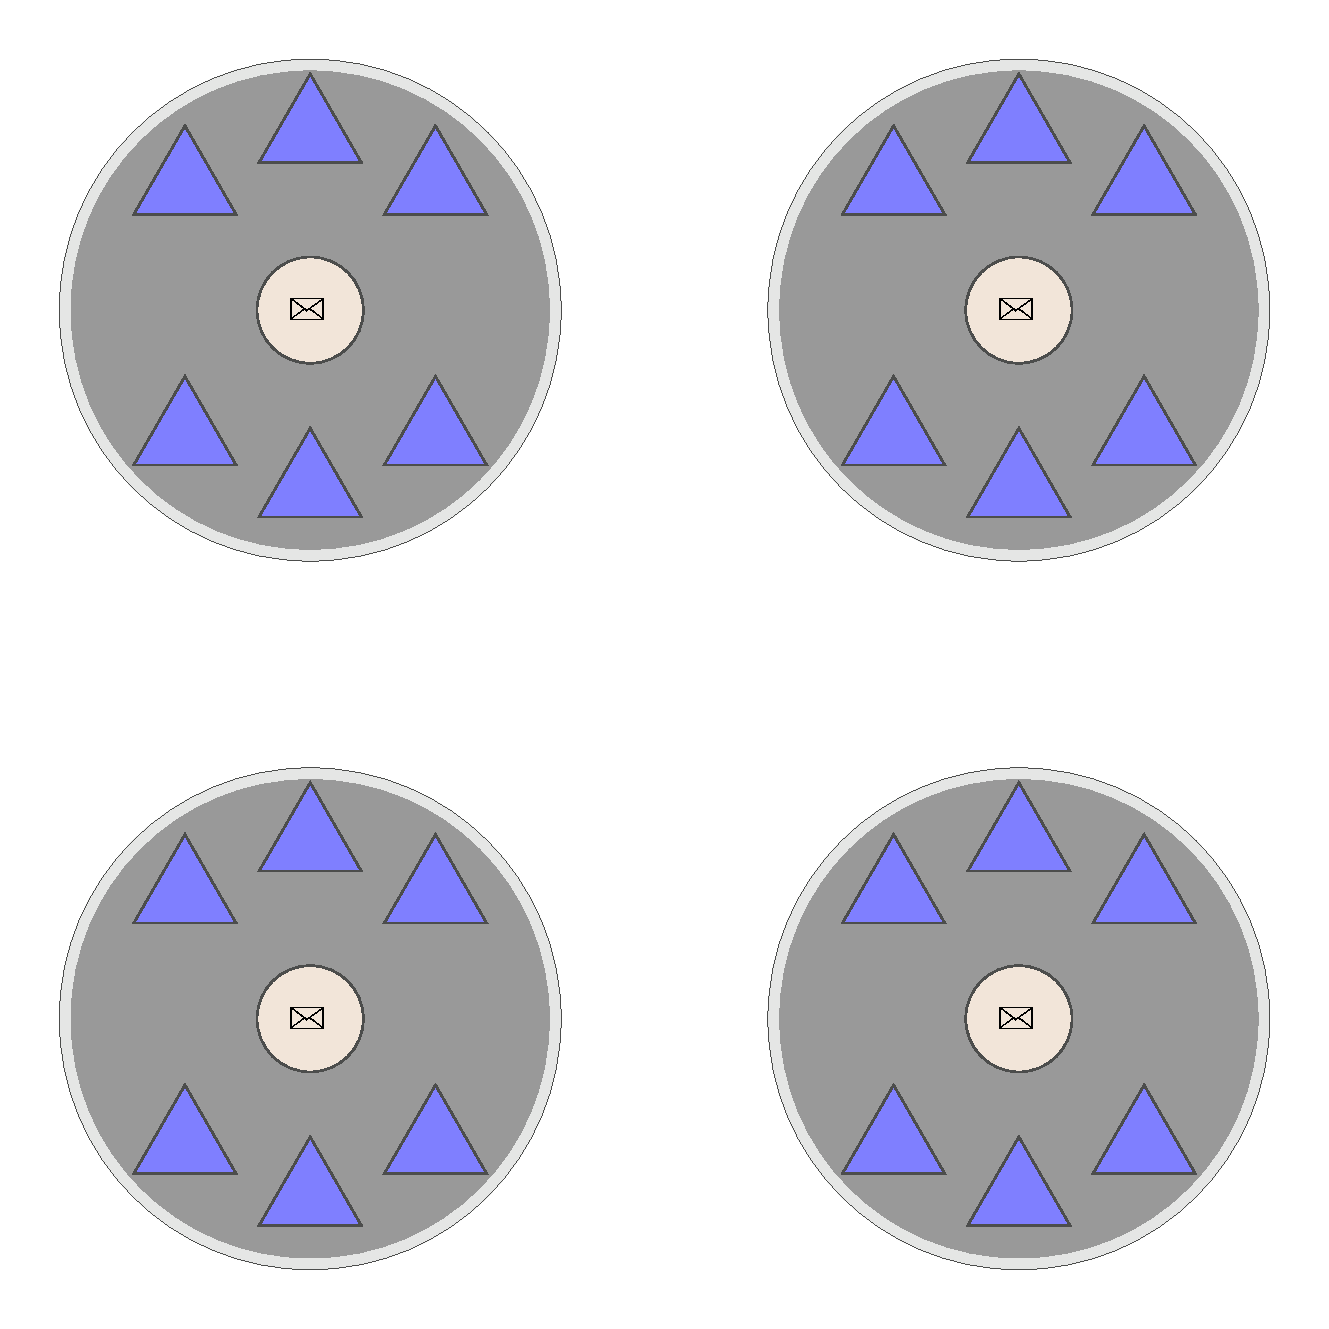
\includegraphics[width=3.5cm]{pictures/ae_01_1.pdf}}
	    \label{fig:exseqAS1}
	}
	\subfloat[][Step 2]{
		\fbox{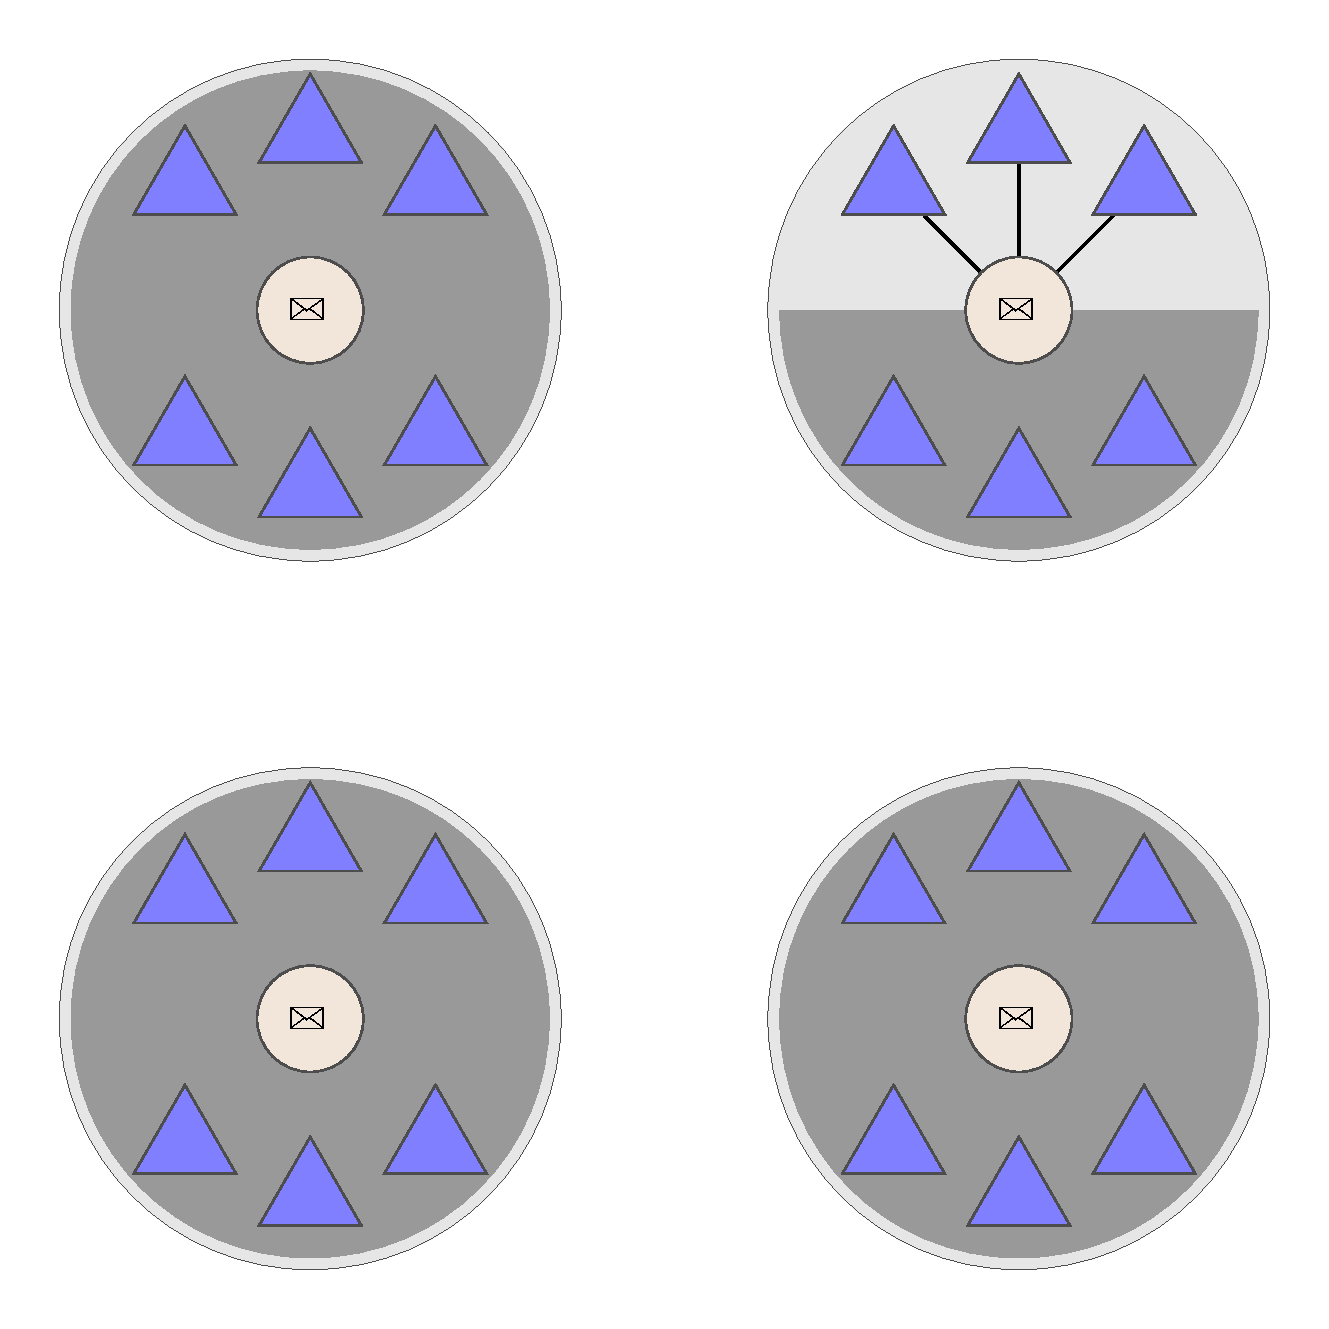
\includegraphics[width=3.5cm]{pictures/ae_01_2.pdf}}
	    \label{fig:exseqAS2}
	}
	\subfloat[][Step 3 (\lit true)]{ 
		\fbox{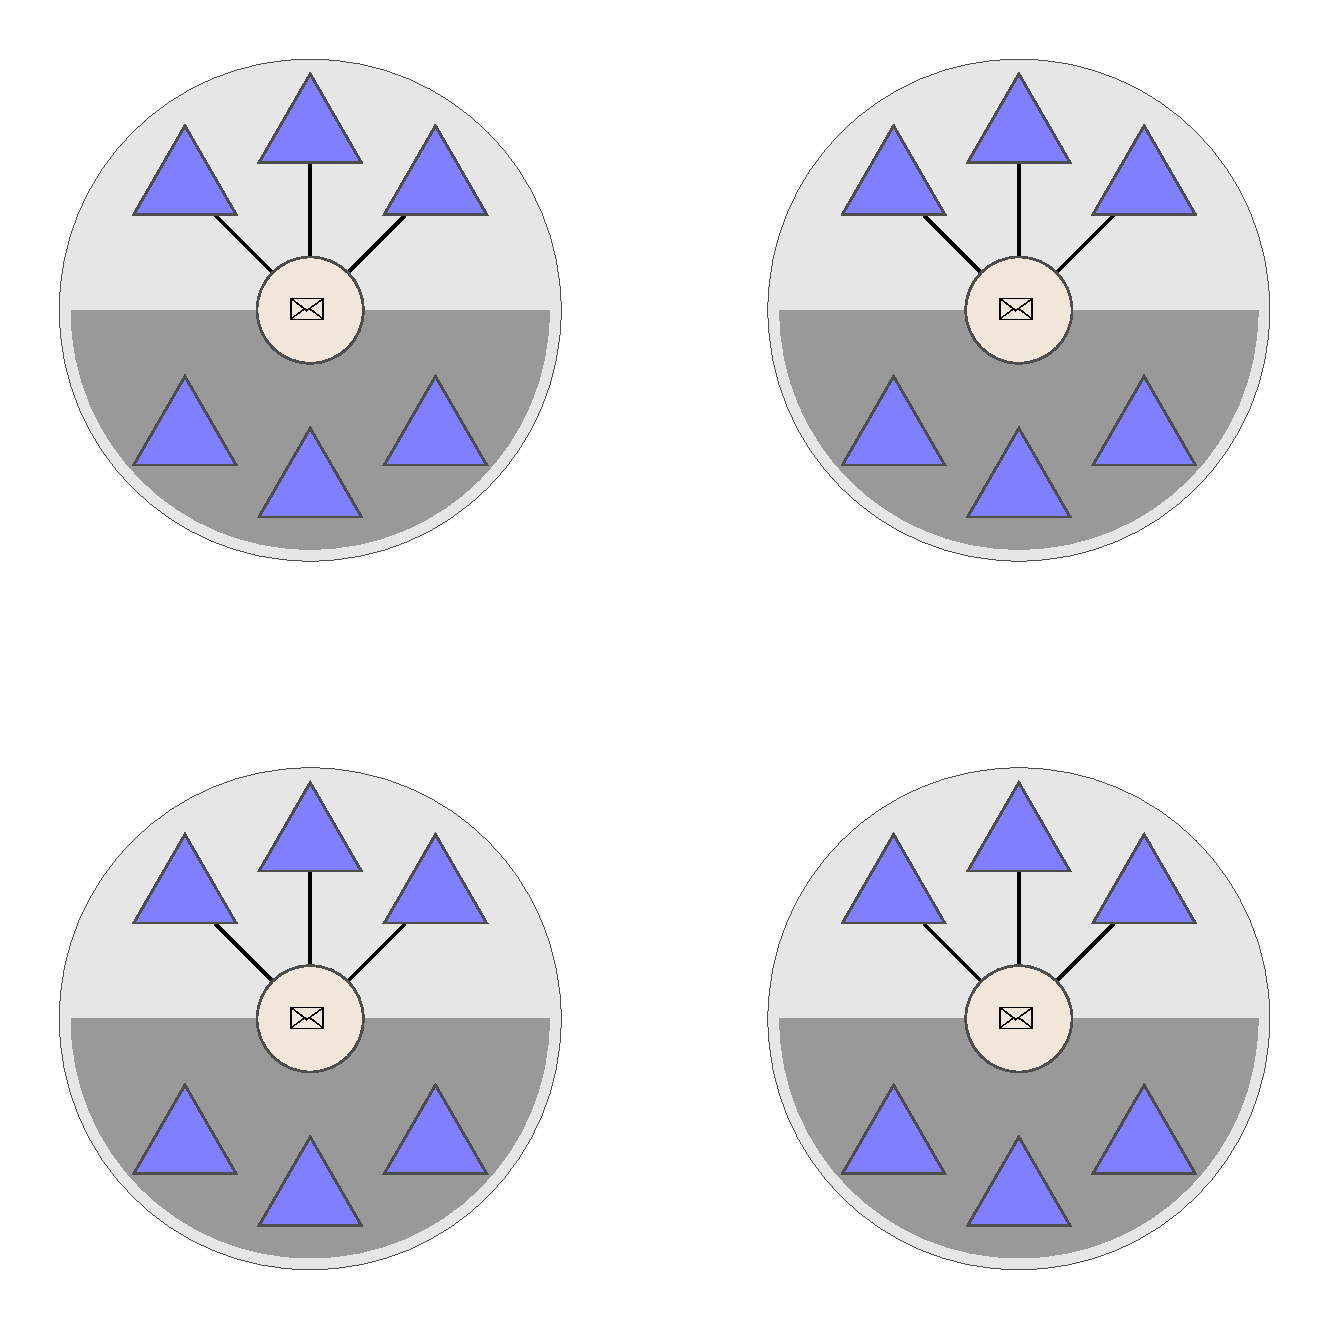
\includegraphics[width=3.5cm]{pictures/ae_01_3.pdf}}
	    \label{fig:exseqAS3}
	}
        \\
	\subfloat[][Step 4]{ 
		\fbox{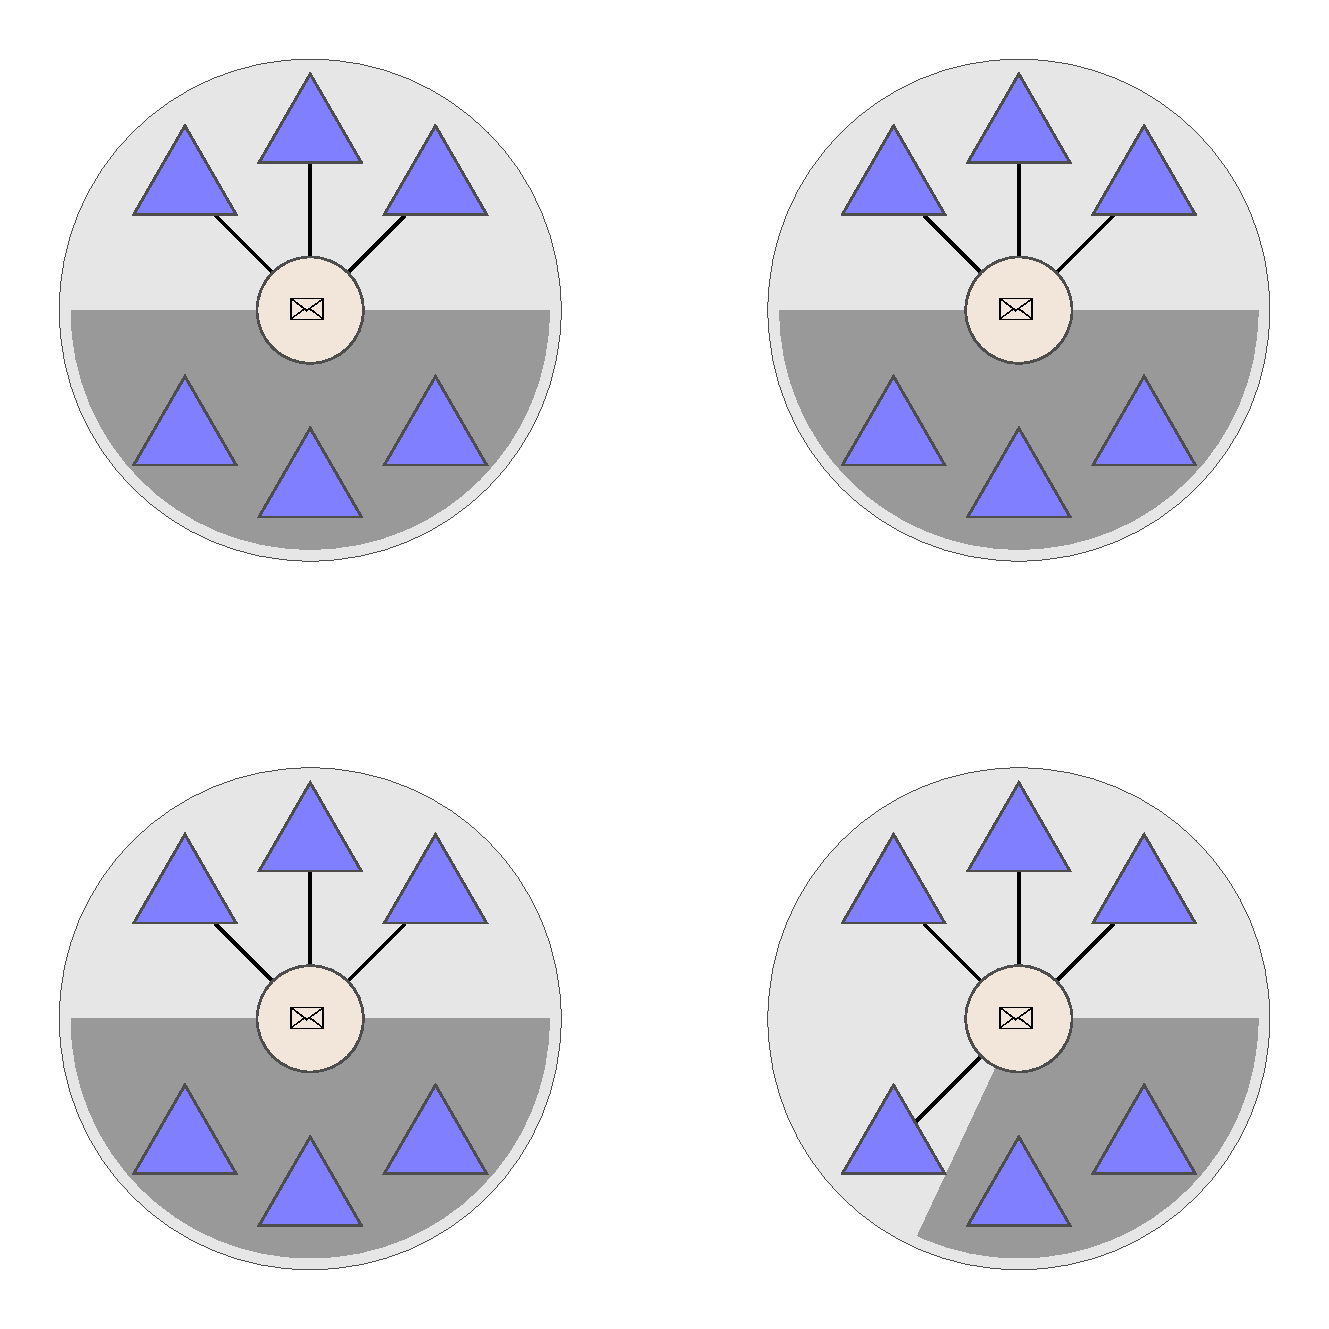
\includegraphics[width=3.5cm]{pictures/ae_01_4.pdf}}
	    \label{fig:exseqAS4}
	}
	\subfloat[][Step 5 (\glb true)]{
		\fbox{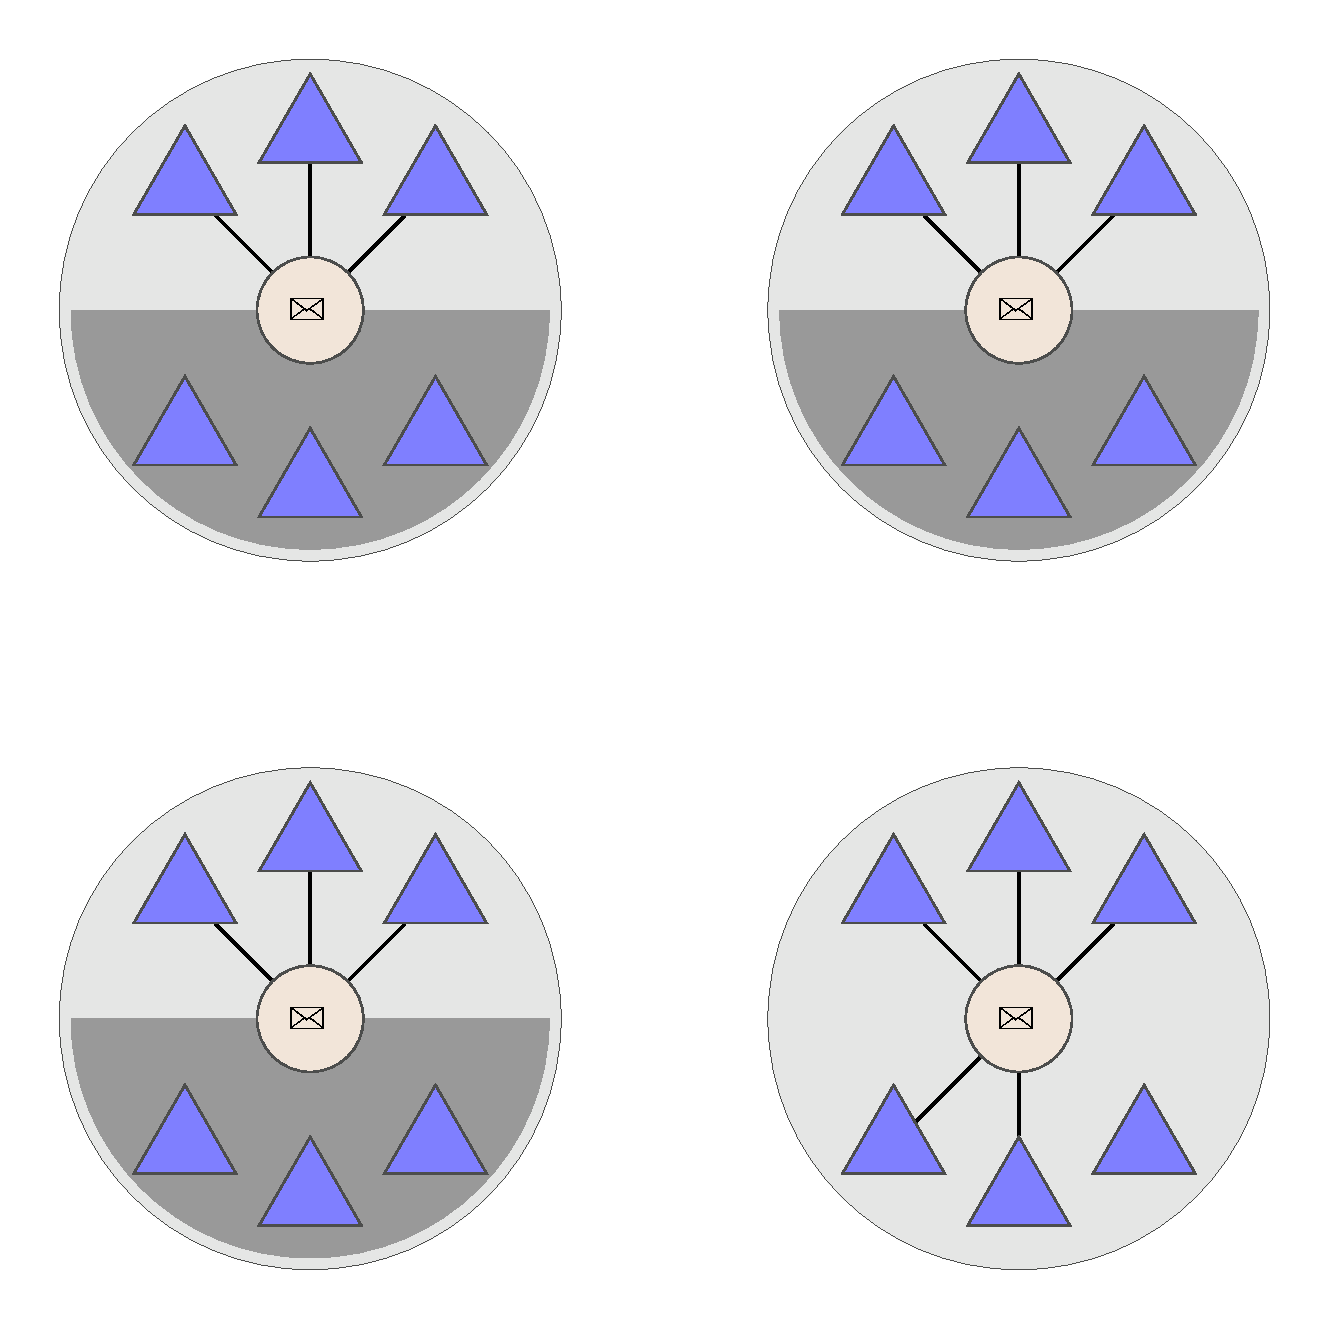
\includegraphics[width=3.5cm]{pictures/ae_01_5.pdf}}
	    \label{fig:exseqAS5}
	}
	\subfloat[][Step 6]{ 
		\fbox{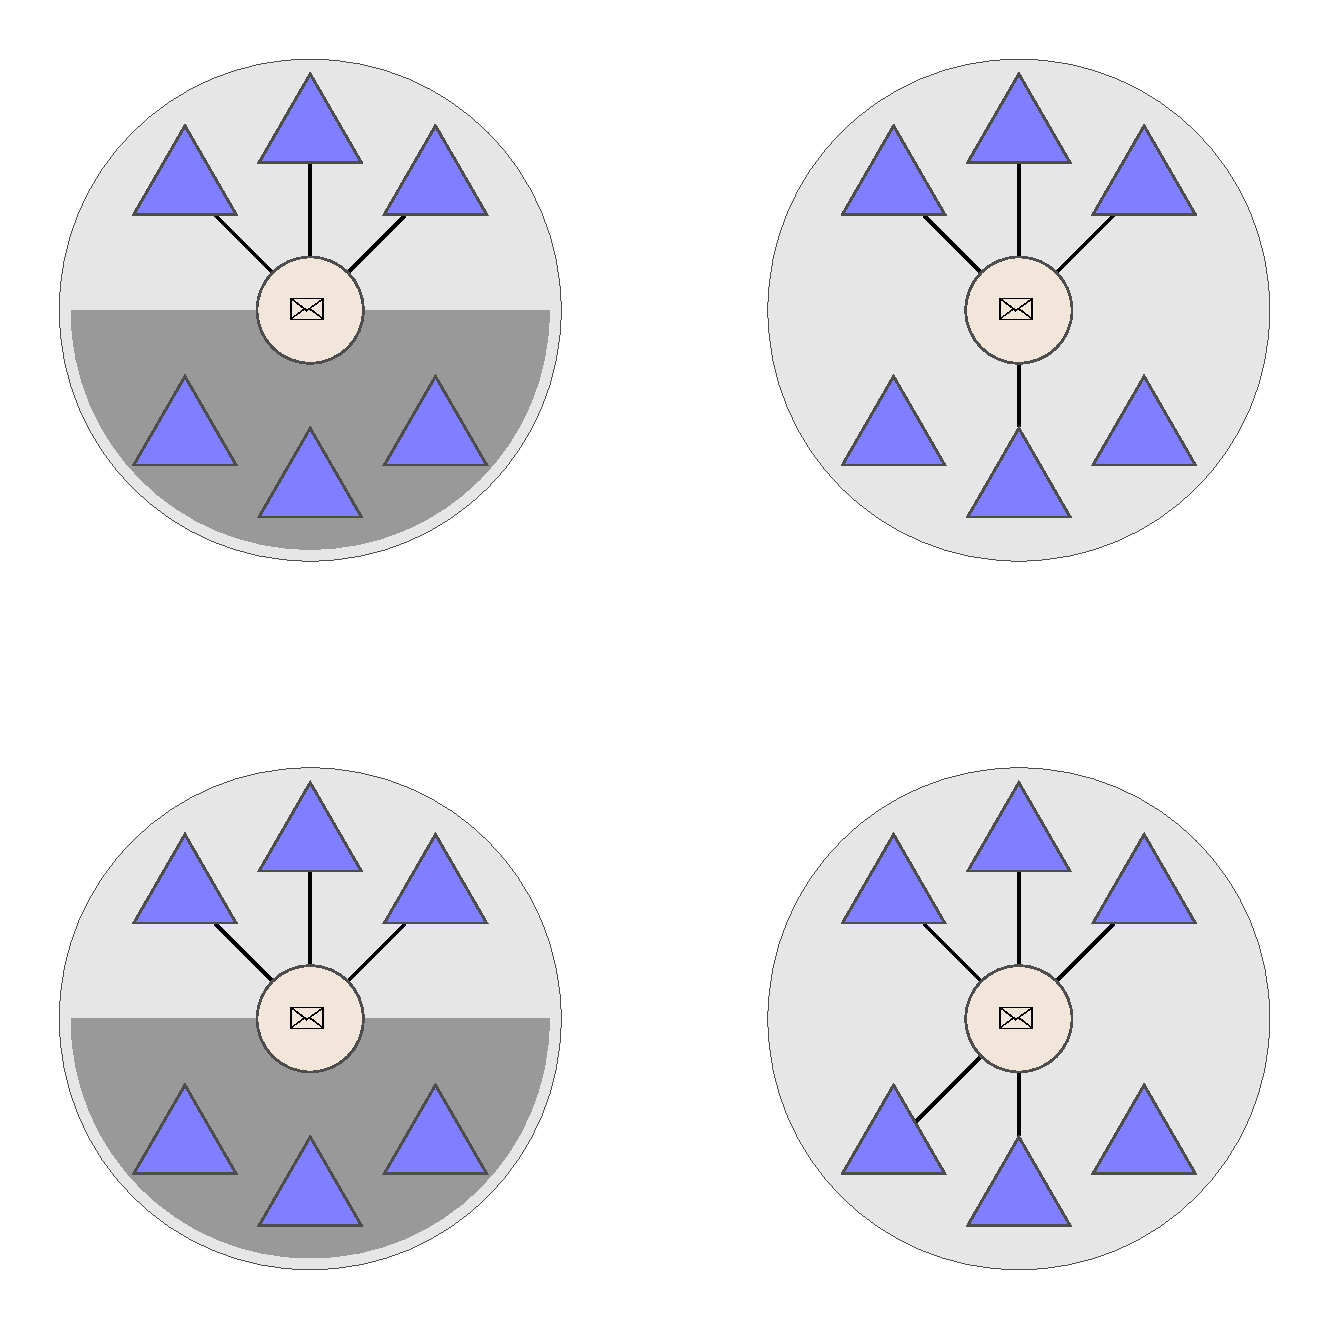
\includegraphics[width=3.5cm]{pictures/ae_01_6.pdf}}
	    \label{fig:exseqAS6}
	}
        \\
	\subfloat[][Step 7 (\loc false)]{ 
		\fbox{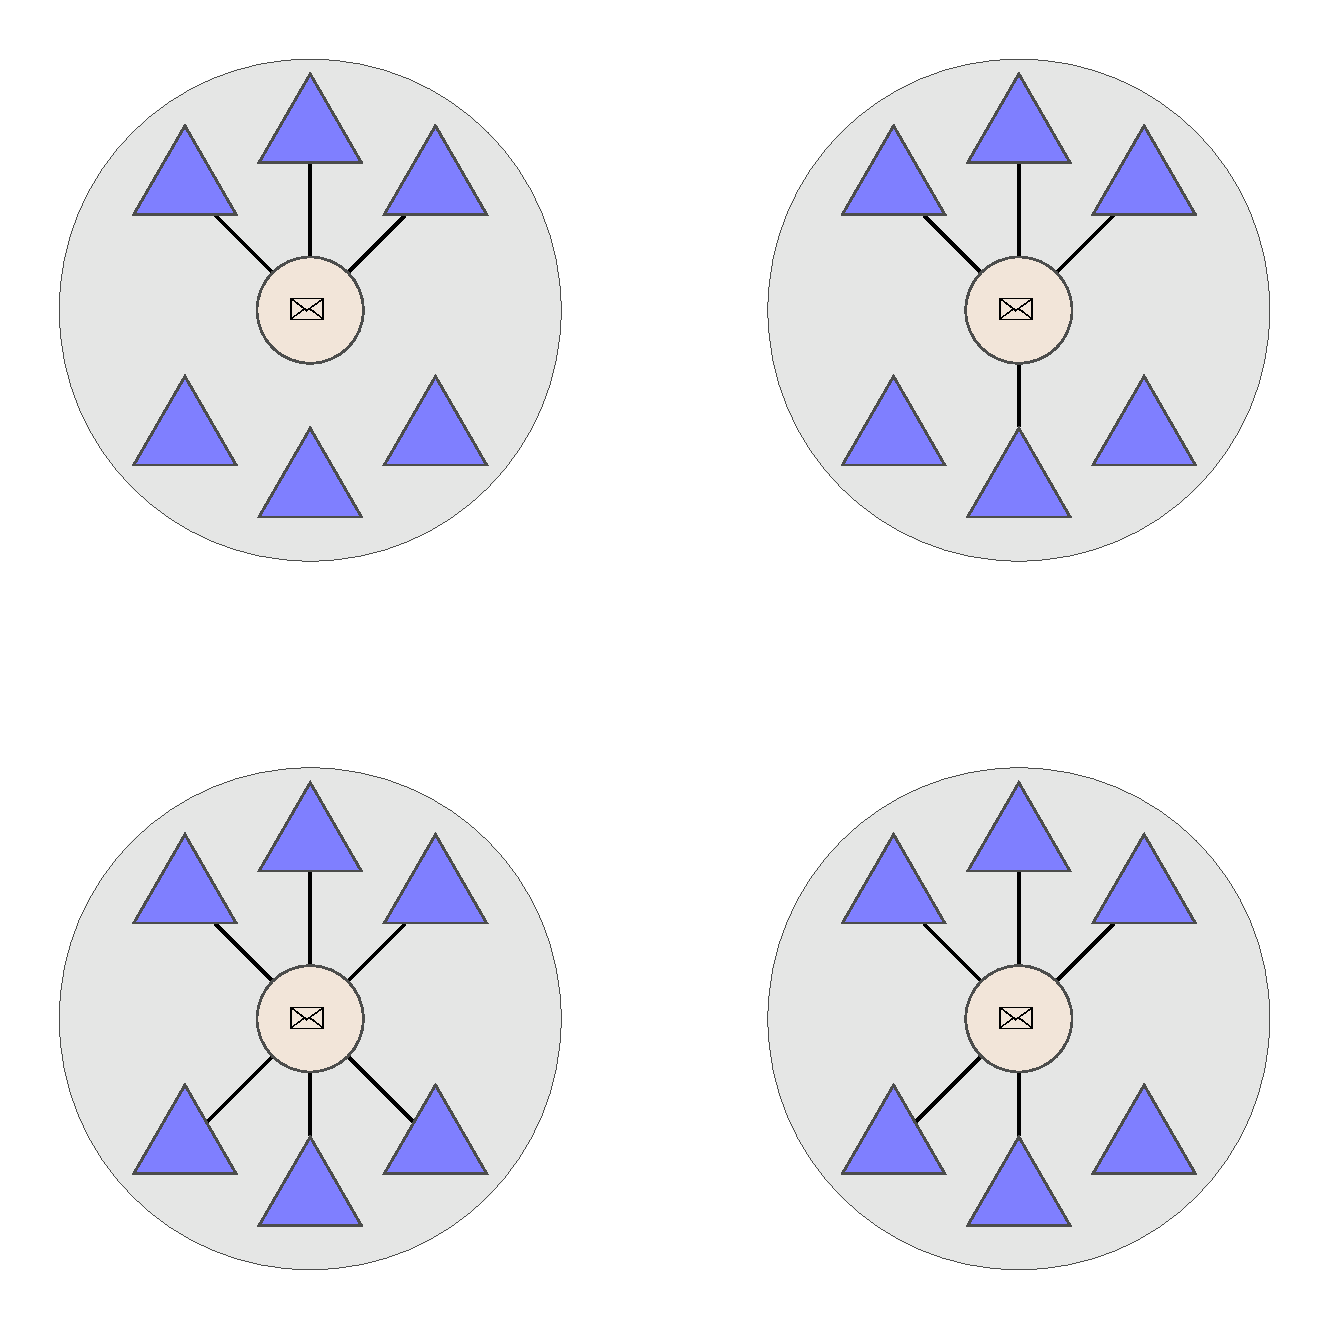
\includegraphics[width=3.5cm]{pictures/ae_01_7.pdf}}
	    \label{fig:exseqAS7}
	} 
                \hspace*{7.85cm} 
	\caption[]{Example picture sequence for \as-sentences.}
	\label{fig:exseqAS}
\end{figure}


Consider the German \as-sentence in (\ref{ex:as}), included in our study.
\begin{exe}
\ex \gll \mymark{Alle} diese Briefe sind mit \mymark{einigen} ihrer Dreiecke
  verbunden.\label{ex:as}\\
All these letters are with some their triangles connected.\\
\trans All of these letters are connected to some of their triangles.
\end{exe}
Figure~\ref{fig:exseqAS} shows the corresponding picture sequence. The
critical positions are on step 3, 5 and 7. Pictures that were
interspersed between these positions served as
spillover-pictures. These were used in order to counter potentially
delayed judgments and they additionally served as distractor
items. Prior to step 3 there is not enough information to judge any
candiate reading true or false. The situation at step 3 in
Figure~\ref{fig:exseqAS3} is true under a literal reading, while the
local and global readings cannot be evaluated yet. On step 5 in
Figure~\ref{fig:exseqAS5} the literal reading is still true, but now
also the global reading can be confirmed. Finally, decisions
concerning the local reading are possible as soon as all connections
have been uncovered at step 7 in Figure~\ref{fig:exseqAS7}. Note that
the situation at step 7 is \emph{in}compatible with a local
reading. This enables us to separate local readings, which would yield
\emph{false} judgements at this position, from literal and global
readings, which would yield \emph{true} judgements. In sum,
\emph{true} or \emph{false} answers on particular positions in the
incrementally revealed picture sequence can be mapped uniquely to
candidate readings. All other \emph{true} or \emph{false} answers were
counted as errors.

Due to the non-linear entailment order of readings described in
Section~\ref{sec:get-know-your}, \es-sentences require a slightly
different sequence of unfolding, which yields a different order in
which truth-value judgments can be made.
%
\begin{figure}[t]
	\centering
	\subfloat[][Step 1]{ 
		\fbox{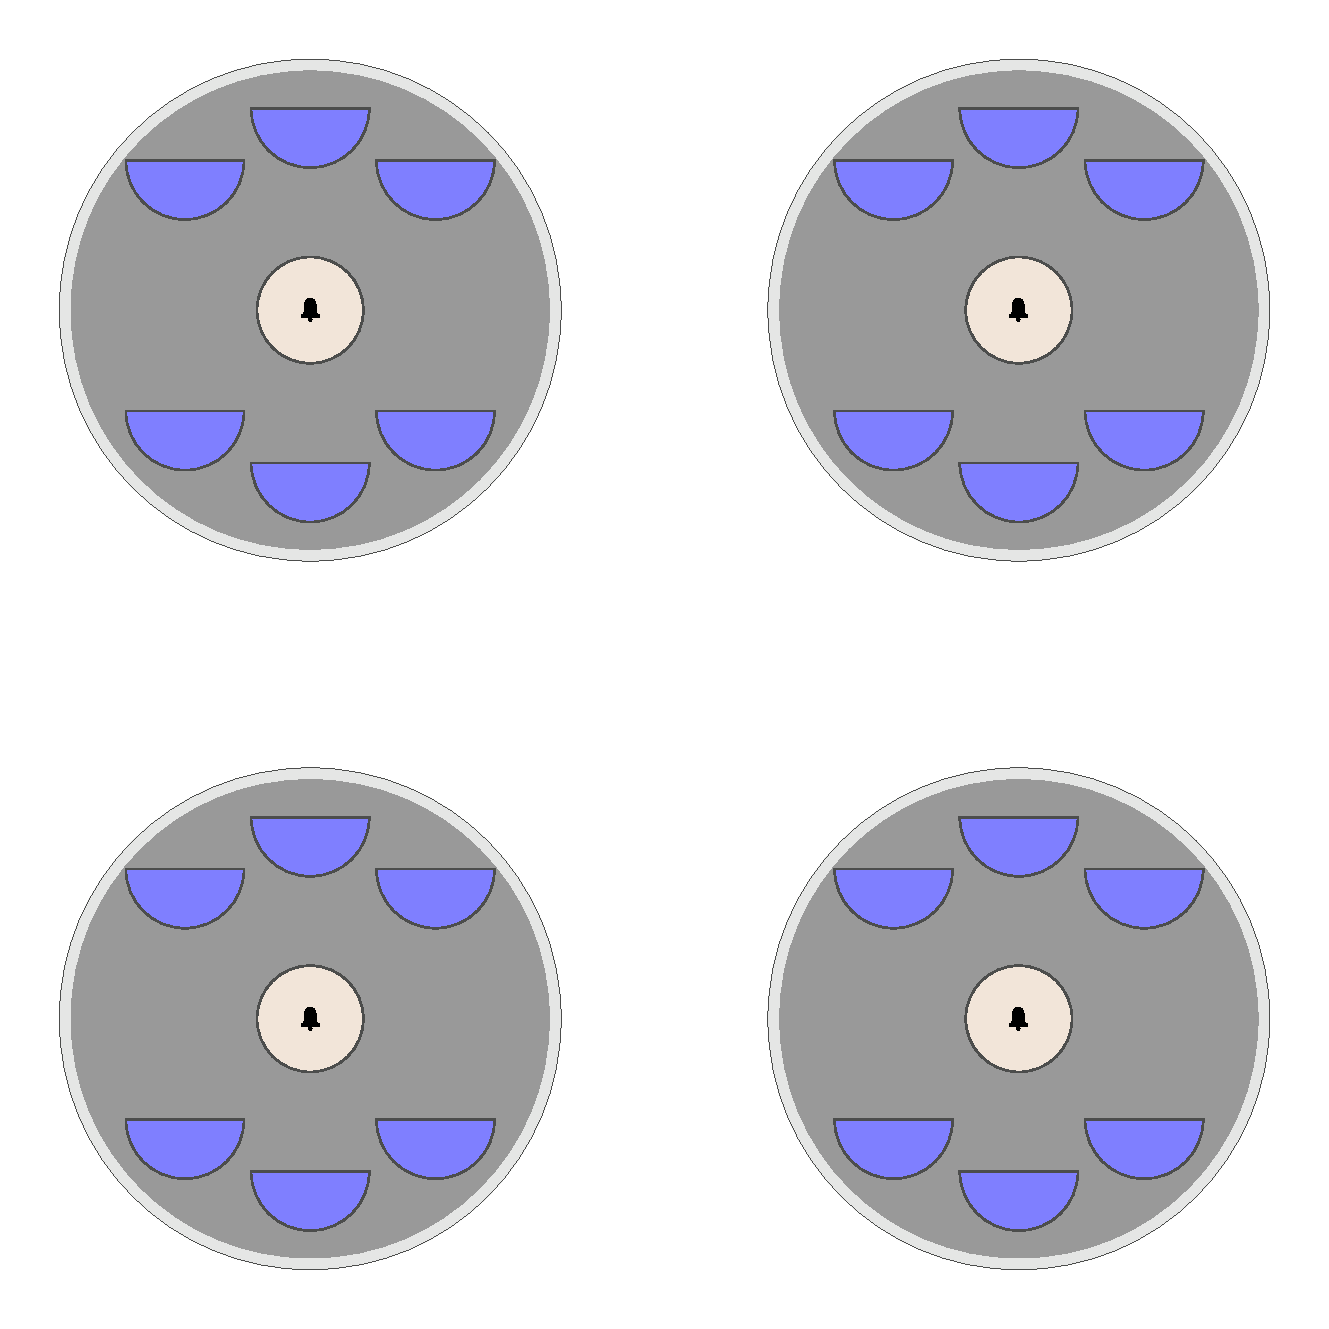
\includegraphics[width=3.5cm]{pictures/ge_01_1.pdf}}
	    \label{fig:exseqES1}
	}
	\subfloat[][Step 2 (\glb false)]{
		\fbox{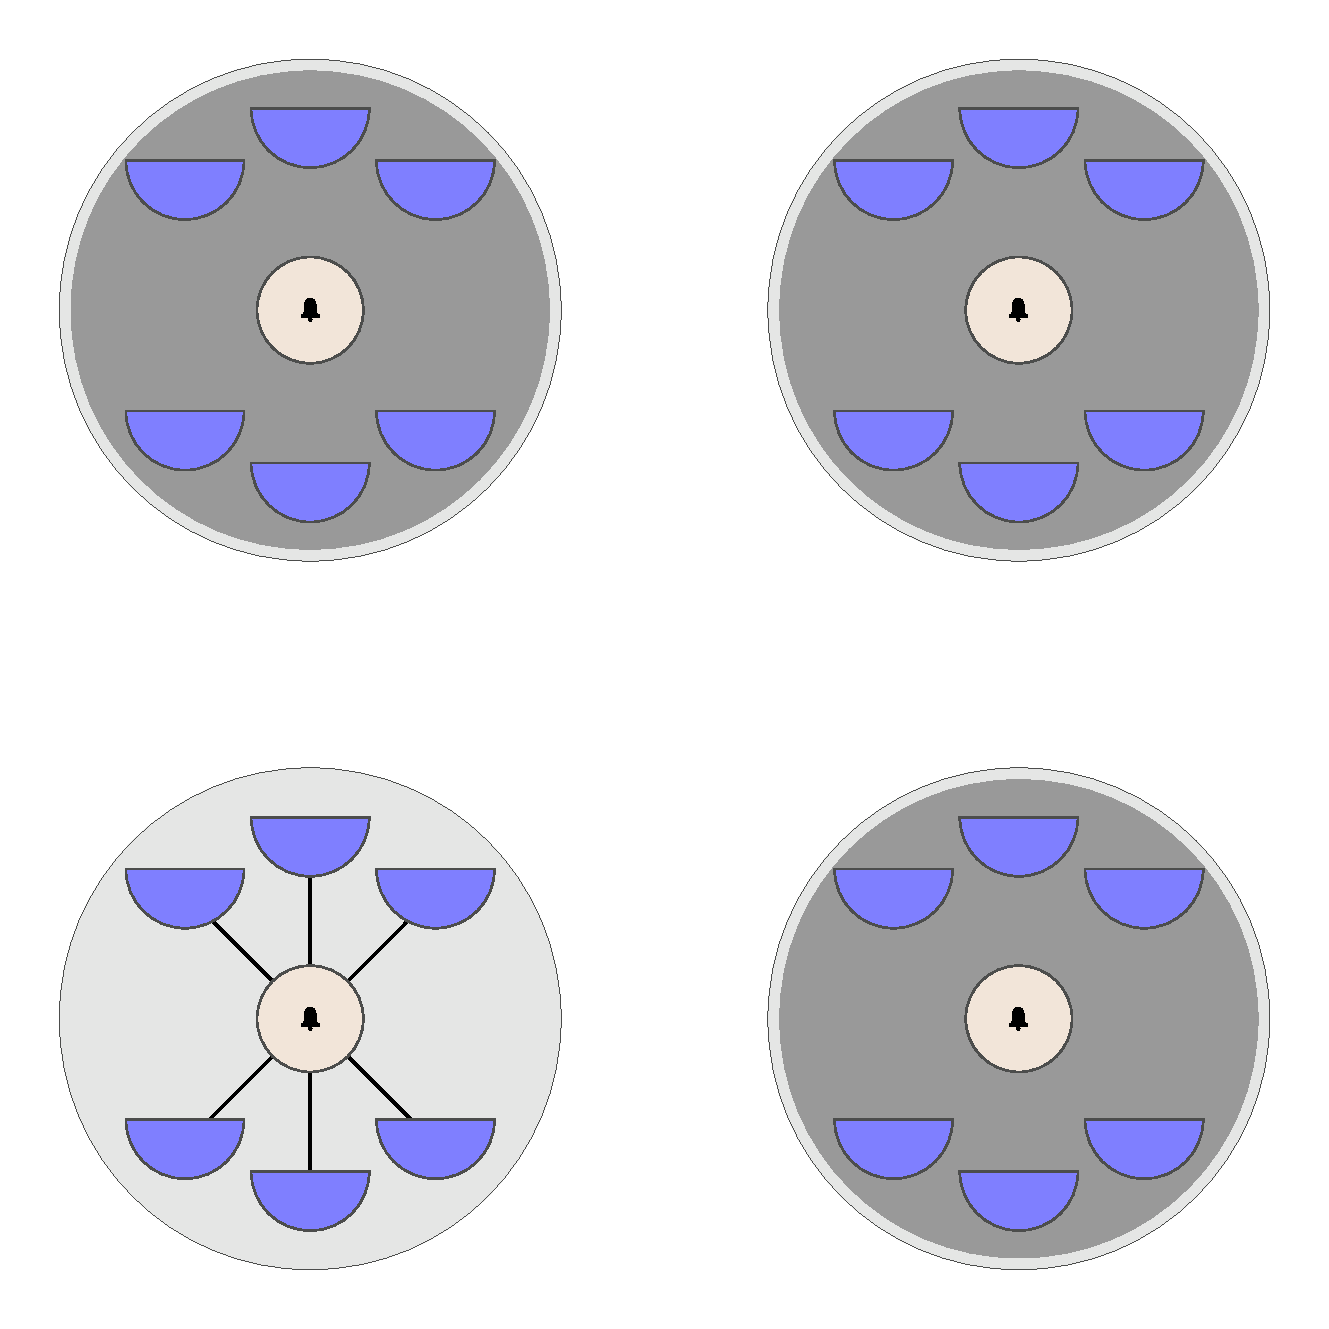
\includegraphics[width=3.5cm]{pictures/ge_01_2.pdf}}
	    \label{fig:exseqES2}
	}
	\subfloat[][Step 3 (\lit false)]{ 
		\fbox{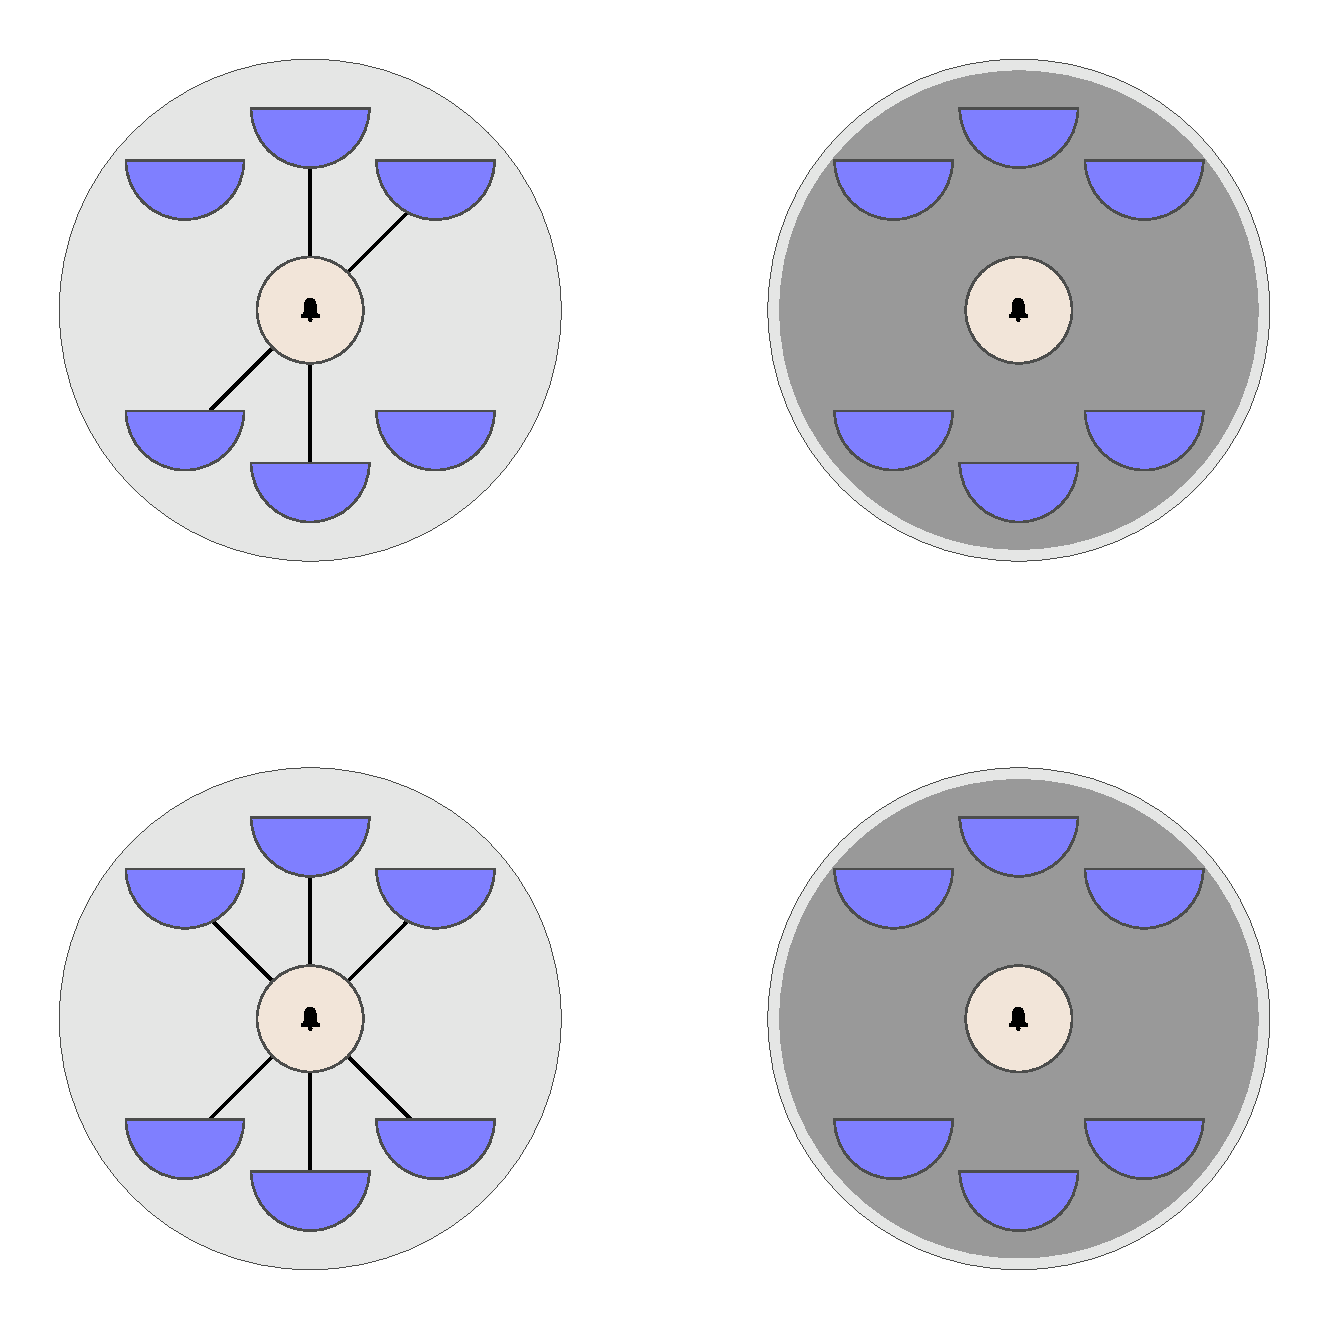
\includegraphics[width=3.5cm]{pictures/ge_01_3.pdf}}
	    \label{fig:exseqES3}
	}
        \\
	\subfloat[][Step 4]{ 
		\fbox{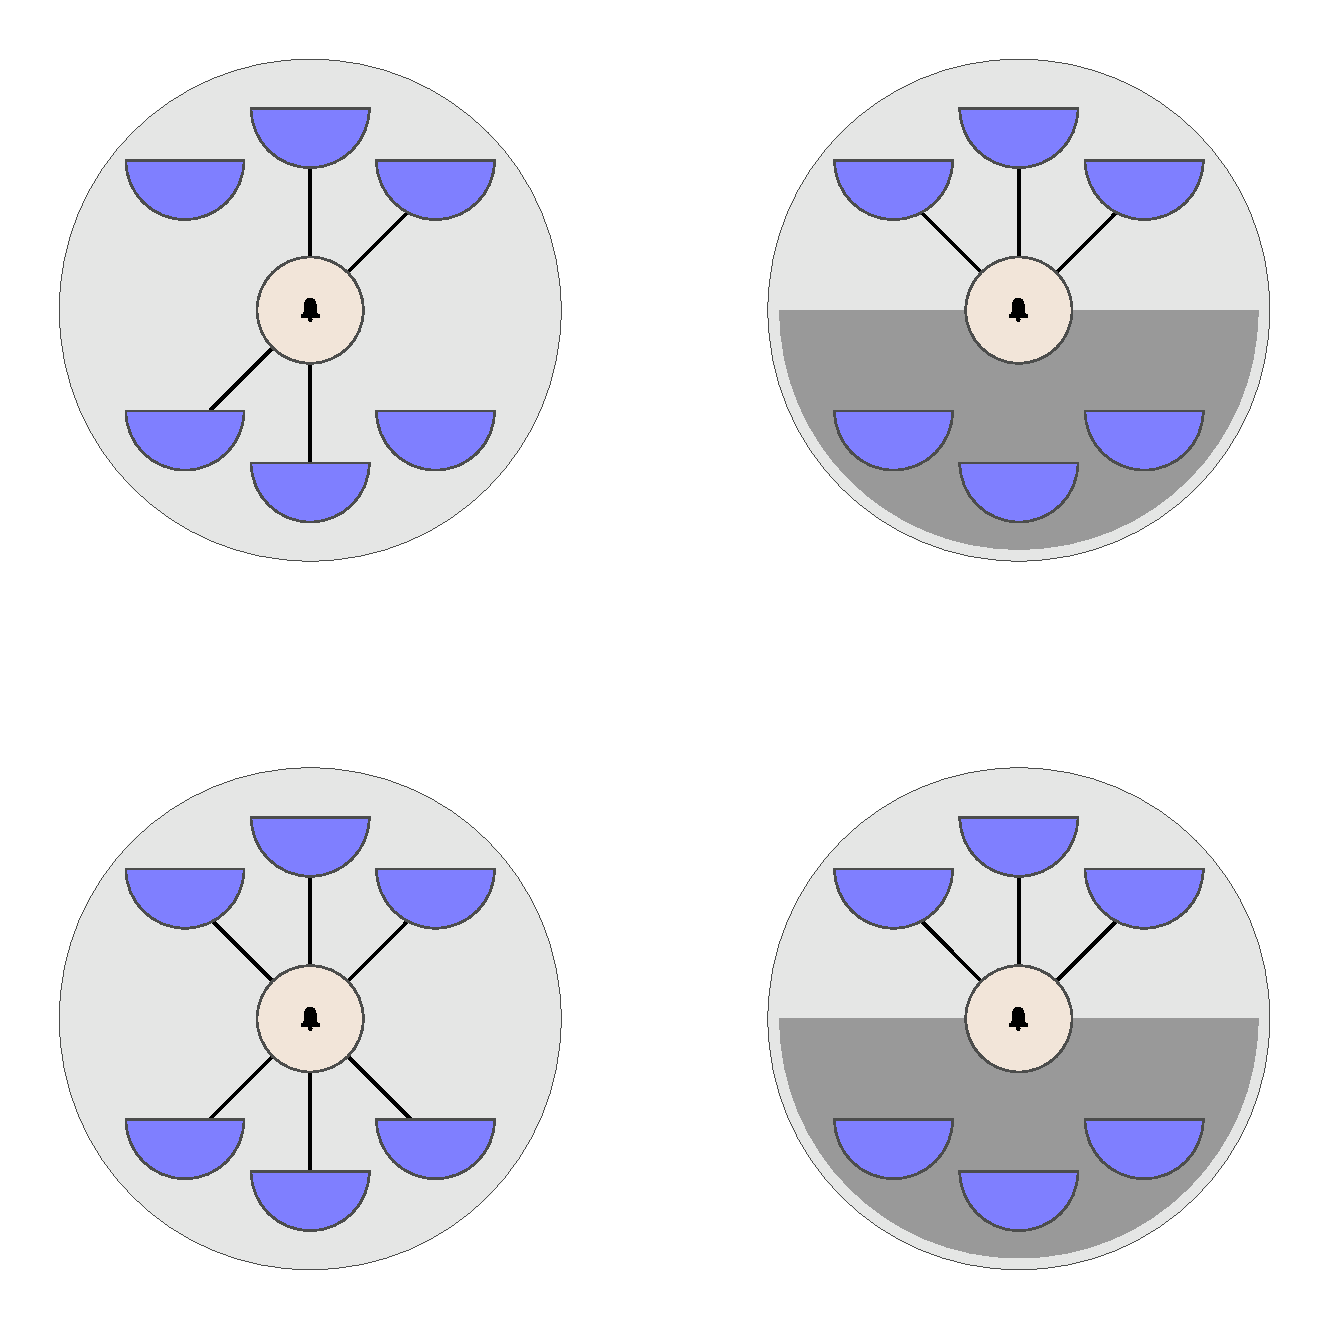
\includegraphics[width=3.5cm]{pictures/ge_01_4.pdf}}
	    \label{fig:exseqES4}
	}
	\subfloat[][Step 5 (\loc true)]{
		\fbox{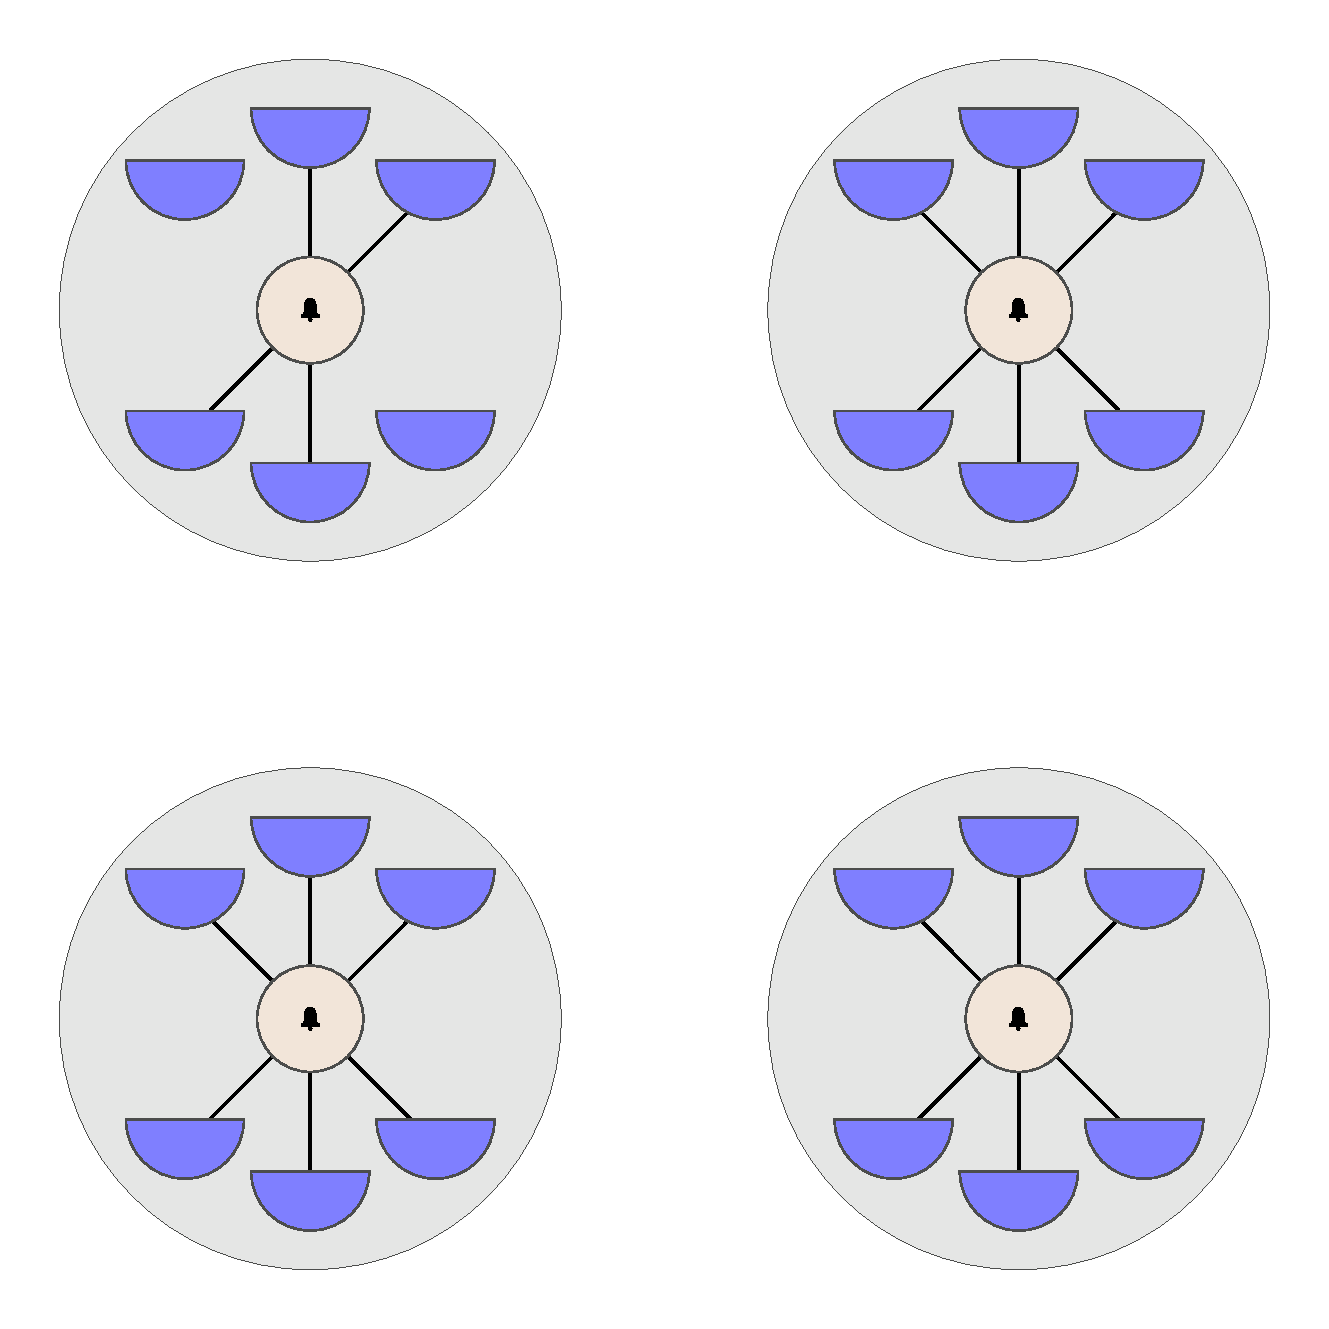
\includegraphics[width=3.5cm]{pictures/ge_01_5.pdf}}
	    \label{fig:exseqES5}
	}
                \hspace*{3.9cm} 
	\caption[]{Example sequence for \es-sentences.}
	\label{fig:exseqES}
\end{figure}
%
For a sentence like (\ref{ex:es}), we obtain an unambiguous mapping
between truth judgements and readings with the sequence in
\ref{fig:exseqES}.
\begin{exe}
\ex \label{ex:es} \gll \mymark{Genau} eine der Glocken ist mit
  \mymark{einigen} ihrer Halbkreise verbunden.\\ 
  Exactly one of-the bells is with some its semicircles connected.\\
  \trans Exactly one bell is connected to some of its semicircless.
\end{exe}
The critical positions are steps 2, 3 and 5. At step 2 in
Figure~\ref{fig:exseqES2}, a global reading would yield a \emph{false}
judgement. The literal reading can be evaluated at step 3 in
Figure~\ref{fig:exseqES3}, where it would trigger a \emph{false}
judgement. Finally, confirming \ref{fig:exseqES5} by a \emph{true}
response indicates a local reading. Note that global and literal
readings again differ from local readings with respect to their truth
values.


\paragraph{Positional controls.} To make sure that subjects understood
the task, i.e., gave truth-value judgements at the first possible
position in a sequence, we included a set of control conditions. These
also controlled for response biases. For each of the three readings in
the \as- and \es-conditions, we constructed an unambiguous control
sentence as in (\ref{bsp:controls-as}) and (\ref{bsp:controls-es}),
requiring the same judgement at the identical position in the same
sequence used for the respective targets. For instance, example
(\ref{bsp:controls-as-1}) requires a \emph{true}-response analogous to
the \as-sentence in (\ref{ex:as}) under its literal reading at step 3
in Figure~\ref{fig:exseqAS3}, (\ref{bsp:controls-as-2}) corresponds to
the \as-sentence under its global reading and
(\ref{bsp:controls-as-3}) corresponds to its local reading. With
regard to the \es-sentences, controls like (\ref{bsp:controls-es-1})
correspond to the global reading, (\ref{bsp:controls-es-2}) to the
literal and (\ref{bsp:controls-es-3}) to the local reading. If,
independently of sentence meaning, there was any bias to respond in a
certain way at any point in the sequences, such as to preferably
unravel the whole picture, this should affect control sentences to the
same degree as it affects target conditions.

\begin{exe}
  \ex \label{bsp:controls-as}
    \begin{xlist}
\ex \label{bsp:controls-as-1} \gll Alle Briefe sind mit mindestens drei ihrer Dreiecke verbunden.\\
  All letters are with at-least three their triangles connected.\\
  \trans All letters are connected to at least three of their triangles.
\ex \label{bsp:controls-as-2} \gll Mindestens ein Brief ist mit genau f\"unf seiner Dreiecke verbunden.\\
  At-least one letter is with exactly five his triangles connected.\\
  \trans At least one letter is connected with exactly five of its triangles.
\ex \label{bsp:controls-as-3} \gll Jeder Brief ist mit mindestens vier seiner Dreiecke verbunden.\\
  Every letter is with at-least four his triangles connected.\\
  \trans Every letter is connected to at least four of its triangles.
\end{xlist}
\end{exe}

\begin{exe}
\ex \label{bsp:controls-es}
  \begin{xlist}
\ex \label{bsp:controls-es-1} \gll Alle Glocken sind mit weniger als
  vier ihrer Halbkreise verbunden. \\ 
All bells are with fewer than four their semicircles connected.\\
\trans All bells are connected with fewer than four of their semicircles.  
\ex \label{bsp:controls-es-2} \gll Alle Glocken sind mit allen ihren Halbkreisen verbunden.\\
All bells are with all their semicircles connected.\\
\trans All bells are connected to all of their semicircles. 
\ex \label{bsp:controls-es-3} \gll Mindestens drei Glocken sind mit
  allen ihren Halbkreisen verbunden.\\ 
  At-least three bells are with all  their semicircles connected.\\
  \trans At least three bells are connectd with all of their semicircles.
\end{xlist}
\end{exe}

\paragraph{Preference-related controls.} In order to test whether the
order of critical positions for different readings within a sequence
had an influence on responses, we included a second type of control
conditions.  These controls also tested whether the incremental
verification task could possibly detect at least ordinal preference
relations among multiple candidate readings. Note that for our target
sentences, the logical entailment relations between readings always
require local readings to be evaluated at the end of a sequence. It
could be that subjects never reach this point, because they give
truth-value judgements earlier, thereby ending the trial. In that case
it would be unclear whether these decisions had been affected by a
general unavailability of local readings or by the fact that one of
the earlier presented readings is the preferred one. By including
globally ambiguous structures with a known preference over available
readings, we thus tested whether participants in our task occasionally
choose dispreferred readings, even if these were available only at a
critical position following the preferred readings. Finally, these
conditions also controlled whether prosodic information can, in
principle, shift answer patterns in the present task.

We therefore included sentences with \emph{attachment ambiguities} as
in (\ref{bsp:target-related}), which have been shown to exhibit
interpretive preferences and can be disambiguated by prosodic
information.\footnote{It is possible that attachment ambiguities are
  different from the ``pragmatic ambiguity'' in \as- and
  \es-sentences, so that information about the former is not ideally
  informative about the latter. We will address this worry in
  Section~\ref{sec:critical-reflection}, where we argue that this does
  not affect the main conclusion that we would like to draw from our
  data eventually.}

\begin{exe}
\ex \gll Der Brief ist mit Kreisen und Vierecken mit Sonnen
  verbunden. \label{bsp:target-related}\\
The letter is with circles and squares with suns connected.\\
The letter is connected with circles and squares with suns.
\begin{xlist}
  \ex \label{bsp:target-related-LC} The letter is connected with squares containing suns, and it is
    also connected with circles. \hfill{(\lc)}
  \ex \label{bsp:target-related-EC} The letter is connected with circles and squares, both of which
    are containing suns.  \hfill{(\ec)} 
\end{xlist}
\end{exe}
In attachment ambiguities involving post-nominal modification, an
adjunct like a relative clause or a prepositional phrase (\acro{pp})
can be attached to one of two preceding hosts.  For instance, in
(\ref{bsp:target-related}), the \acro{pp} \emph{with suns} can be
attached to the preceding noun \emph{squares}, resulting in the
so-called \emph{late-closure} (\lc) reading
((\ref{bsp:target-related-LC}). Alternatively, the \acro{pp} can be
attached to the whole conjunctive \acro{np} \emph{circles and
  squares}, corresponding to the \emph{early-closure} (\ec) reading
(\ref{bsp:target-related-EC}).  \lc-readings have been generally
observed to be preferred over \ec-readings (e.g., \cite{Fodor98} for
an overview of different languages, but see also
\cite{CliftonCarlsonFrazier2002} for counterevidence). Crucially, an
\lc-preference for \acro{pp}-attachment structures has also been
attested for German \citep[][]{KoniecznyHemforth2000}.

For each sentence, two sequences were designed: one in which the
preferred \lc-reading could be judged first (Figure~\ref{fig:exlc}),
%
\begin{figure}[]
	\centering
	\subfloat[][Step 2]{ 
		\fbox{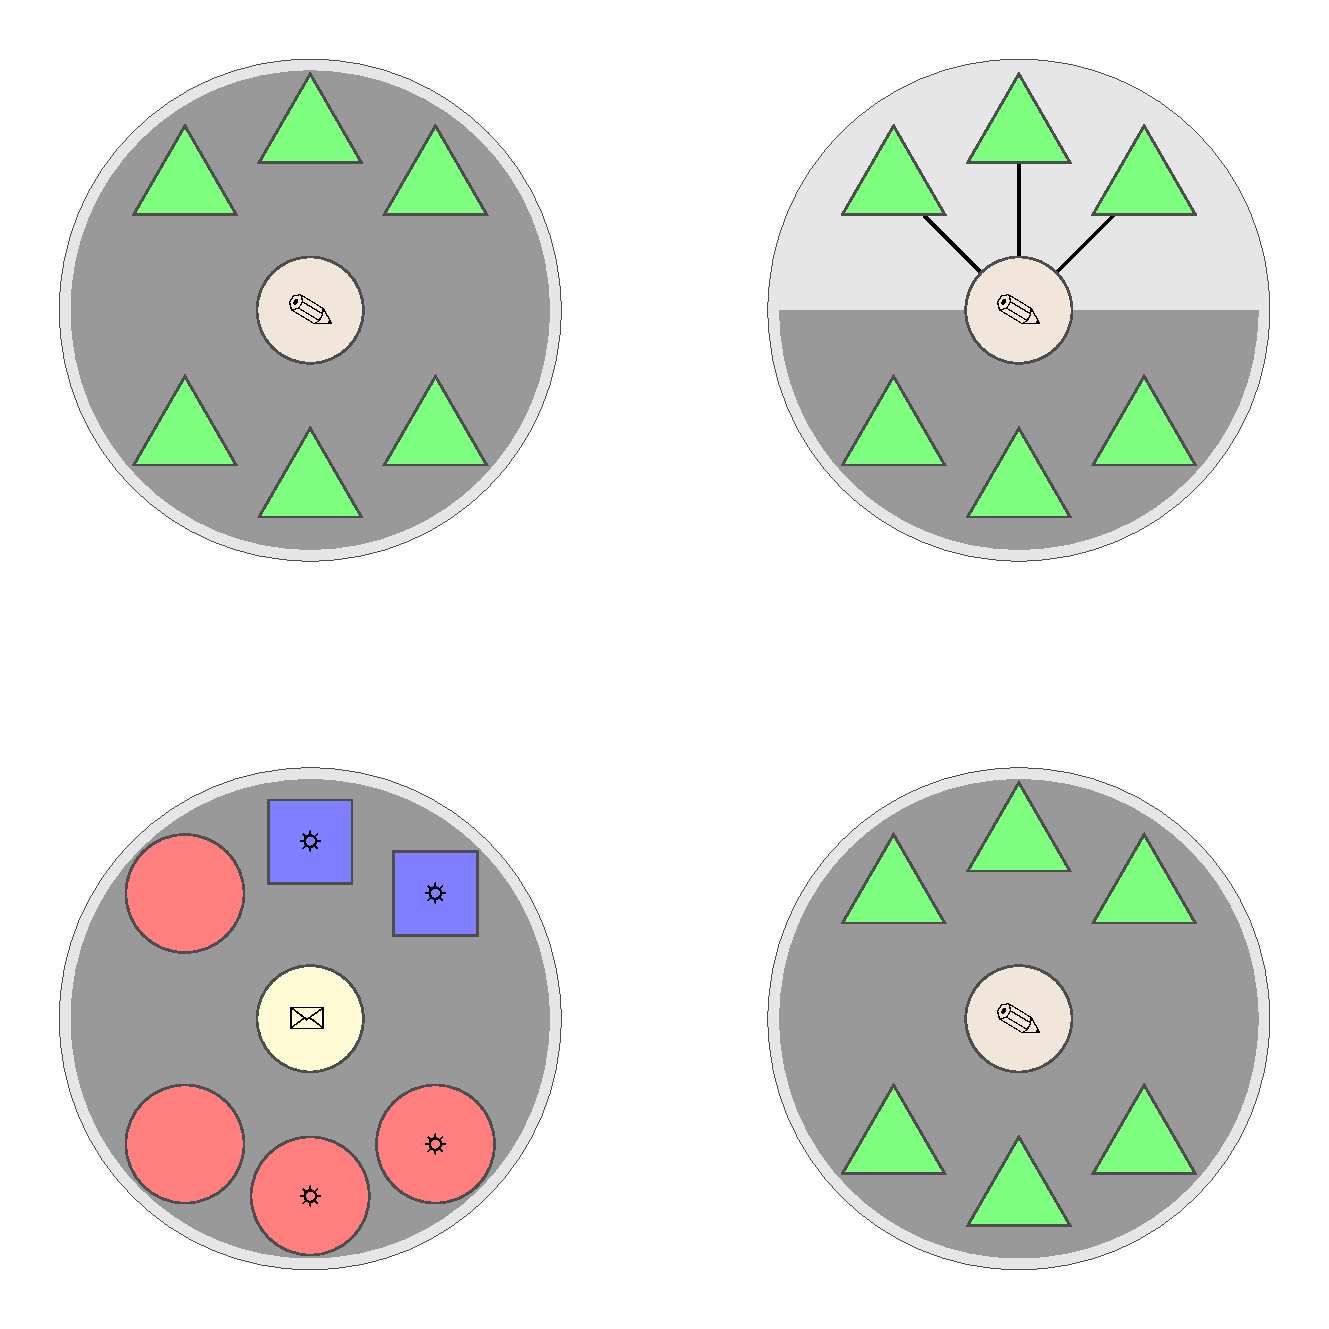
\includegraphics[width=5cm]{pictures/lc_01_2.pdf}}
	    \label{fig:exlc2}
	}
	\subfloat[][Step 3 (\lc true)]{
		\fbox{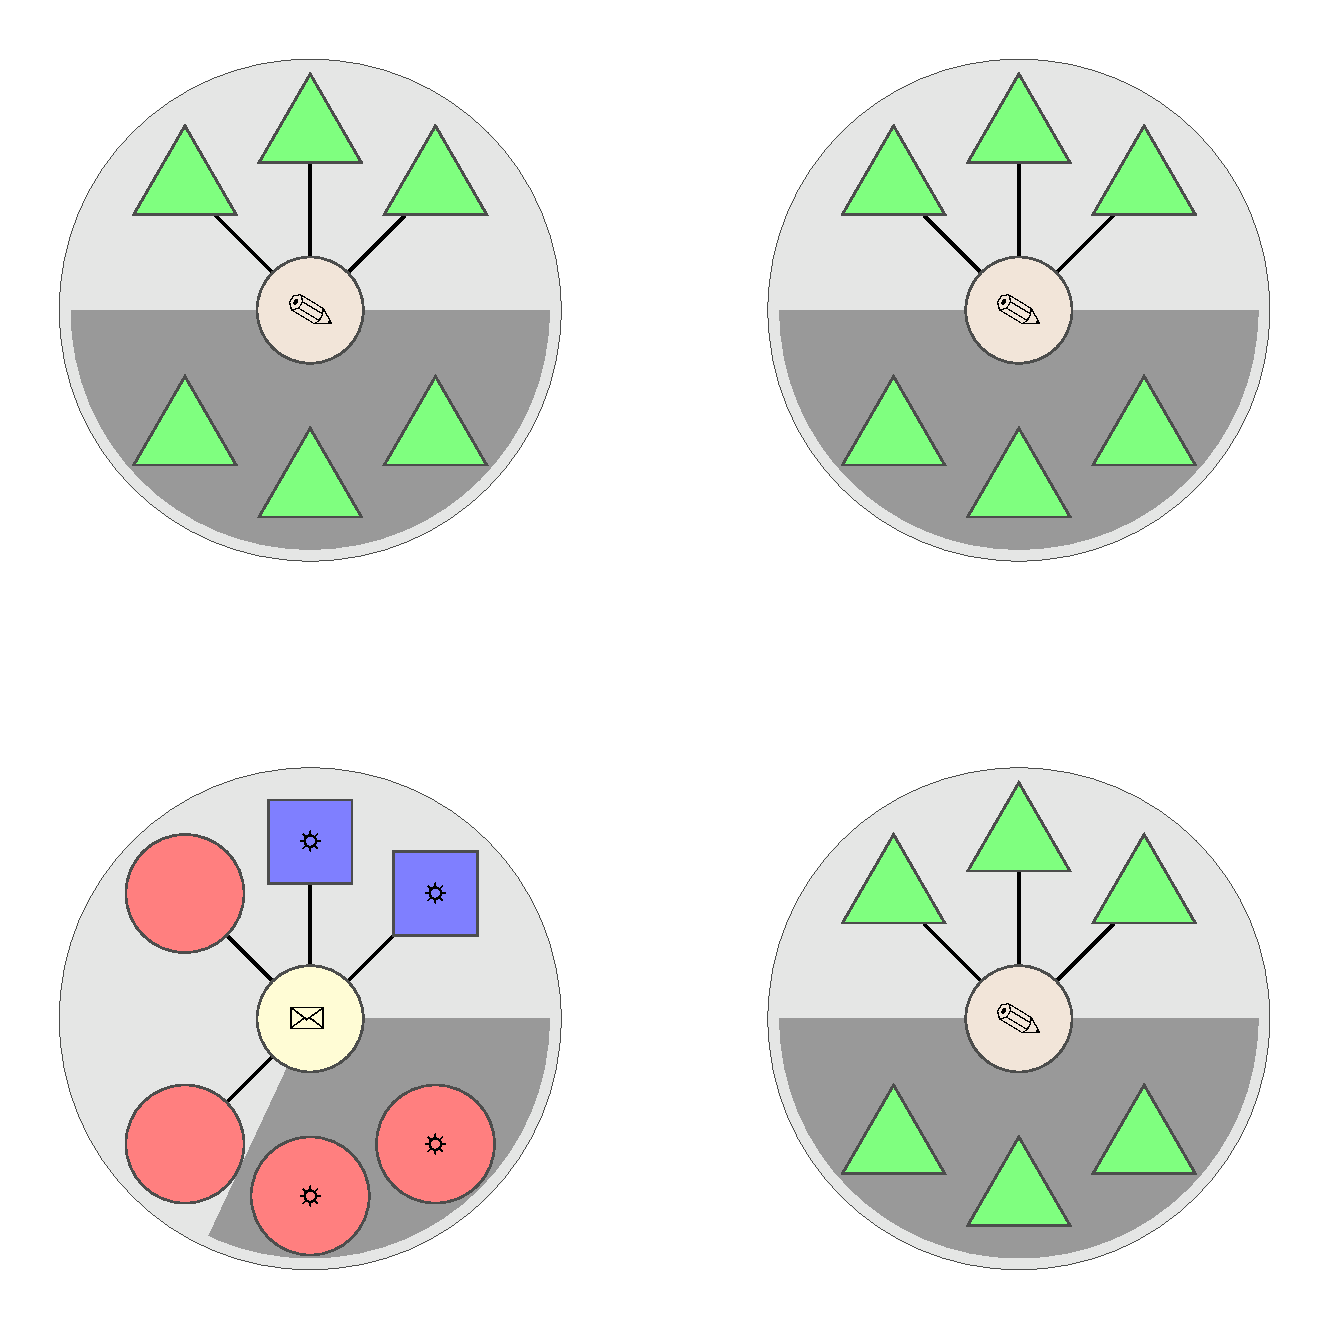
\includegraphics[width=5cm]{pictures/lc_01_3.pdf}}
	    \label{fig:exlc3}
	}
        \\
	\subfloat[][Step 4]{
		\fbox{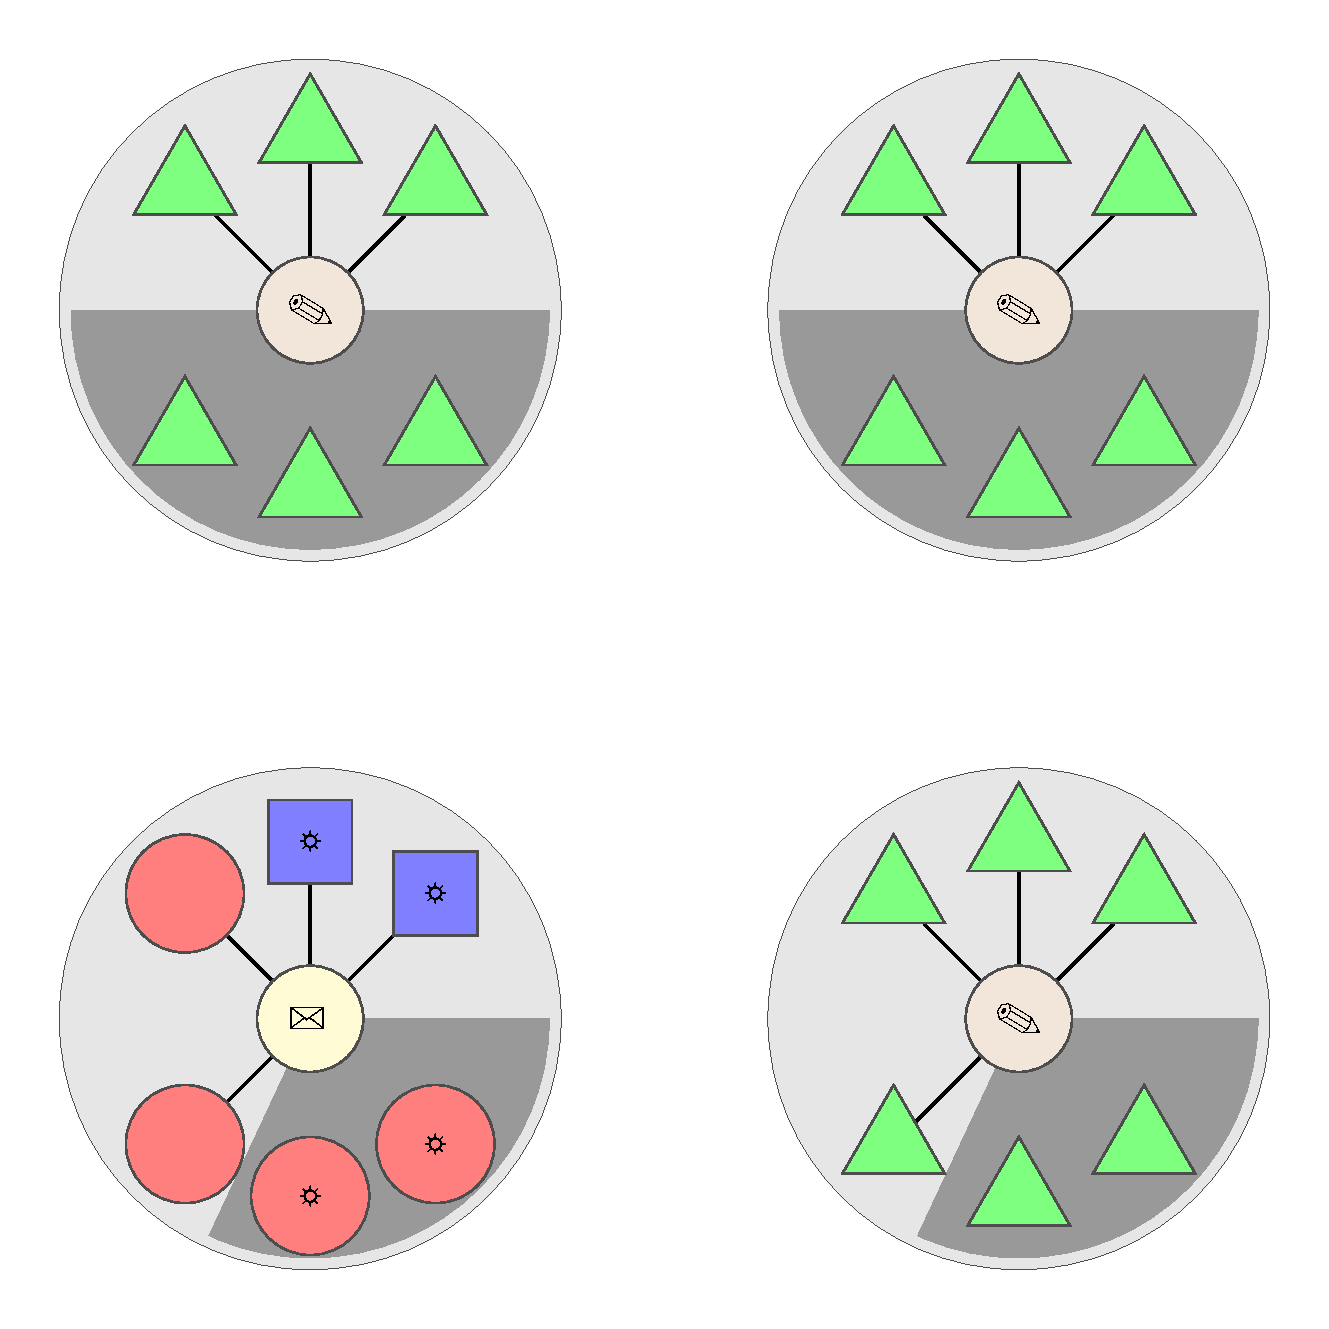
\includegraphics[width=5cm]{pictures/lc_01_4.pdf}}
	    \label{fig:exlc4}
	}
  	\subfloat[][Step 5]{
		\fbox{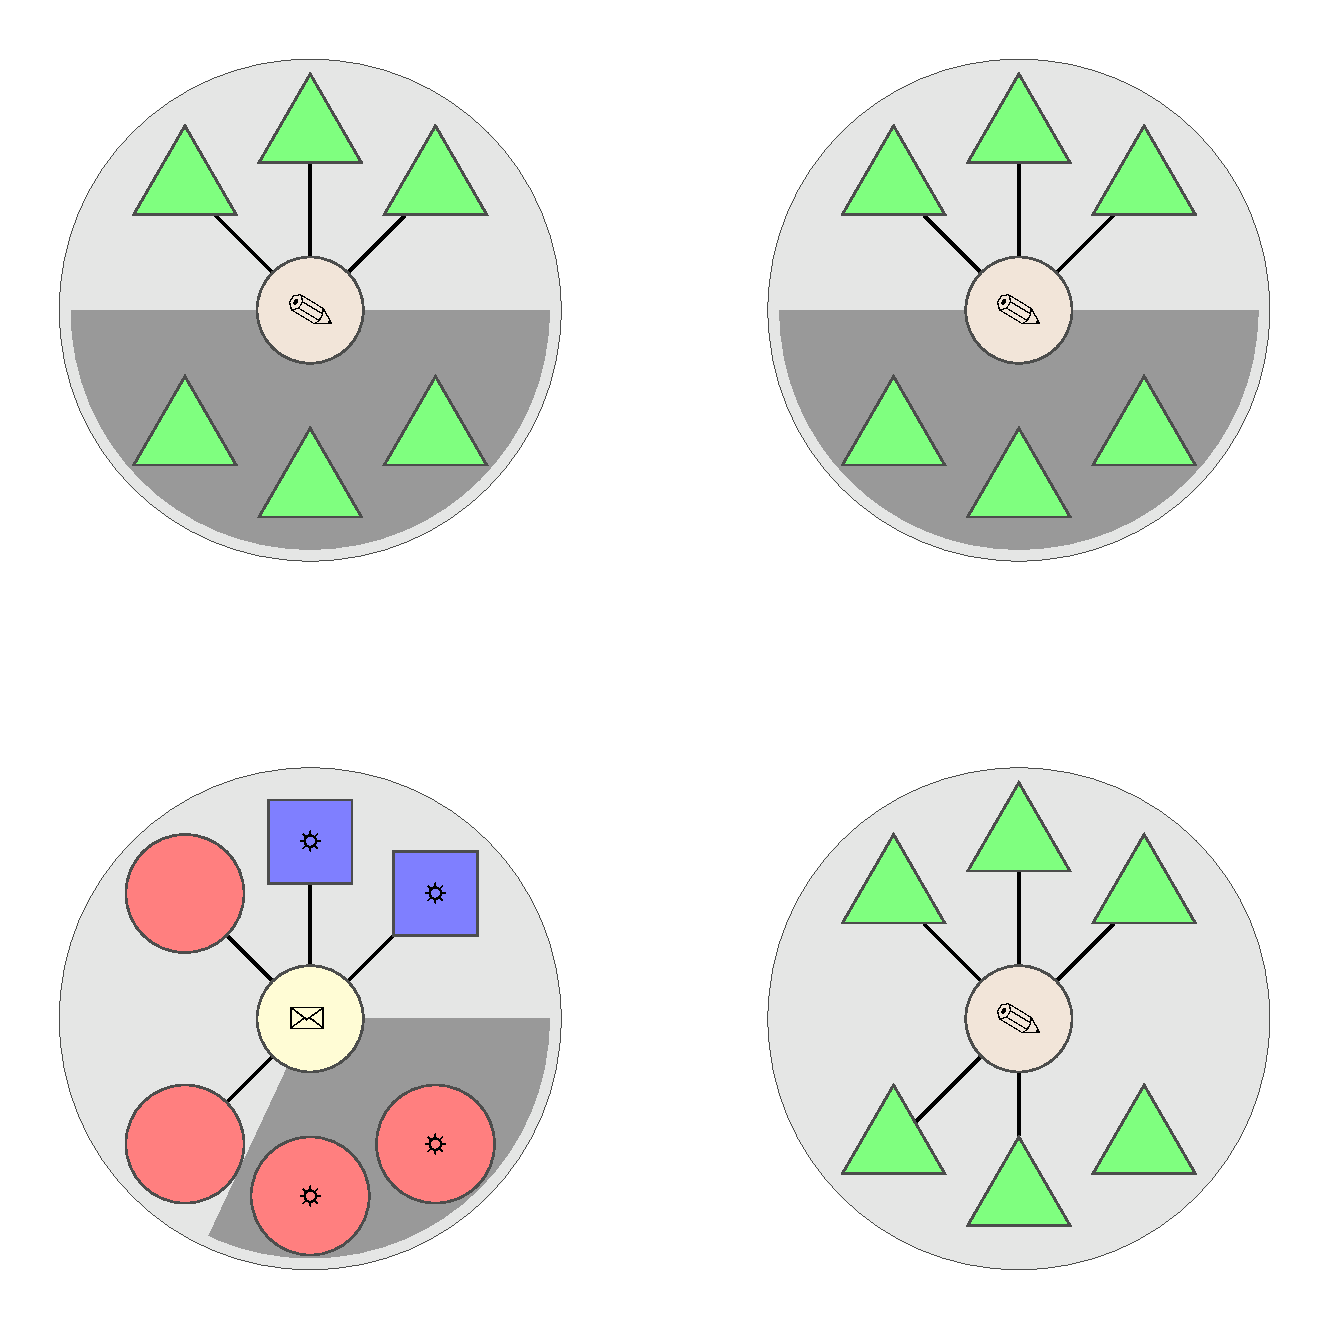
\includegraphics[width=5cm]{pictures/lc_01_5.pdf}}
	    \label{fig:exlc5}
	}
        \\
	\subfloat[][Step 6 (\ec false)]{
		\fbox{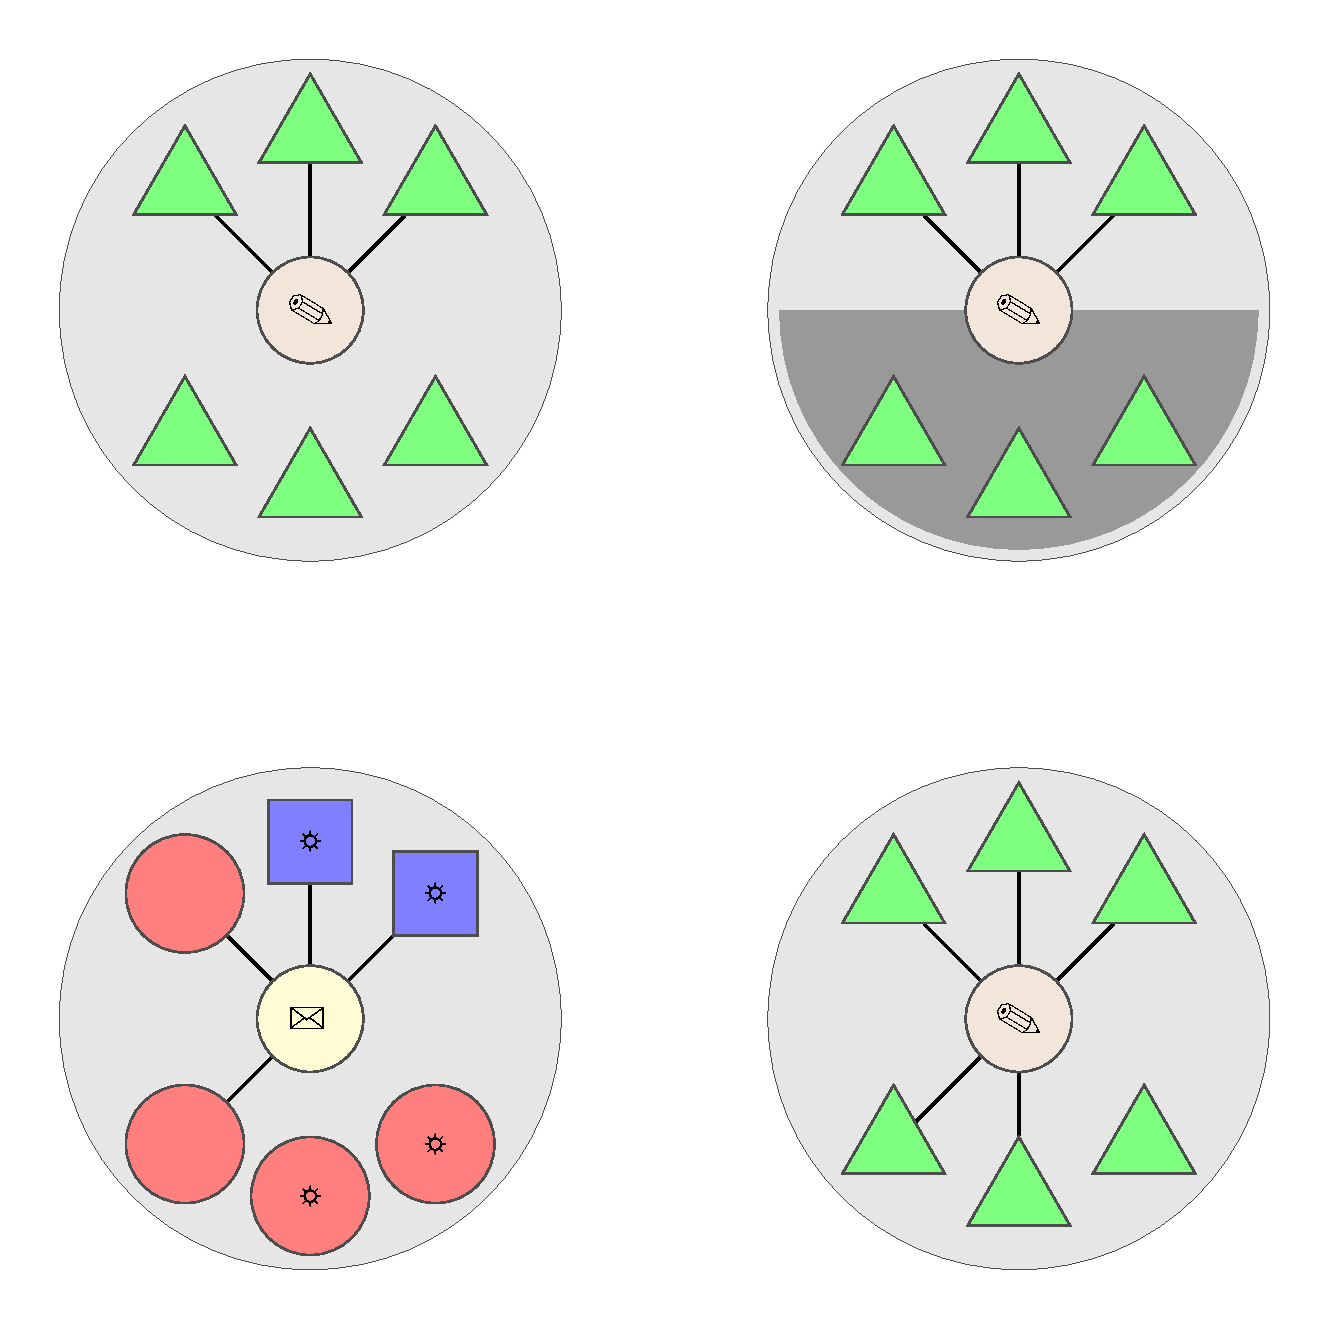
\includegraphics[width=5cm]{pictures/lc_01_6.pdf}}
	    \label{fig:exlc6}
	}
	\subfloat[][Step 7]{
		\fbox{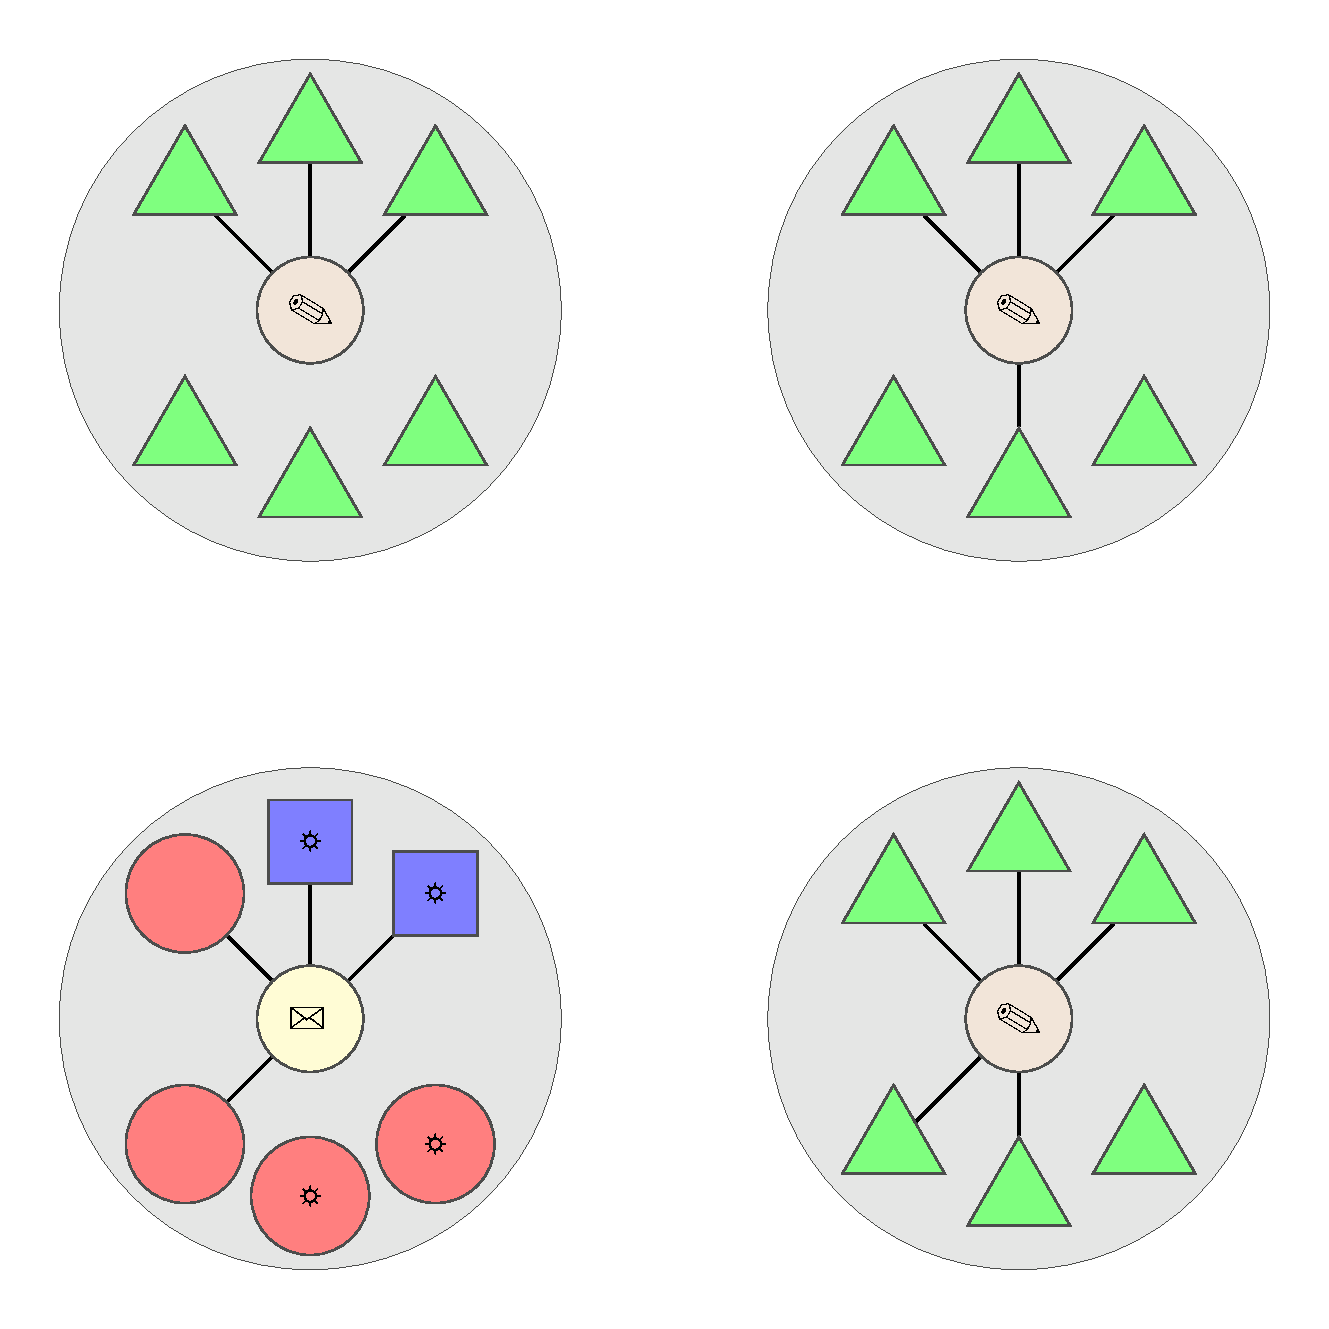
\includegraphics[width=5cm]{pictures/lc_01_7.pdf}}
	    \label{fig:exlc7}
	}
	\caption[]{Example of an \lc-sequence for sentence
          (\ref{bsp:target-related}) where the \lc-reading
          (\ref{bsp:target-related-LC}) can be judged first. The first
          step where all connections are covered is omitted.}
	\label{fig:exlc}
\end{figure}
%
and another in which the dispreferred \ec-reading could be judged
first (Figure~\ref{fig:exec}).
%
\begin{figure}[]
	\centering
	\subfloat[][Step 2]{ 
		\fbox{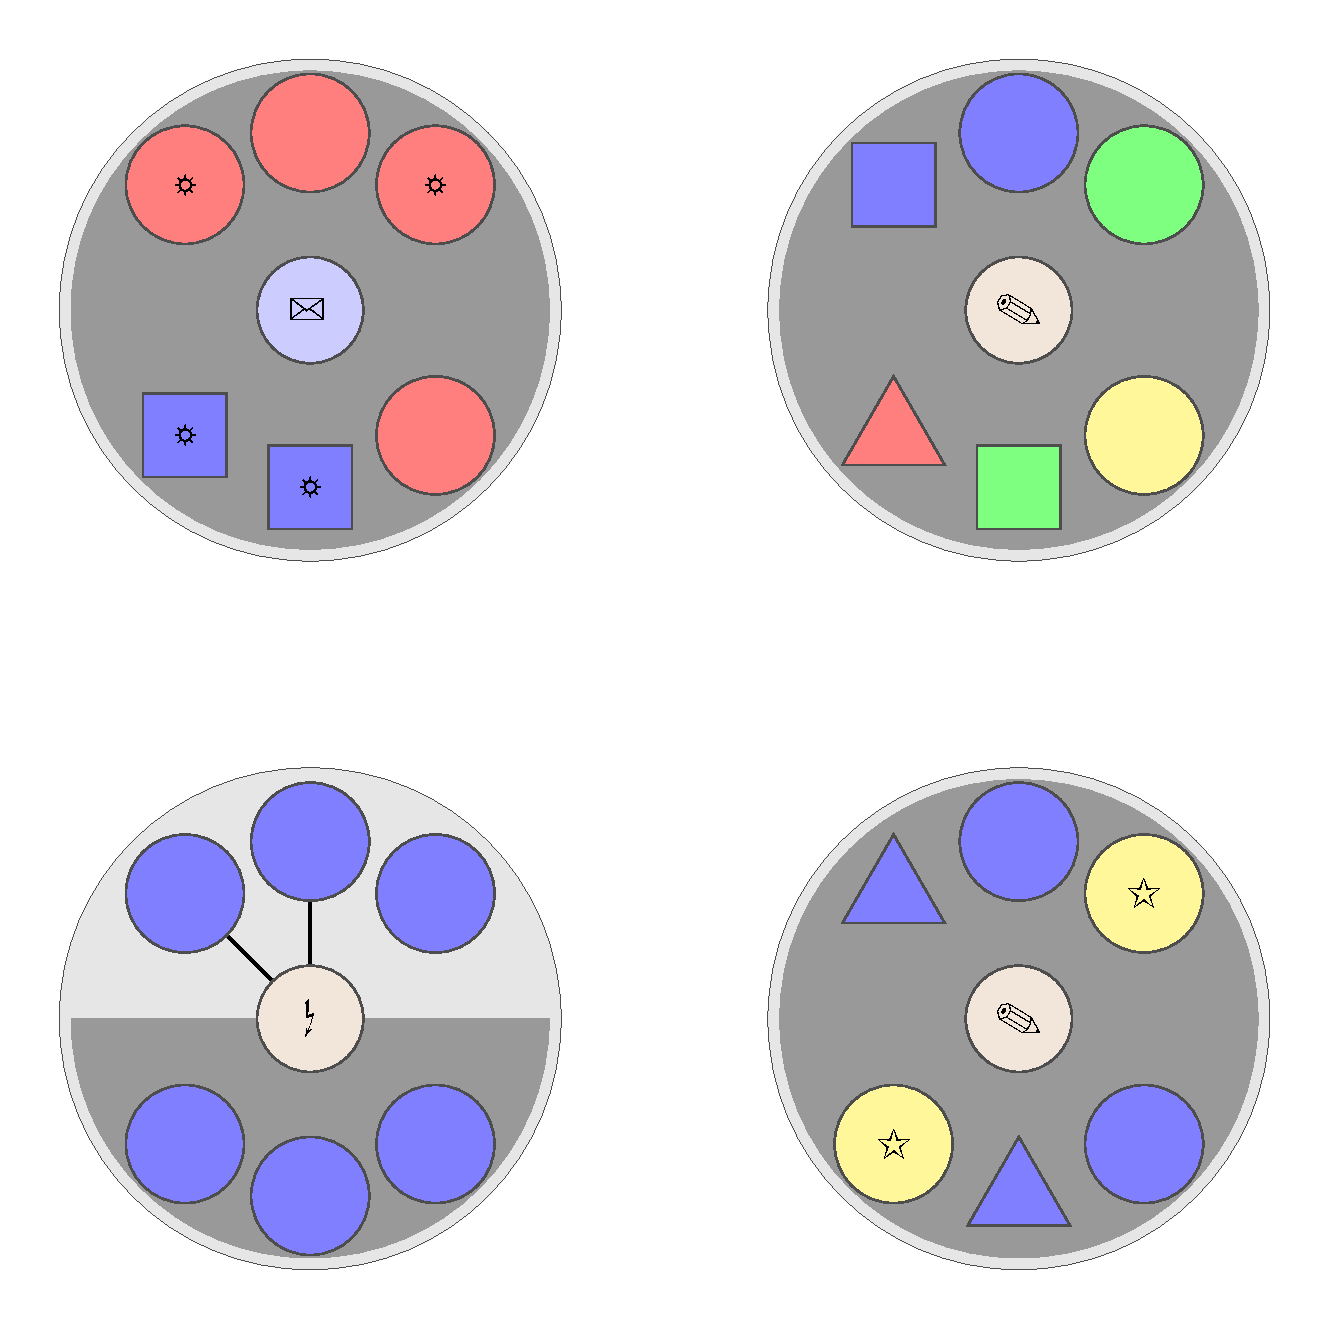
\includegraphics[width=5cm]{pictures/ec_01_2.pdf}}
	    \label{fig:exec1}
	}
	\subfloat[][Step 3 (\ec false)]{
		\fbox{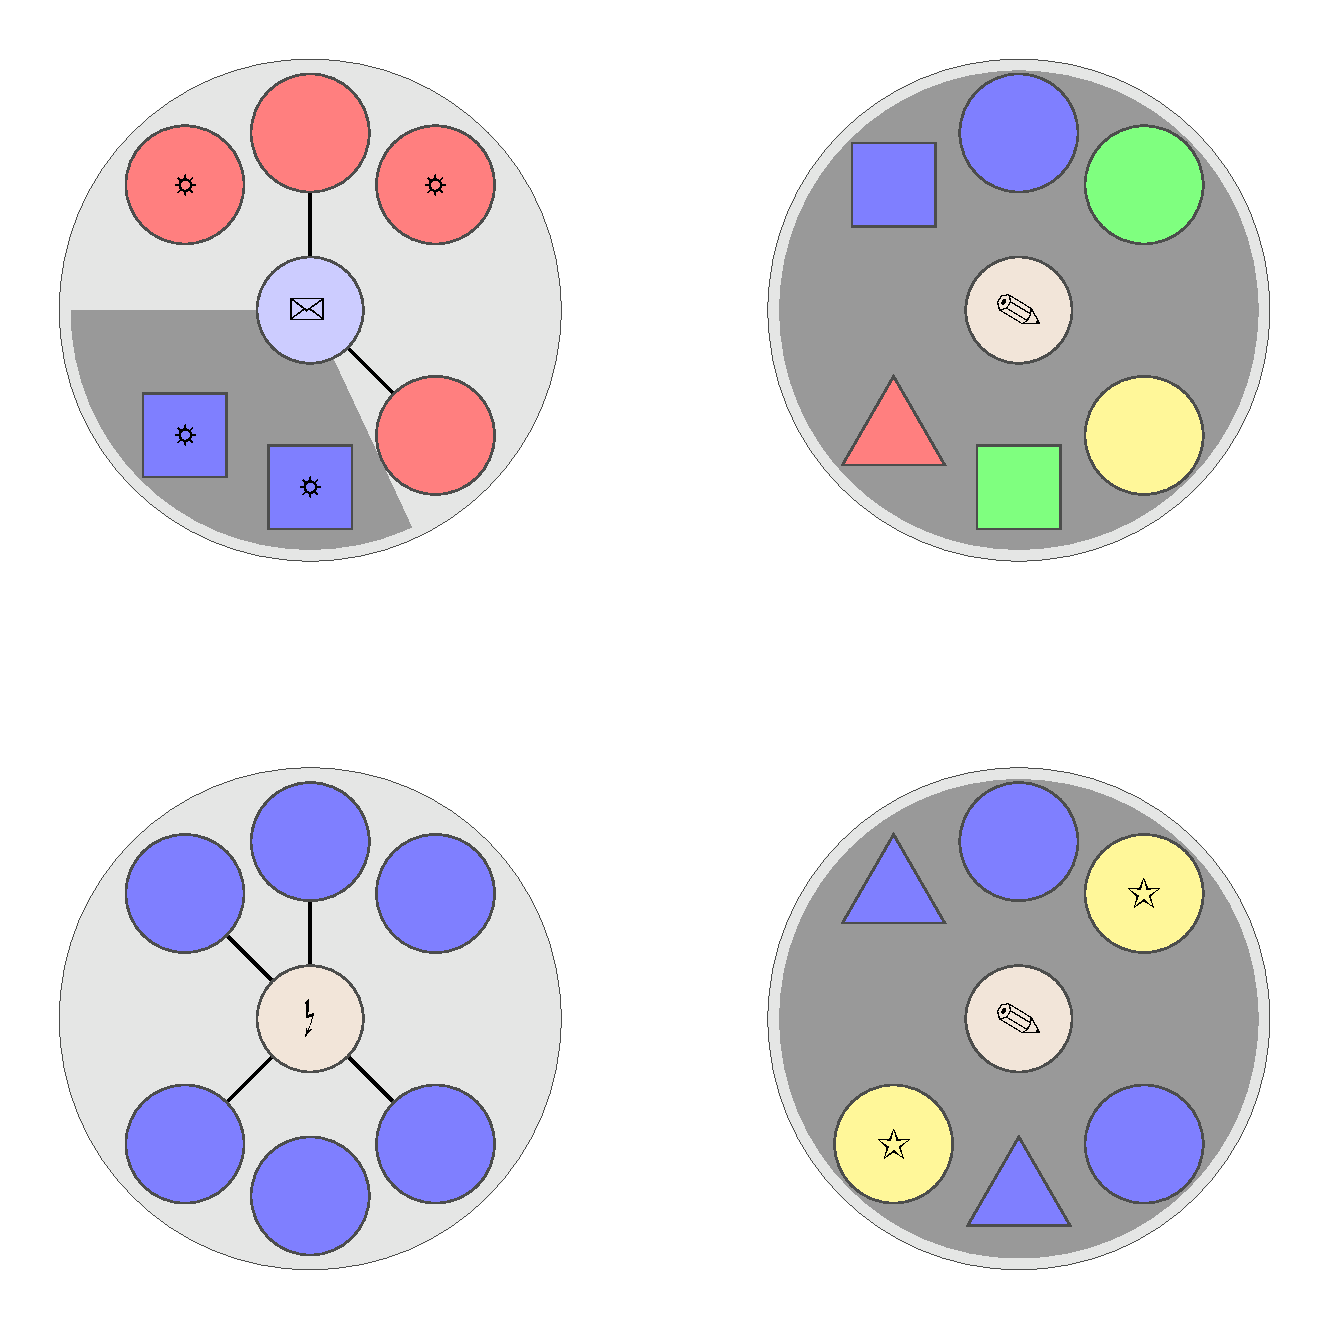
\includegraphics[width=5cm]{pictures/ec_01_3.pdf}}
	    \label{fig:exec2}
	}
        \\
	\subfloat[][Step 4]{
		\fbox{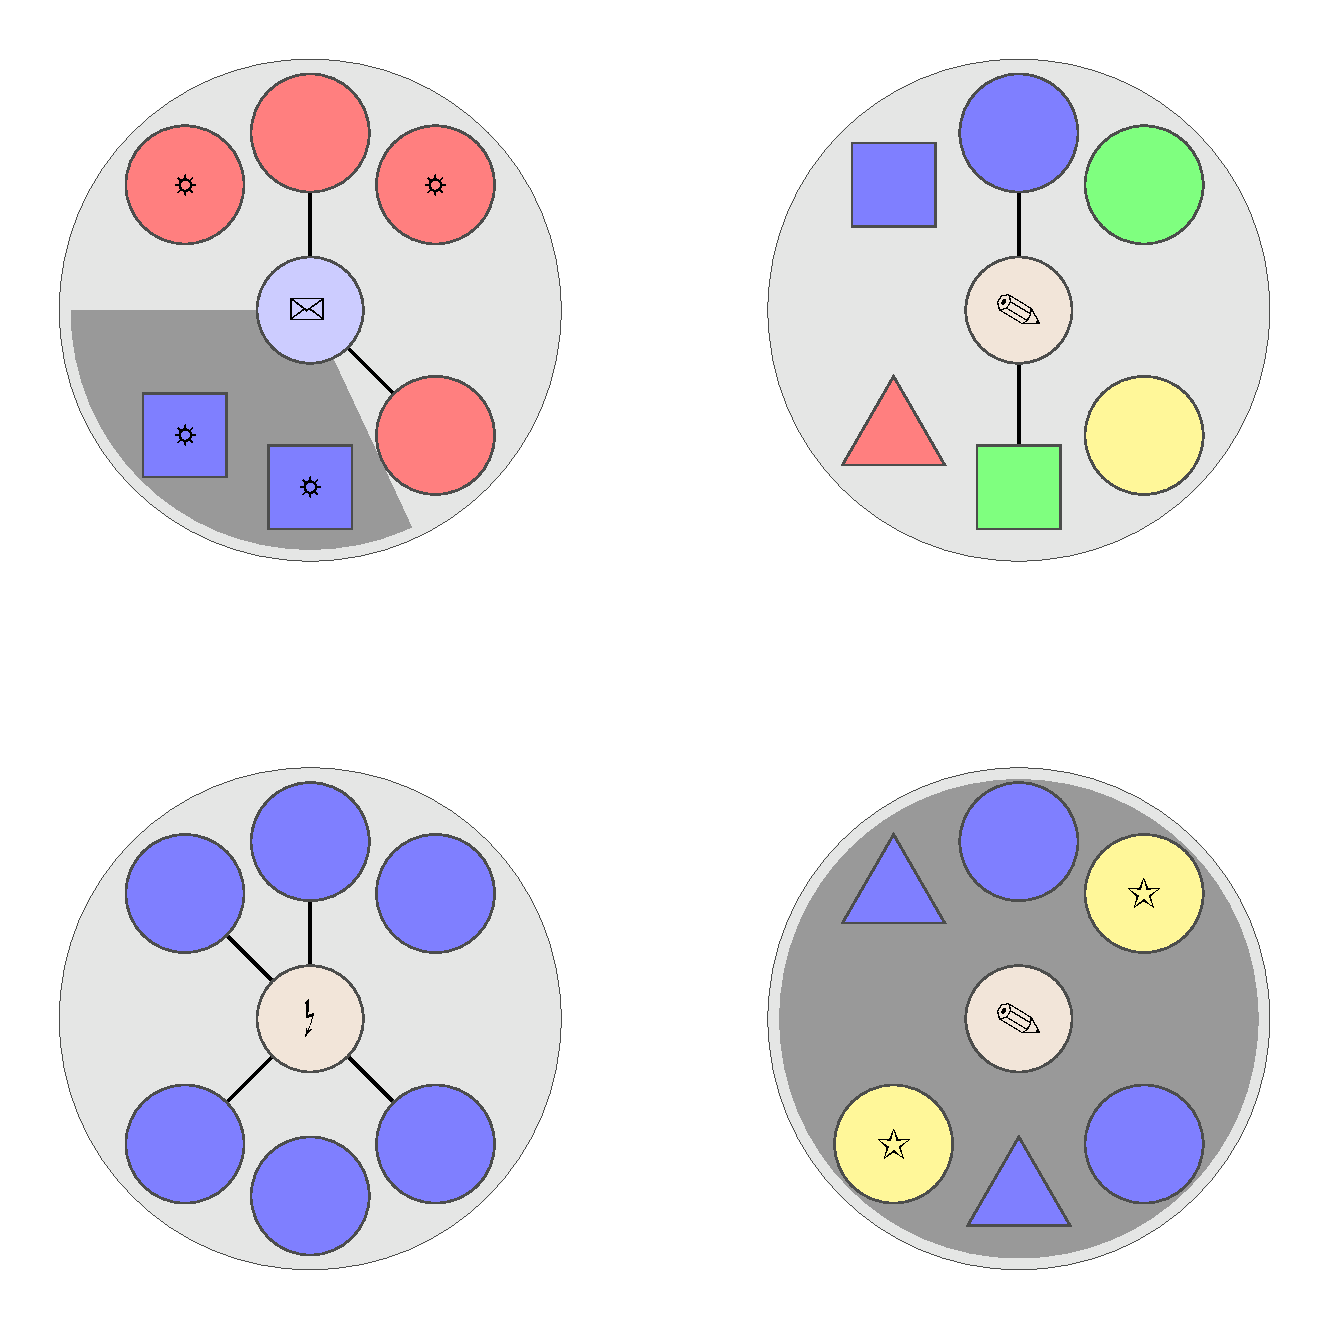
\includegraphics[width=5cm]{pictures/ec_01_4.pdf}}
	    \label{fig:exec2}
	}
	\subfloat[][Step 5 (\lc true)]{
		\fbox{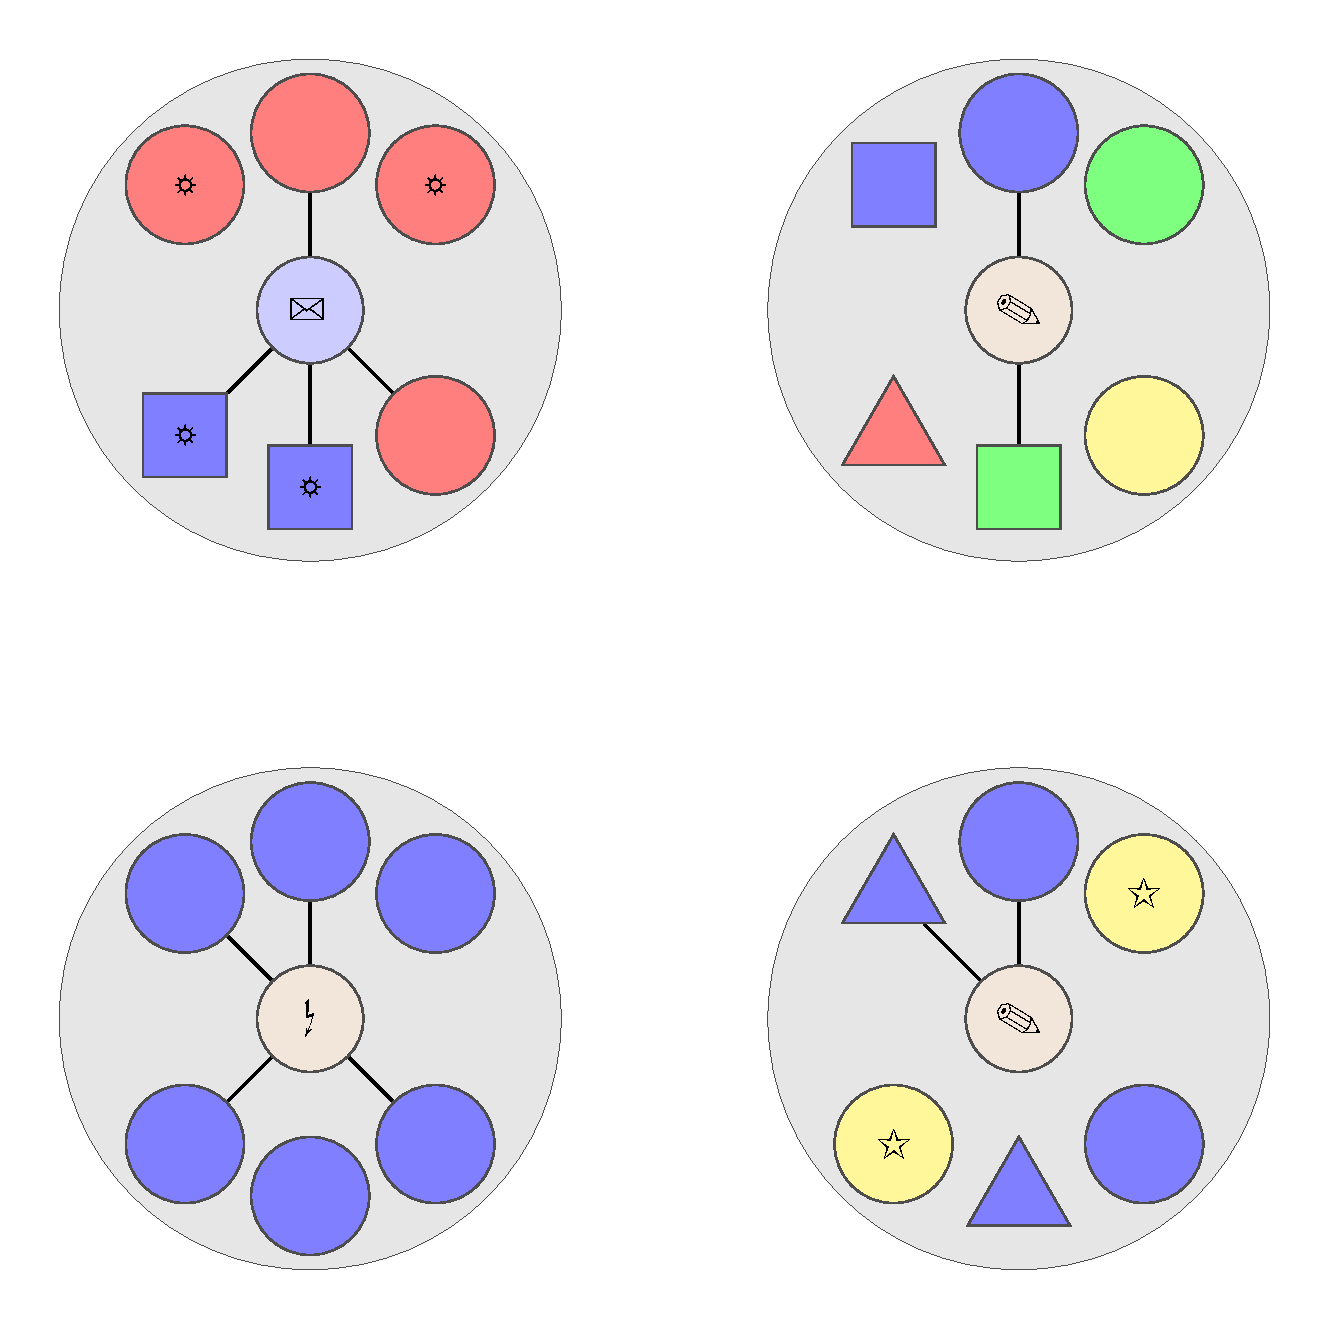
\includegraphics[width=5cm]{pictures/ec_01_5.pdf}}
	    \label{fig:exec2}
	}
	\caption[]{Example of an \ec-sequence for sentence
          (\ref{bsp:target-related}) where the \ec-reading
          (\ref{bsp:target-related-EC}) can be judged first. The first
          step where all connections are covered is omitted.}
	\label{fig:exec}
\end{figure}
%
We also tested structurally disambiguated versions like
(\ref{bsp:target-related2}), one for each sentence type, on each
sequence type for proper comparison.

\begin{exe}

\ex \gll Der Brief ist mit Kreisen, die Sonnen beinhalten, und Vierecken
  verbunden. \label{bsp:target-related2}\\
The letter is with circles, which suns contain and squares connected.\\
The letter is connected with circles containing suns, and with squares.  

\end{exe}


\paragraph{Testing Effects of prosody.} Whereas contrastive accents
are usually assumed to be realized by a special contour in English
(i.e. L+H*, see \cite{Pierrehumbert90}), the exact phonological
classification of contrast in German is still under debate
\citep[see][]{Uhmann91,Fery93,Grabe98,Toepel06,Sudhoff10}.  Still,
all of these approaches have in common that from an acoustic
perceptive, prosodic prominence of contrastively accented constituents
is realized by

\begin{enumerate}[(i)]
\item a higher F0 maximum or a higher pitch range (difference 
between minimal and maximal F0 values), and
\item a longer duration of the accented element as opposed to its 
non-accented counterpart.
\end{enumerate}

\noindent Our sentences were read by a phonetically trained female
native speaker of German familiar with the concept of contrastive
focus. Both \as-sentences and \es-sentences were recorded in two
versions each. In the accented version, a contrastive stress was
placed on {\it einige}. The second version had neutral prosody.  If
accentuation is the driving force for local readings, we would expect
a higher proportion of local readings in the former than in the latter
version of the sentences.

Preference-related controls also differed prosodically. Modifier
attachment ambiguities have been shown to be sensitive to differences
in prosodic phrasing. Though there has been discussion as to whether
speakers reliably \textit{produce} disambiguating cues in such
constructions
\citep[e.g.][]{Allbritton96,Schafer00,Snedeker03,Kraljik05}, overt
prosodic boundaries are generally acknowledged to guide interpretive
processes of attachment ambiguities in \textit{comprehension}
\citep[e.g.][]{Beach1991,KjelgaardSpeer1999,Steinhauer99,SchaferSpeerWarrenWhite2000,CliftonCarlsonFrazier2002,Augurzky06}.
Specifically, it has been shown that prosodically separating a
modifier from the directly preceding material supports an \ec-reading,
whereas separating the two potential attachment sites is supportive of
an \lc-reading
\citep[e.g.][]{CliftonCarlsonFrazier2002,Fodor02,Jun2003}.  Thus, a
phrase boundary between {\it squares} and {\it with} in
(\ref{bsp:target-related}) supports an \ec-reading, whereas a prosodic
phrase boundary following {\it circles} supports an \lc-reading.

To test whether prosodic information could generally have an effect on
answer patterns in our task, we presented sentences in both of these
prosodic variants. In addition, in order to test prosody-independent
preferences, we also included a neutral version without any pronounced
boundary. Further, we also presented unambiguous sentences
corresponding to the \ec-reading. As in the case of the \as- and
\es-sentences, the unambiguous counterparts served as a baseline to
control for response biases that are independent of sentence meaning.





\subsection{Methods}
\label{sec:materials}

\subsubsection{Procedure}
\label{sec:procedure} 

Each experimental trial proceeded as described above. The sentence was
presented using active PC loudspeakers and the picture materials were
presented on a computer screen. Participants responded using the
keyboard. By pressing one of four buttons they could (i) listen to the
sentence (up to three times), (ii) request additional pictorial
information, (iii) respond ``yes, fits'' or (iv) ``no, does not fit''
(German: ``passt'' or ``passt nicht''). At the beginning of an
experimental session participants received written instructions on
their task. Then they completed an interactive training consisting of
15 trials in which they were familiarized with the task.  After the
training the actual experiment started. Participants were tested
individually in a silent room. Each session was divided into two
blocks and participants were told that they could take breaks between
blocks. In total, an experimental session took about one hour. At the
end of the session participants received 8 euros compensation.

\subsubsection{Materials}

\paragraph{Target sentences and positional controls.}

We constructed a set of 15 items for German \as- and \es-sentences,
respectively, analogous to the examples in (\ref{ex:as}) and
(\ref{ex:es}). Sentences were introduced by a subject {\acro{dp}},
including the quantifiers {\it alle diese} ("all of these") or {\it
  genau eine(r) der} ("exactly one of these"), as well as the head
noun which denoted different icons, such as letters or bells. Subject \acros{DP}
were followed by an auxiliary, and a \acro{pp} containing {\it
  einige}, a possessive pronoun, and a noun denoting a geometrical
object, e.g., {\it einigen seiner Dreiecke/Quadrate} ("some of its
triangles/squares"). The possessive pronoun was used in order to fix
relative quantifier scope to surface scope, thus ensuring that {\it
  einige} has embedded status. The last word was the main verb {\it
  verbunden} ("connected").  Each sentence was recorded in a stressed
and an unstressed version of scalar {\it einige}. As described above,
three control sentences were created for each experimental item,
corresponding to the critical positions in the course of uncovering
the accompanying sequences.  The positional controls were recorded
with neutral prosody.  Items were evenly distributed across 5 lists
using a Latin square design.


\paragraph{Preference-related control sentences.}
For controlling preferences, 30 sentences that were ambiguous between
a \lc and an \ec-reading, as well as 30 of their disambiguated
counterparts were constructed as described above. In these sentences,
subject \acros{dp} were always denoting icons and were followed by an
auxiliary. In the ambiguous sentences, the auxiliary was followed by
two {\it with}-\acros{pp} (German: ``mit'').  The first of these
\acros{pp} consisted in a coordination of two nouns denoting
geometrical objects, whereas the nouns in the second \acro{pp} denoted
icons. In contrast to these sentences, the unambiguous sentences
contained only one \acro{pp} with a conjunction the first part of
which was modified by a relative clause.

\paragraph{Acoustic properties.}
% A phonetically trained female native speaker of German was instructed
% to realize two prosodic versions of each target sentence, and three
% versions of the ambiguous preference-related controls. In addition to
% these sentences, the unambiguous preference-related controls, the
% positional controls and a set of unrelated fillers were also
% recorded. For these constructions, the speaker was instructed to
% realize prosodic contours as neutral and natural as possible.

For all target sentences (\as and \es), the determiner \emph{einige} was
produced with a contrastive pitch accent as well as with a neutral
accent. % Contrastive accents in German are realized by an increase in F0 (range)
% as well as by a longer duration (see Section~\ref{sec:design} above). 
A set of 15 
experimental items was recorded for each condition (\as vs.~\es, \emph{accented} 
vs.~\emph{unaccented}), resulting in a total number of 60 target sentences.

In contrast to the accent manipulation, the ambiguous
preference-related controls differed with respect to prosodic
phrasing. Prosodic phrase boundaries in German are realized by a rise
in F0 as well as by a durational increase on the final part of the
constituent preceding the boundary (prefinal lengthening) plus an
optional pause \citep[e.g.][]{Vaissiere83,Fery93}.  Boundaries for
these control sentences were either realized at the position
separating the second \acro{pp} from the preceding material
(\emph{late boundary}, corresponding to an \ec-reading) or directly
preceding the second conjunct in the first \acro{pp} (\emph{early
  boundary}, corresponding to an \lc-reading). As the prosodic
realization of the targets involved the comparison between an accented
and a neutral variant, we also included a third version of the
ambiguous preference-related controls without any pronounced
boundaries. For each prosodic variant, a set of 30 items was read,
yielding 90 preference-related controls.

Altogether a total number of 300 sentences consisting of 60 target
sentences, 90 ambiguous preference-related controls, 30 unambiguous
preference-related controls, 90 positional control sentences and 30
unrelated fillers was recorded. The session was recorded in an
acoustically shielded booth (44.1\,kHz sampling rate, 16 bit amplitude
resolution).

Before entering the judgment task, experimental items and
preference-related controls were analyzed with respect to their acoustic
properties. As both accented elements as well as prosodic boundaries
were expected to differ with respect to their F0 and/or durational
properties, we calculated durational values as well as difference
values between minimal and maximal F0 for each word. Since targets
slightly differed with respect to the total number of words as well as
with respect to certain lexical properties (i.e., \emph{seinen}
vs.~\emph{ihren}, we considered the following analysis regions:

\begin{exe}
  \ex
    \begin{xlist}
      \ex $|_{\text{R}1}$~Alle  	\ $|_{\text{R}2}$~diese 
      \ $|_{\text{R}3}$~$\acro{np}_1$  
      \ $|_{\text{R}4}$~sind  \ $|_{\text{R}5}$~mit  \
      $|_{\text{R}6}$~einigen  \ $|_{\text{R}7}$~ihrer 
       \ $|_{\text{R}8}$~{$\acro{np}_2$}  \ $|_{\text{R}9}$~verbunden.
    \ex       $|_{\text{R}1}$~Genau einer  	\ $|_{\text{R}2}$~der 
      \ $|_{\text{R}3}$~$\acro{np}_1$  
      \ $|_{\text{R}4}$~ist  \ $|_{\text{R}5}$~mit  \
      $|_{\text{R}6}$~einigen  \ $|_{\text{R}7}$~seiner 
       \ $|_{\text{R}8}$~{$\acro{np}_2$}  \ $|_{\text{R}9}$~verbunden.
    \end{xlist}
    % \begin{tabbing}
    %   $|_{\text{R}1}$ Genau einer \= 	\ $|_{\text{R}2}$ diese \=
    %   \ $|_{\text{R}3}$ \acro{np}$_1$ \= 
    %   \ $|_{\text{R}4}$ sind \= \ $|_{\text{R}5}$ mit \= \
    %   $|_{\text{R}6}$ einigen \= \ $|_{\text{R}7}$ seiner 
    %   \= \ $|_{\text{R}8}$  \acro{np}$_2$ \= \ $|_{\text{R}9}$
    %   verbunden. \kill
    %   $|_{\text{R}1}$ Alle \> 	\ $|_{\text{R}2}$ dieser \>
    %   \ $|_{\text{R}3}$ \acro{np}$_1$ \> 
    %   \ $|_{\text{R}4}$ sind \> \ $|_{\text{R}5}$ mit \> \
    %   $|_{\text{R}6}$ einigen \> \ $|_{\text{R}7}$ ihrer 
    %   \> \ $|_{\text{R}8}$  \acro{np}$_1$ \> \ $|_{\text{R}9}$
    %   verbunden. \\
    %   $|_{\text{R}1}$ Genau einer \> 	\ $|_{\text{R}2}$ der \>
    %   \ $|_{\text{R}3}$ \acro{np}$_1$ \> 
    %   \ $|_{\text{R}4}$ ist \> \ $|_{\text{R}5}$ mit \> \
    %   $|_{\text{R}6}$ einigen \> \ $|_{\text{R}7}$ seiner 
    %   \> \ $|_{\text{R}8}$  \acro{np}$_1$ \> \ $|_{\text{R}9}$ verbunden.
    % \end{tabbing}
\end{exe}

\noindent Note that differences between Regions 1, 2, 4 and 7 can be expected
due to lexical differences between the \as and \es-conditions. As
preference-related controls did not differ with respect to their lexical
properties, we carried out word-by-word analyses for these
conditions. Durational values included the respective word plus any
following silent interval. We did not include the
disambiguated fillers in these analyses as they involved very
different sentence types (i.e., constructions involving prepositional
phrases vs.~relative clauses).

\begin{exe}
  \ex $|_{\text{R}1}$ \acro{D}  	\ $|_{\text{R}2}$ $\acro{np}_1$
      \ $|_{\text{R}3}$ ist 
      \ $|_{\text{R}4}$ mit  \ $|_{\text{R}5}$ $\acro{np}_2$   \
      $|_{\text{R}6}$ und  \ $|_{\text{R}7}$ $\acro{np}_3$ 
       \ $|_{\text{R}8}$  mit  \ $|_{\text{R}9}$ $\acro{np}_4$ \ $|_{\text{R}10}$~verbunden.
\end{exe}

For the durational analyses, constituents were automatically labeled
by the \emph{Aligner} tool \citep{Rapp98}, and the
obtained values were manually corrected afterwards. For the targets,
two-factorial \acros{anova} with the factors \acro{Quantifier} (\emph{all}
vs.~\emph{exactly one}) and \acro{Prosody} (accented vs.~unaccented) were
carried out. For the preference-related controls, we carried out
one-factorial \acros{anova} with the factor \acro{Prosody} (early
boundary, late boundary, neutral prosody). F0 values were extracted by
means of special Praat scripts
(\url{http://www.fon.hum.uva.nl/praat/}). For the present analyses,
differences between minimal and maximal F0 values for each region or
word were calculated. Again, two-factorial \acros{anova} were carried
out for statistical comparison of the target sentences, and one-factorial
\acros{anova} were carried out for preference-related controls.


\paragraph{Targets.} 
Differences between maximal and minimal F0 values for each of the
single words in the sentence are depicted in
Figure~\ref{fig:minmax_targets}. As expected, accented
determiners showed a larger F0 range compared to unaccented versions,
an effect which was confirmed by statistical analyses (effects on
the determiner: \acro{Prosody}: \emph{F}=94.8; \emph{p}<.001); 
Interaction of \acro{Quantifier} and \acro{Prosody}: \emph{F}=13.7; 
\emph{p}<.01). The observed interaction indicates that these differences
are even more pronounced in the \as-condition.

\begin{figure}[]
	\centering
	\subfloat[][\as-sentences]{
          \begin{tikzpicture}[scale=0.75]
  \begin{axis}[
    cycle list name = mylist,
    legend pos = north west,
    ymajorgrids,
    ymax = 250,
    y = 0.5,
    x tick label style = {rotate = 50, anchor = east},
    xtick = data,
    xticklabels = {alle,diese,N1,sind,mit,einigen,ihrer,N2,verbunden}
    ]
    \addplot+[line width = 1.3pt] coordinates {
      (0 ,17.6)
      (1 ,27.4)
      (2 ,82.6)
      (3 ,32.6)
      (4 ,62.4)
      (5 ,211.3333333)
      (6 ,57.6)
      (7 ,36.66666667)
      (8 ,47.13333333)};

  \addplot+[line width = 1.3pt] coordinates {
        (0 ,19.6        )
        (1 ,36.46666667 )
        (2 ,115.1333333 )
        (3 ,60.6        )
        (4 ,46          )
        (5 ,69.86666667 )
        (6 ,46.66666667)
        (7 ,71.4)
        (8 ,61.46666667)};

      \legend{accented, neutral}
  \end{axis}
\end{tikzpicture}
		% \fbox{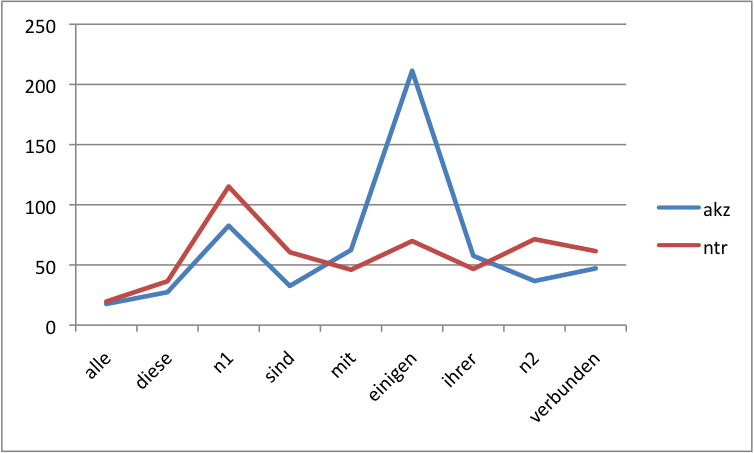
\includegraphics[width=5.5cm]{pictures/paper/minmax_ae.png}}
	    \label{fig:minmax_ae}
	}
	\subfloat[][\es-sentences]{
\begin{tikzpicture}[scale=0.75]
  \begin{axis}[
    cycle list name = mylist,
    legend pos = north west,
    ymajorgrids,
    ymax = 250,
    y = 0.5,
    x tick label style = {rotate = 50, anchor = east},
    xtick = data,
    xticklabels = {genau,einer,dieser,N1,ist,mit,einigen,seiner,N2,verbunden}
    ]
    \addplot+[line width = 1.3pt] coordinates {
        (     0 , 59.06666667 )
        (     1 , 46.26666667 )
        (     2 , 19          )
        (     3 , 67.6        )
        (     4 , 17.6        )
        (     5 , 39.8        )
        (     6 , 174.9333333 )
        (     7 , 30.46666667 )
        (     8 , 32.46666667 )
        (     9 , 42.33333333 )};

  \addplot+[line width = 1.3pt] coordinates {
        (0 , 30.21428571 )
        (1 , 34.21428571 )
        (2 , 17.07142857 )
        (3 , 93.78571429 )
        (4 , 28.64285714 )
        (5 , 67.64285714 )
        (6, 75.5        )
        (7 , 25.71428571 )
        (8 , 54.85714286 )
        (9 , 55)};

      \legend{accented, neutral}


  \end{axis}
\end{tikzpicture}
		% \fbox{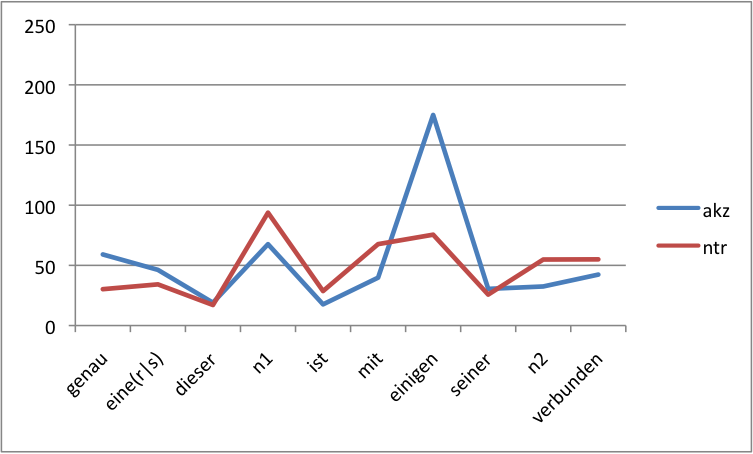
\includegraphics[width=5.5cm]{pictures/paper/minmax_ge.png}}
	    \label{fig:minmax_ge}
	}
	\caption[]{Differences between minimal and maximal F0 values (in Hz) for 
	the single regions for \as-sentences (a) and \es-sentences (b).}
	\label{fig:minmax_targets}
\end{figure}

\begin{figure}[]
	\centering
	\subfloat[][\as-sentences]{ 
\begin{tikzpicture}[scale=0.75]
  \begin{axis}[
    cycle list name = mylist,
    legend pos = north west,
    ymajorgrids,
    ymax = 800,
    ymin = 0,
    y = 0.125,
    x tick label style = {rotate = 50, anchor = east},
    xtick = data,
    xticklabels = {alle,diese,N1,sind,mit,einigen,ihrer,N2,verbunden}
    ]
    \addplot+[line width = 1.3pt] coordinates {
      (0 ,225.8333333)
      (1 , 245.3333333 )
      (2 , 397         )
      (3 , 172.3333333 )
      (4 , 230.1666667 )
      (5 , 445.8333333 )
      (6, 199.6666667)
      (7, 503)
      (8 ,722 )
    };

  \addplot+[line width = 1.3pt] coordinates {
        (0 , 216.9212    )
        (1 , 234.6666667 )
        (2 , 414.6666667 )
        (3 , 175.5       )
        (4 , 170.5       )
        (5 , 422         )
        (6 , 194.6666667 )
        (7 , 494.6666667 )
        (8 , 748)
};

      \legend{accented, neutral}


  \end{axis}
\end{tikzpicture}
		% \fbox{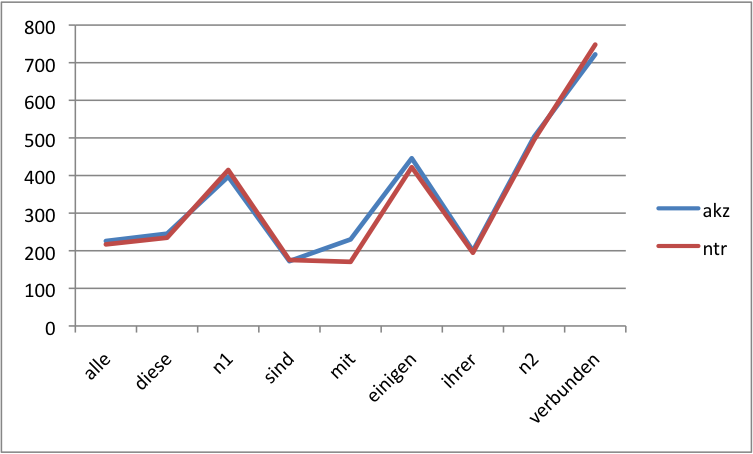
\includegraphics[width=5.5cm]{pictures/paper/duration_ae.png}}
	    \label{fig:duration_ae}
	}
	\subfloat[][\es-sentences]{
          \begin{tikzpicture}[scale=0.75]
  \begin{axis}[
    cycle list name = mylist,
    legend pos = north west,
    ymajorgrids,
    ymax = 800,
    ymin = 0,
    y = 0.125,
    x tick label style = {rotate = 50, anchor = east},
    xtick = data,
    xticklabels = {genau,einer,dieser,N1,ist,mit,einigen,seiner,N2,verbunden}
    ]
    \addplot+[line width = 1.3pt] coordinates {
(       0 , 307         )
(       1 , 256         )
(       2 , 128.6666667 )
(       3 , 398.6666667 )
(       4 , 164.6666667 )
(       5 , 226.6666667 )
(       6 , 420.6666667 )
(       7 , 235.3333333 )
(       8 , 494.6666667 )
(       9 , 704.6666667 )
    };

  \addplot+[line width = 1.3pt] coordinates {
(0 , 285.8333333 )
(1 , 244.6666667 )
(2 , 128         )
(3 , 400         )
(4 , 152.6666667 )
(5 , 170         )
(6 , 383.3333333 )
(7 , 249.3333333 )
(8 , 494.6666667 )
(9 , 764.6666667 )
};

      \legend{accented, neutral}


  \end{axis}
\end{tikzpicture}
		% \fbox{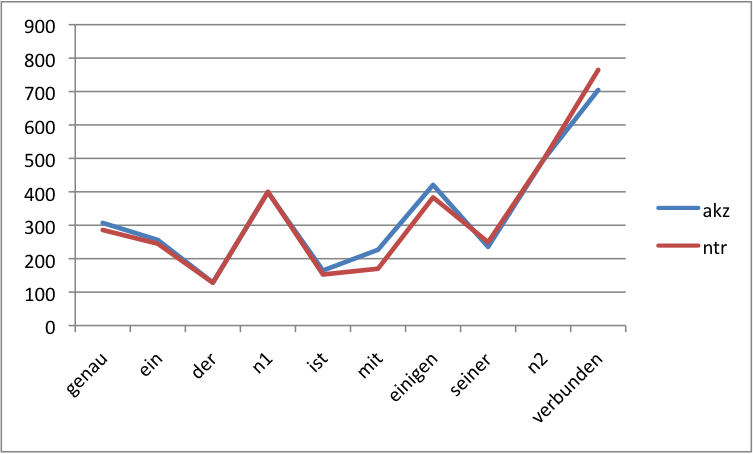
\includegraphics[width=5.5cm]{pictures/paper/duration_ge.png}}
	    \label{fig:duration_ge}
	}
	\caption[]{Durational values (in ms) for 
	the single regions for \as-sentences (a) and \es-sentences (b).}
	\label{fig:duration_targets}
\end{figure}



Figure~\ref{fig:duration_targets} shows the durational values for each
of the single regions in the sentence.  Though descriptively small,
the duration of accented determiners was significantly increased as
opposed to their non-accented counterparts (effects on the determiner:
\acro{Quantifier}: \emph{F}=31.4; \emph{p}<.001; \acro{Prosody}:
\emph{F}=23.8; \emph{p}<.001).  A list of the statistical results of
each sentential region is provided in
Appendix~\ref{sec:audit-sent-mater} (F0 values:
Table~\ref{tab:table-B}; durational values: Table~\ref{tab:table-A}).


\paragraph{Preference-related controls.} 
Differences between maximal and minimal F0 values for each of the
single words in the sentence as well as durational values are depicted in
Figure~\ref{fig:acoustics_fi}. As is
evident, the largest durational and F0 differences were
realized at the boundary regions (i.e. Region 5 and Region
7). 

\begin{figure}[t]
	\centering
	\subfloat[][F0 values]{ 
\begin{tikzpicture}[scale=0.75]
  \begin{axis}[
    cycle list name = mylist,
    legend pos = north west,
    ymajorgrids,
    ymax = 250,
    ymin = 0,
    y = 0.55,
    x tick label style = {rotate = 50, anchor = east},
    xtick = data,
    xticklabels = {D1,N1,ist,mit,N2,und,N3,mit,N4,verbunden}
    ]
    \addplot+[line width = 1.3pt] coordinates {
(       0 ,27.65517241 )
(       1 ,91.20689655 )
(       2 ,32.51724138 )
(       3 ,27.20689655 )
(       4 ,53.72413793 )
(       5 ,19.5862069  )
(       6 ,210.8965517 )
(       7 ,15.48275862 )
(       8 ,66.06896552 )
(       9 ,68.72413793 )
    };

  \addplot+[line width = 1.3pt] coordinates {
(0 ,23.48148148) 
(1 ,63.07407407) 
(2 ,13.7037037 ) 
(3 ,22.7037037 ) 
(4 ,197.0740741) 
(5 ,34.03703704) 
(6 ,95.37037037) 
(7 ,15.22222222) 
(8 ,52.18518519) 
(9 ,123        ) };

  \addplot+[line width = 1.3pt] coordinates {
(0, 31.7        )
(1, 80.2        )
(2, 24.46666667 )
(3, 31.2        )
(4, 135.8333333 )
(5, 54.46666667 )
(6, 86.96666667 )
(7, 16.76666667 )
(8, 51.4        )
(9, 62.53333333 )};

      \legend{\textsc{ec},\textsc{lc},neutral}


  \end{axis}
\end{tikzpicture}
		% \fbox{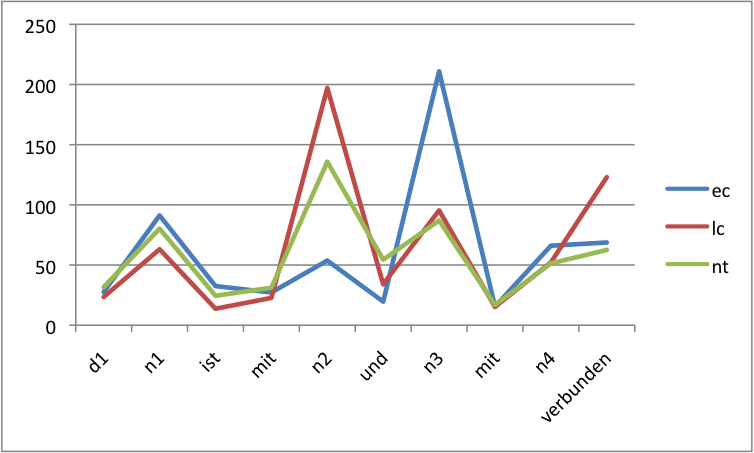
\includegraphics[width=5.5cm]{pictures/paper/minmax_fi.png}}
	    \label{fig:acoustics_fi}
	}
	\subfloat[][Duration]{
\begin{tikzpicture}[scale=0.75]
  \begin{axis}[
    cycle list name = mylist,
    legend pos = north west,
    ymajorgrids,
    ymax = 1400,
    ymin = 0,
    y = 0.1,
    x tick label style = {rotate = 50, anchor = east},
    xtick = data,
    xticklabels = {D1,N1,ist,mit,N2,und,N3,mit,N4,verbunden}
    ]
    \addplot+[line width = 1.3pt] coordinates {
(0  , 105.75      )
(1  , 332.3333333 )
(2  , 168         )
(3  , 135.3333333 )
(4  , 561.3333333 )
(5  , 143.3333333 )
(6  , 1183.666667 )
(7  , 167         )
(8  , 384.6666667 )
(9  , 691.3333333 )
    };

  \addplot+[line width = 1.3pt] coordinates {
(0  , 100.75      )
(1  , 306.6666667 )
(2  , 167         )
(3  , 139.6666667 )
(4  , 1268.333333 )
(5  , 176.3333333 )
(6  , 535.3333333 )
(7  , 150.3333333 )
(8  , 381         )
(9  , 681.3333333 )
};

  \addplot+[line width = 1.3pt] coordinates {
(0  , 98.08333333 )
(1  , 313.6666667 )
(2  , 169.3333333 )
(3  , 141.3333333 )
(4  , 642.6666667 )
(5  , 150         )
(6  , 557.3333333 )
(7  , 151         )
(8  , 402.6666667 )
(9  , 730)
};

      \legend{\textsc{ec},\textsc{lc},neutral}


  \end{axis}
\end{tikzpicture}
		% \fbox{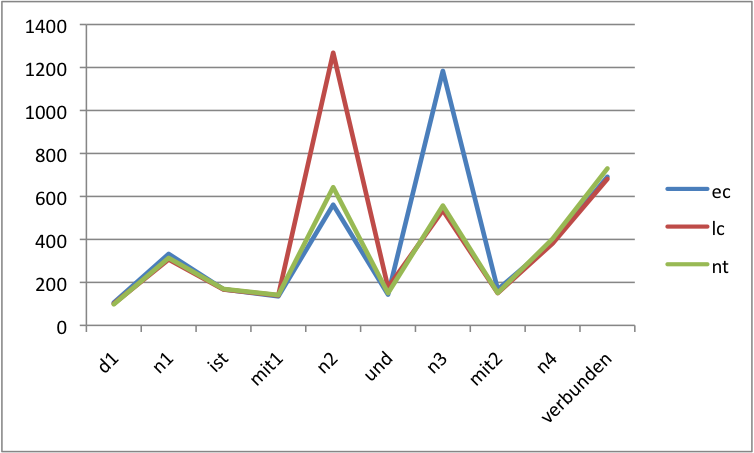
\includegraphics[width=5.5cm]{pictures/paper/duration_fi.png}}
	    \label{fig:duration_fi}
	}
	\caption[]{Differences between minimal and maximal F0 values (in Hz) (a) as well
	as durational values (in ms)(b) for 
	the single regions  .}
	\label{fig:acoustics_fi}
\end{figure}


Statistical analyses for F0 on Region 5 reveal that all prosodic
realizations (\emph{neutral} vs. (\emph{early boundary}
vs. (\emph{late boundary})) differ significantly from each other
(effect of \acro{Prosody}: \emph{F}=129.3; \emph{p}<.001; all single
comparisons \emph{p}<.001). On Region 7, F0 analyses again show a main
effect of \acro{Prosody}: \emph{F}=132.5; \emph{p}<.001. However, the
comparison between neutral prosody and a \emph{late boundary} did not
reach significance (\emph{p}>.2). Finally, durational analyses reveal
that all prosodic realizations (\emph{neutral} vs. (\emph{early
  boundary} vs. (\emph{late boundary})) differ significantly from each
other (Region 5: effect of \acro{Prosody}: \emph{F}=819.5;
\emph{p}<.001; all single comparisons \emph{p}<.001; Region 7: effect
of \acro{Prosody}: \emph{F}=1920.3; \emph{p}<.001; all single
comparisons \emph{p}<.001.) A list of the statistical results of each
sentential region is provided in Appendix~\ref{sec:audit-sent-mater}
(F0 values: Table~\ref{tab:table-D}; durational values:
Table~\ref{tab:table-C}).

In sum, our speaker reliably
produced (i) differences in accent realization for the target
sentences and (ii) the expected boundary realizations for the
preference-related controls. Whereas accented elements clearly
differed from their unaccented counterpart by showing an increase in
duration and F0 range, prosodic boundaries for our preference-related
controls were realized by pre-final lengthening (i.e., an increase in F0
and duration at the position preceding the boundary).


\paragraph{Pictures.}
The visual sequences accompanying each sentence consisted of pictures
like in Figures~\ref{fig:exseqAS}--\ref{fig:exlc}. In each picture,
four alternative sub-scenarios were presented, in which an icon was
surrounded by six geometrical shapes. Depending on the sentence
material, shapes and icons differed across sentence types and
conditions. For example, in our target conditions, 4 identical icons
were surrounded by geometrical shapes that were all of the same type,
whereas various icons and surrounding elements were used in each
sequence of the preference-related control structures (see
Section~\ref{sec:design} for more detailed exposition). Pictures for
unrelated fillers had critical positions at random uncovering stages,
including cases where no uncovering was needed for a truth-value
judgement.

\paragraph{Lists.}
Experimental items and preference-related controls were evenly
distributed across lists. For the \as- and \es-sentences together with
their respective controls, five lists were used employing a Latin
square design. Picture sentence-pairs for the preference-related
controls were spread across eight lists. Each target list was combined
with each list from the preference-related controls, thus yielding to
a total of forty lists. The thirty unrelated filler items were
included in each of these resulting lists.

\subsubsection{Participants.} 

Forty native speakers of German took part in our study, none of whom
had any prior exposure to logic or formal semantics. We excluded two
participants due to insufficient performance on controls ($\le 60\%$
correct answers).

\subsection{Results}
\label{sec:results}

In the following, we will report the results for target conditions and
preference-related controls separately. After providing the
descriptive results, we present statistical analyses using log-linear
models. We complement these with a Bayesian analysis that is sensitive
to the sequential nature of the incremental verification task and
probes specifically into the preference relations between candidate
readings.

\paragraph{Target conditions and positional controls.}
Performance on positional controls was overwhelmingly correct (90\%
correct responses on average with a variance of 0.012) indicating that
participants understood the task and were able to give correct
truth-value judgments at the adequate point in a sequence. In
general, they were not affected by inessential features of the picture
materials or general response biases.

% \begin{figure}[t] 
% \centering

% \includegraphics[width=0.9\textwidth]{positional_answers_critical.pdf}


% \caption{Answers for the \as- and \es-sequences. Bars show the total
%   number of \emph{yes} (up) and \emph{no} judgments (down) collected
%   at each step during a sequence. E.g., we recorded a total of 103
%   \emph{yes} judgments at the third position in the \as-sequence with
%   neutral intonation, which corresponds to 103 answers that were
%   classified as \emph{literal} answers. Notice that the \as-condition
%   had seven steps, the \es-condition only five.}
% \label{fig:JudgmentsK2}
% \end{figure}
%

\begin{table}
  \centering
  \begin{tabular}{lcccccccc@{\hskip 0.6cm}cccc}
    && \multicolumn{7}{c}{truth value at step}
    & \multicolumn{4}{c}{classification}
    \\ \cmidrule(l){3-9} \cmidrule(r){10-13}
    condition &
    & 1
    & 2
    & 3
    & 4
    & 5
    & 6
    & 7
    & \lit
    & \loc
    & \glb
    & err \\ \midrule
    \as-ntr 
    & T & 1 & 1 & \textbf{103} & 2 & \textbf{0} & 0 & 2 
    & 103 & 3 & 0 & 8 \\
    & F & 0 & 0 & 0 & 0 & 2 & 0 & \textbf{3} \\ 
    \addlinespace[0.25cm]
    \as-acc
    & T & 0 & 1 & \textbf{99} & 2 & \textbf{2} & 0 & 1 
    & 99 & 8 & 2 & 5 \\
    & F & 0 & 0 & 1 & 0 & 0 & 0 & \textbf{8} \\
    \addlinespace[0.25cm]
    \es-ntr
    & T & 0 & 11 & 3 & 1 & \textbf{14} & - & - 
    & 78 & 14 & 0 & 22 \\
    & F & 0 & \textbf{0} & \textbf{78} & 5 & 2 & - & - \\
    \addlinespace[0.25cm]
    \es-acc
    & T & 0 & 10 & 3 & 0 & \textbf{16} & - & - 
    & 78 & 16 & 0 & 20 \\
    & F & 0 & \textbf{0} & \textbf{78} & 5 & 2 & - & -
  \end{tabular}
  \caption{Observed truth-value judgments in critical conditions. The
    left-hand part of the table shows the number of \emph{true} and
    \emph{false} responses obtained at each step in the sequence. The
    right-hand part shows the count for our imposed classification
    scheme. The answer counts indicative of relevant readings are
    given in bold-face on the left-hand side.}
  \label{tab:count_data_CC}
\end{table}


%
% \begin{table}[h]
% \centering

% \begin{tabular}{lccccc}
%   condition & position & \multicolumn{4}{c}{response type} \\ \cmidrule(r){3-6}
%   && \emph{literal} & \emph{local} & \emph{global} & \emph{error} \\
%   \midrule \addlinespace[0.15cm]
%   \textbf{\as neutral} 
%   & Pos 1 & 35 &  0 & 0 & 3 \\
%   & Pos 2 & 35 &  1 & 0 & 2 \\
%   & Pos 3 & 33 &  2 & 0 & 3 \\ \addlinespace[0.15cm]
%   & \textbf{Total} & \textbf{103} &  \textbf{3} & \textbf{0} &
%   \textbf{8} \\
%   \addlinespace[0.25cm]
%   \textbf{\as accented} 
%   & Pos 1 & 33 &  2 & 1 & 2 \\
%   & Pos 2 & 33 &  3 & 1 & 1 \\
%   & Pos 3 & 33 &  3 & 0 & 2 \\ \addlinespace[0.15cm]
%   & \textbf{Total} & \textbf{99} &  \textbf{8} & \textbf{2} &
%   \textbf{5} \\
%   \addlinespace[0.25cm]
%   \textbf{\es neutral} 
%   & Pos 1 & 26 &  5 & 0 & 7 \\
%   & Pos 2 & 26 &  3 & 0 & 9 \\
%   & Pos 3 & 26 &  6 & 0 & 6 \\ \addlinespace[0.15cm]
%   & \textbf{Total} & \textbf{78} &  \textbf{14} & \textbf{0} &
%   \textbf{22} \\
%   \addlinespace[0.25cm]
%   \textbf{\es accented} 
%   & Pos 1 & 26 &  6 & 0 & 6 \\
%   & Pos 2 & 24 &  5 & 0 & 9 \\
%   & Pos 3 & 28 &  5 & 0 & 5 \\ \addlinespace[0.15cm]
%   & \textbf{Total} & \textbf{78} &  \textbf{16} & \textbf{0} &
%   \textbf{20}
% \end{tabular}

% \caption{Contingency table of classified responses for the critical
%   conditions. The factor position encodes whether participants saw the
%   condition in question for the first, second or third time during the
%   whole experiment.}
% \label{tab:CC-ContingencyTable}
% \end{table}
%

Judgements obtained for the four target conditions are listed in
Table~\ref{tab:count_data_CC}. We coded these answers as {\it
  literal}, {\it global} or {\it local} if they were as expected under
one of these readings and as {\it error} if not. The majority of
answers are indicative of a literal reading (\as-neutral: 90.4\%,
\as-accented: 86.8\%, \es-neutral: 68.4\%, \es-accented: 68.4\%). Only
two answers (0.4\%) across all critical conditions fall into the category
indicative of global readings. Judgements indicative of local
readings, on the other hand, are more frequent (\as-neutral: 2.6\%,
\as-accented: 7.0\%, \es-neutral: 12.3\%, \es-accented: 14.0\%).

The number of responses that fell out of our classification scheme
differs substantially between \as- and \es-conditions. There are 7.0\%
/ 4.4\% unclassifiable judgements in the neutral / accented
\as-conditions, but 19.3\% / 17.6\% in the neutral / accented
\es-conditions respectively. A look at the left-hand side of
Table~\ref{tab:count_data_CC} reveals that there is some systematicity
in 'error' answers. Most answers that we classified as 'errors' have a
plausible explanation: random errors, a handful of mistakes resulting
from confusing buttons for \emph{true} and \emph{false} and a few
'spill-over errors' where participants gave responses one position too
late. There is one notable exception, though. A substantial number of
\emph{true} responses were given at the second position of
\es-sequences (9.7\% / 8.8\%) which is shown in
Figure~\ref{fig:exseqES2}. Although this position in the sequence is
the critical position to reveal a global reading, the latter would be
indicated by a \emph{false} response. Given the low number of mistakes
attributable to confusion of buttons for \emph{true} and \emph{false}
elsewhere, this seems to be a more systematic pattern. It appears as
if subjects read \es-sentences as if the non-monotonic quantifier
\emph{exactly one} was a monotonic \emph{at least one}, without
pragmatic enrichment of \emph{some}. 16 out of the total 21 answers in
this category come from 5 subjects, while the remaining 5 were single
answers by 5 different subjects.
% subjects 1, 9, 12, 21, 84
This suggests that at least for some subjects non-monotonic
quantifiers were problematic. (We will come back to this intriguing
observation later in Section~\ref{sec:discussion-1}, where we suggest
that a non-monotonic reading of \emph{exactly one} might also explain
the high number of \emph{true} answers in step 5 of the
\es-conditions.)

We fitted generalized linear models to the count data in
Table~\ref{tab:count_data_CC}, using factors \textsc{Condition} with
levels \as and \es, \textsc{Accent} with levels \emph{neutral} and
\emph{accented}, and \textsc{Trial} with levels 1 through 3 (coding
whether it was the first, second or third time that a participant saw
a critical condition during the experiment) to predict the dependent
factor \textsc{Reading} with levels \emph{literal}, \emph{local}, and
\emph{other}. The latter lumps \emph{global} and \emph{error}
responses together, because otherwise we would not have enough cell
counts to apply log-linear regression. We determined the ``best''
model of the data by a gradient search over hierarchical models in
terms of AICs, starting from the saturated model. The best model takes
main factors \textsc{Reading} and \textsc{Condition} into account, as
well as the interaction term \textsc{Reading:Condition} ($\chi^2 =
17.19$, $df=42$, $p = 0.99$, $AIC = 158.01$ (compared to $AIC=208.25$
of the saturated model)). Crucially, factors \textsc{Trial} and
\textsc{Accent} were dropped in the best model. This suggests that
response patterns only depend on the type of the sentence, but that
there were no learning or fatigation effects and that accentuation did
not influence answer patterns significantly (at this level of
abstraction).

\begin{table}
  \centering
  \begin{tabular}{lllll}
    coefficient & estimate & std.~error & $z$-value & $\Pr(>|z|)$ \\
    \midrule
    \textsc{Intercept} & 0.916  &  0.258 &  3.49  & < 0.001 \\
    \textsc{Reading}.\emph{literal} & 2.600 &   0.268 & 9.716 & < 0.001 \\
    \textsc{Reading}.\emph{local} & -0.310  &  0.397 & -0.781 &
    0.435 \\
    \textsc{Condition}.\es & 1.030 &  0.301 & 3.423 &  < 0.001 \\
    \textsc{Reading}.\emph{literal}:\textsc{Condition}.\es & -1.288 &
    0.319 & -4.036 &  < 0.001 \\
    \textsc{Reading}.\emph{local}:\textsc{Condition}.\es & -0.026 &
    0.463 &  -0.0579 &  0.955
  \end{tabular}
  \caption{Coefficients of the ``best'' log-linear model for the count
    data in Table~\ref{tab:count_data_CC}.}
  \label{tab:Coefficients-CC}
\end{table}

Inspection of the coefficients of the ``best'' model in
Table~\ref{tab:Coefficients-CC} suggests that the distinction between
levels \emph{local} and \emph{other} in factor \textsc{Reading} might
not be necessary: factor levels \emph{local} do not cause a
significant shift in counts, given reference level \emph{false}. In
order to test whether there is support for the postulation of local
readings, we therefore compared the previous ``best'' model to a
model that only differs from the former in that it subsumes the level
\emph{local} of factor \textsc{Reading} under level \emph{other} as
well \citep[e.g.][Chapter~15]{Crawley2007:The-R-Book}. Model
comparison reveals that there is no significant improvement in
explanatory power ($Pr(|\chi|) = 0.2689$) of the more complex model
that includes the level \emph{local} (residual df=30, residual
deviance = 10.497) over the simpler model without this level (residual
df=32, residual deviance = 13.124, AIC=157.268).

This latter analysis suggests that our data does not provide strong
evidence for the maintenance of belief in local readings in our
setting. The regression analysis tells us that the number of errors
and the number of local readings were similar in all conditions. But
the distribution of answers in Table~\ref{tab:count_data_CC} shows
that small error counts occur at many different steps, whereas we do
see a concentrated rise in answers at the critical position for local
readings. Also, so far we have not taken into account the sequential
structure of our task. This is where preference-related controls
are relevant.

\paragraph{Preference-related controls.} Positional answers for our
preference-related control conditions are shown in
Table~\ref{tab:count_data_TF}.\fn{We removed 19 data points for the
  \ec-conditions because of a coding mistake that presented subjects
  with incongruent sentence-picture pairs. Including these and
  classifying them as \emph{errors} does not change the qualitative
  results of the reported analyses.} Judgments were coded as \ec or as
\lc if they were as expected under one of these readings, and as
\emph{error} if they were not. As expected, most answers classify as
\lc-readings, fewer as \ec-readings. Moreover, prosody does seem to
have the expected effect as well: as compared to neutral phrasing,
\lc-cueing prosody increases the count for \lc-readings, while
\ec-cueing prosody increases the count for \ec-readings. If we compare
the number of \lc- or \ec-readings for each prosodic variant across
sequences, we see that there are always more answers indicative of the
relevant readings when that reading can be judged later in the
sequence. This suggests a general tendency to answer later in the
sequence, rather than at the earliest possible step.

\begin{table}
  \centering
  \begin{tabular}{lcccccccc@{\hskip 0.6cm}ccc}
    && \multicolumn{7}{c}{truth value at step}
    & \multicolumn{3}{c}{classification}
    \\ \cmidrule(l){3-9} \cmidrule(r){10-12}
    condition &
    & 1
    & 2
    & 3
    & 4
    & 5
    & 6
    & 7
    & \lc
    & \ec
    & err \\ \midrule
    \lc-ntr 
    & T & 0 & 0 & \textbf{87} & 1 & 0 & 9 & 0 
    & 87 & 32 & 13 \\
    & F & 0 & 0 & 3 & 0 & 0 & \textbf{32} & 0 \\
    \addlinespace[0.25cm]
    \lc-\lc-cue
    & T & 0 & 0 & \textbf{108} & 1 & 1 & 7 & 0 
    & 108 & 16 & 10 \\
    & F & 0 & 0 & 1 & 0 & 0 & \textbf{16} & 0 \\
    \addlinespace[0.25cm]
    \lc-\ec-cue
    & T & 0 & 0 & \textbf{51} & 4 & 0 & 7 & 0 
    & 51 & 59 & 25 \\
    & F & 2 & 1 & 7 & 0 & 0 & \textbf{59} & 1 \\
    \addlinespace[0.25cm]
    \ec-ntr
    & T & 0 & 0 & 0 & 0 & \textbf{92} & - & - 
    & 92 & 22 & 13 \\
    & F & 1 & 0 & \textbf{22} & 6 & 6 & - & - \\
    \addlinespace[0.25cm]
    \ec-\lc-cue
    & T & 0 & 0 & 0 & 0 & \textbf{112} & - & - 
    & 112 & 13 & 4 \\
    & F & 0 & 1 & \textbf{13} & 1 & 2 & - & - \\
    \addlinespace[0.25cm]
    \ec-\ec-cue
    & T & 0 & 0 & 0 & 0 & \textbf{65} & - & - 
    & 65 & 31 & 30 \\
    & F & 2 & 0 & \textbf{31} & 8 & 20 & - & - \\
    \addlinespace[0.25cm]
    
  \end{tabular}
  \caption{Observed truth-value judgments in preference-related controls.}
  \label{tab:count_data_TF}
\end{table}



% \begin{figure}[]
% \centering

%  \subfloat[][\LC-sequence]{


% \includegraphics[width=0.9\textwidth]{positional_answers_TF_LC.pdf}
% }

%  \subfloat[][\EC-sequence]{


% \includegraphics[width=0.9\textwidth]{positional_answers_TF_EC.pdf}
% }

% \caption{Answers for \lc-sequences and \ec-sequences. \emph{True}
%   judgements are plotted upwards for each step in the sequence,
%   \emph{false} judgements downwards.}
% \label{Fig:TF_judgments}
% \end{figure}



% \begin{table}[]
% \centering

% \begin{tabular}{lcccc}
%   condition & position & \multicolumn{3}{c}{response type} \\ \cmidrule(r){3-5}
%   && \emph{LC} & \emph{EC} & \emph{error}  \\
%   \midrule \addlinespace[0.15cm]
%   \textbf{\lc neutral} 
%   & Pos 1 & 27 &  7  & 4 \\
%   & Pos 2 & 23 &  11 & 4 \\
%   & Pos 3 & 26 &  9  & 3 \\ \addlinespace[0.15cm]
%   & \textbf{Total} & \textbf{76} &  \textbf{27} & \textbf{11}  \\
%   \addlinespace[0.25cm]
%   \textbf{\lc with \lc cue} 
%   & Pos 1 & 26 &  7 & 5  \\
%   & Pos 2 & 31 &  5 & 2  \\
%   & Pos 3 & 33 &  3 & 2  \\ \addlinespace[0.15cm]
%   & \textbf{Total} & \textbf{90} &  \textbf{15} & \textbf{9}  \\
%   \addlinespace[0.25cm]
%   \textbf{\lc with \ec cue} 
%   & Pos 1 & 14 &  17 & 7  \\
%   & Pos 2 & 15 &  16 & 7  \\
%   & Pos 3 & 15 &  17 & 6  \\ \addlinespace[0.15cm]
%   & \textbf{Total} & \textbf{44} &  \textbf{50} & \textbf{20}  \\
%   \addlinespace[0.25cm]
%   \textbf{\ec neutral} 
%   & Pos 1 & 22 &  6 & 5  \\
%   & Pos 2 & 28 &  6 & 4  \\
%   & Pos 3 & 29 &  7 & 2  \\ \addlinespace[0.15cm]
%   & \textbf{Total} & \textbf{79} &  \textbf{19} & \textbf{11}  \\
%   \addlinespace[0.25cm]
%   \textbf{\ec with \lc cue} 
%   & Pos 1 & 30 &  5 & 1  \\
%   & Pos 2 & 32 &  5 & 0  \\
%   & Pos 3 & 31 &  3 & 2  \\ \addlinespace[0.15cm]
%   & \textbf{Total} & \textbf{93} &  \textbf{13} & \textbf{3}  \\
%   \addlinespace[0.25cm]
%   \textbf{\ec with \ec cue} 
%   & Pos 1 & 19 &  10 & 7  \\
%   & Pos 2 & 19 &  7  & 9  \\
%   & Pos 3 & 19 &  7  & 11  \\ \addlinespace[0.15cm]
%   & \textbf{Total} & \textbf{57} &  \textbf{24} & \textbf{27}  \\
% \end{tabular}

% \caption{Contingency table of classified responses for the
%   preference-related controls. As before, the factor position encodes
%   whether participants saw the condition in question for the first,
%   second or third time during the whole experiment.}
% \label{tab:CC-ContingencyTable-TF}
% \end{table}



There are only very few answers that appear to be random
mistakes. Some answers in the `error' category are plausibly
`spill-over errors', where participants gave answers one step too
late. But on top of that, a substantial number of `error' answers
occurs on the critical positions. For example, in the \lc-sequence
there are 23 \emph{true} answers at step 6 where \emph{false} answers
would be taken as indicative of \ec-readings. In the \ec-sequence
there are 28 \emph{false} answers at step 5 where \emph{true} answers
would be taken as indicative of \lc-readings. Finally, prosodic cues
for dispreferred \ec-readings seem to have led to more mistakes than
other prosodic patterns.

As for the critical conditions, we computed logistic regression models
including factors \textsc{Reading} with levels \lc, \ec and
\emph{error}, \textsc{Accent} with levels \emph{neutral},
\emph{\lc-cue} and \emph{\ec-cue}, \textsc{Trial} with levels 1 to
3, and \textsc{Condition} with levels \lc and \ec for the picture
sequences. Starting search from the saturated model along a gradient
of decreasing AICs, we find that the ``best'' model relies on main
effects of \textsc{Reading}, \textsc{Accent} and \textsc{Condition}
and two two-way interactions \textsc{Reading:Condition} and
\textsc{Reading:Accent} ($\chi^2=18.34$, $df=42$, $p=0.99$,
$AIC=256.63$ (compared to $AIC=322.3$ of the saturated model)). Factor
\textsc{Trial} was dropped from the best model, suggesting that
answer patterns are stable over the duration of the experiment. Unlike
for the critical conditions, factor \textsc{Accent} is retained, and
it interacts with \textsc{Reading}, suggesting that prosodic cues
significantly influenced the dominant reading.

\begin{table}
  \centering
  \begin{tabular}{lllll}
    coefficient & estimate & std.~error & $z$-value & $\Pr(>|z|)$ \\
    \midrule
    \textsc{Intercept} & 2.119  &   0.162 & 13.079   & < 0.001 \\
    \textsc{Reading}.\emph{error} & -0.343 &  0.259 & -1.328 &  0.184
    \\
    \textsc{Reading}.\lc & 0.526 &  0.202 & 2.607 & < 0.01 \\
    \textsc{Condition}.\lc & 0.497 &  0.170  & 2.929 & < 0.01 \\
    \textsc{Accent}.\lc & -1.054 & 0.242 & -4.354 & < 0.001 \\
    \textsc{Accent}.\emph{neutral} & -0.112 & 0.180 &  -0.626 &  0.531
    \\
    \textsc{Reading}.\emph{error}:\textsc{Condition}.\lc & -0.521 &
    0.280 & -1.87 & 0.062 \\
    \textsc{Reading}.\lc:\textsc{Condition}.\lc & -0.583 & 0.195 &
    -2.997 &  < 0.01 \\
    \textsc{Reading}.\emph{error}:\textsc{Accent}.\lc & -0.103 &
    0.422 &  -0.245 & 0.807  \\
    \textsc{Reading}.\lc:\textsc{Accent}.\lc & 1.657 &  0.279 & 5.943
    & < 0.001 \\
    \textsc{Reading}.\emph{error}:\textsc{Accent}.\emph{neutral} & 0.112 &
    0.299  &  0.375 &  0.708 \\
    \textsc{Reading}.\lc:\textsc{Accent}.\emph{neutral} & 1.065  &
    0.222 &  4.800 & < 0.001 \\
  \end{tabular}
  \caption{Coefficients of the ``best'' log-linear model for the count
    data in Table~\ref{tab:count_data_TF}.}
  \label{tab:Coefficients-TF}
\end{table}

Closer examination of the coefficients of the fitted model, shown in
Table~\ref{tab:Coefficients-TF}, reveals that there were significantly
more \ec-readings in the \lc-condition than in the \ec-condition, and
more \lc-readings in the \ec-condition than in the \lc-condition. This
is evident from the significant \emph{negative} deviation from the
baseline of \ec-readings in the interaction coefficient for
\textsc{Reading}.\lc:\textsc{Condition}.\lc. The log-linear model
therefore indicates that there is a bias for late responses in a
sequence. Given this, the number of local responses in critical
conditions might be increased by a sequential bias to answer late. The
following Bayesian analysis further probes into this matter in order
to establish how strongly the sequence-effect might have emphasized
local readings and, from there, whether we should uphold belief in
local readings.

\subsubsection{Probabilistic salience competition.} 

The previous regression-based analyses did not take the sequential
nature of the task into account. We noted a possible bias for exiting
later in a sequence, but ideally we would like to quantify how strong
this effect is and what this entails for the likelihood of local
readings. The following paragraphs therefore spell out a generative
Bayesian model which computes the likelihood of answer patterns for
different latent relative saliencies of candidate readings and biases
to answer early or late in a sequence. We use the data to estimate the
posterior likelihood of these latent parameters to gain insight into
the likely ordering relations over the strength of latent salience of
candidate readings.

\paragraph{The model.} We present a model that aims to capture the
competition between candidate readings, all of which have a given
latent level of relative salience, in the incremental verification
task, where some readings can be judged before others. Take the
AS-conditions with its three candidate readings. The relative strength
between these is given by a probability vector $\myvec{p}^\text{as-n}
=
\tuple{p^\text{as-n}_{\text{lit}},p^\text{as-n}_{\text{loc}},p^\text{as-n}_{\text{glb}}}$. We
think of $p^\text{as-n}_{\text{lit}}$, for instance, as the salience
of the literal reading for \as-sentences with neutral prosody,
relative to the global and local reading. If there were no potential
effects of sequentiality and no errors (or other readings that we
classify as errors), the vector $\myvec{p}^\text{as-n}$ would be our
prediction of observed frequencies of answer patterns. We look at four
such three-placed vectors for the critical conditions, one for each
target sentence-prosody pair. For the preference-related control
conditions, we look at three vectors $p^k =
\tuple{p^{\text{k}}_{\text{\lc}}, p^{\text{k}}_{\text{\ec}}}$, where
$k \in \set{\text{ntr}, \text{\lc-cue}, \text{\ec-cue}}$. These
vectors give the relative salience of \lc- and \ec-readings for
different types of prosody. The salience of readings is independent
of the pictorial sequence. If there is a tendency to judge sentences
earlier in the sequence, rather than later, that has to be attributed
to the sequential bias.

To add potential effects of sequentiality, consider bias factor $q \in
[0;1]$. This bias is a global parameter held constant over all
conditions, because we think of it as a general tendency to answer
early or late in the incremental verification task. The bias factor
captures whether there is a tendency to choose readings that appear
earlier ($q > .5$) or later ($q <.5$) in the sequence. In the
\as-sequences, the literal reading can be judged first, then the local
and then the global reading. So we will assume that $p_{\text{lit}}$
is multiplied by $q$, that $p_{\text{loc}}$ is multiplied by $(1-q)q$
and that $p_{\text{glb}}$ is multiplied by $(1-q)^2$, when determining
the eventual weights of readings.

Finally, we also allow for mistakes. To keep things simple (no
differential consideration for spill-overs, button mix-ups etc.), we
assume that there is a fixed error rate $e^k \in [0;1]$ for each
relevant condition $k$. We allow for different error rates for
different conditions, because we want to allow for the possibility
that some sentence types (e.g., non-monotonic quantifiers) or some
kind of prosody (e.g., \ec-cues) might be harder to process. A
decision can be wrong but incidentally coincide with an answer that is
indicative of a relevant reading. Error rates multiply in proportion
to the number of steps in a sequence: more choice, more chance to be
wrong.

Taking this together we calculate, for each pair $k$ of target
sentence type and prosody type, a probability vector $\myvec{t}^k =
\tuple{t^k_{\text{lit}},t^k_{\text{loc}},t^k_{\text{glb}},t^k_{\text{err}}}$
with which we expect an answer to be classified as literal, local,
global or as error. For example, for \as-sentences with neutral
prosody, where literal can be judged before global before local, we
get:
\begin{align*}
  t^{\text{as-n}}_{\text{lit}} & \propto q \
  p^\text{as-n}_{\text{lit}} + e^\text{as-n} &   t^{\text{as-n}}_{\text{loc}} & \propto (1-q)^2 \
  p^\text{as-n}_{\text{loc}} + e^\text{as-n} \\
  t^{\text{as-n}}_{\text{glb}} & \propto (1-q)q \
  p^\text{as-n}_{\text{glb}} + e^\text{as-n} &   t^{\text{as-n}}_{\text{err}} &
  \propto 12 e^\text{as-n}
\end{align*}
Two remarks. The vector $\myvec{t}^k$ should be normalized eventually,
which is why `$\propto$' is used above instead of `$=$.' Also, the
probability of error $t^{\text{as-n}}_{\text{err}}$ comes from the
observation that there are 15 positions in total in an \as-sequence at
which subjects can make an erroneous choice, but we have accounted for
three of these already as adding to the count of answers indicative of
relevant readings.

Similarly, we compute a target probability $\myvec{t}^k =
\tuple{t^k_{\text{late}},t^k_{\text{early}},t^k_{\text{err}}}$ for
each preference-related control sentence under prosody $k$, taking
into account which reading can be judged first and the length of the
respective sequences.

The full probabilistic model is visualized in
Figure~\ref{fig:model_graph}. As indicated there, we assume largely
uninformative priors. Any positional bias $q \in [0;1]$ is assumed to
be equally likely. The error rates for each condition should be small,
so we sample uniformly from interval $[0,.2]$. The biases
$\myvec{p}_k$ are also determined uniformly at random, by sampling from a
Dirichlet distribution with equal weights on all dimensions.

\begin{figure}[]
  \centering
  \begin{tikzpicture}[node distance = 2cm, 
    double distance = 2pt,
    minimum size=1.25cm,
    thick]
    
    \node[rectangle, draw=black, fill=black!30] (obs)
    {obs$_k$};

    \node[rectangle, draw=black, fill=black!30,
    right of = obs] (n) {$n_k$};

    \node[below of = n, node distance= 1.5cm]
    (anchor) {};

    \node[left of = anchor, node distance= 0.95cm] (k) {$k \in
      \set{\text{\as-ntr, \as-acc, \dots}}$};

    \node[circle, double, draw=black,
    above of = obs] (t) {$\myvec{t}_k$};

    \node[circle, draw=black, 
    above of = t] (p) {$\myvec{p}_k$};

    \node[circle, draw=black, 
    right of = p] (e) {$e_k$};

    \node[circle, draw=black, 
    left of = p] (q) {$q$};

    \draw[->] (t)--(obs);

    \draw[->] (n)--(obs);

    \draw[->,shorten >=0.05cm] (q)--(t);

    \draw[->,shorten >=0.05cm] (p)--(t);

    \draw[->,shorten >=0.05cm] (e)--(t);

    \begin{pgfonlayer}{background}
       \node [rounded corners,
       very thick,draw=black!40,fit={($(obs.south)+(0,-30pt)$) 
                                 ($(n.east)+(+5pt,0)$) 
                                 ($(e.north)+(0,+5pt)$) 
                                 ($(p.west)+(-5pt,0)$)}] {};
    \end{pgfonlayer}

    \begin{scope}[xshift = 6.5cm, node distance = 1cm]

      \node[] (obsd) {$\text{obs}_k \sim \text{Multinomial}(\myvec{t}_k,n_k)$};

      \node[above of = obsd] (td) {$\myvec{t}_k = \text{as described
          in text}$};

      \node[above of = td] (pd) {$\myvec{p}_k \sim
        \text{unbiased Dirichlet}$};

      \node[above of = pd] (ed) {$e_k \sim \mathcal{U}(0,.2)$};

      \node[above of = ed] (qd) {$q \sim \mathcal{U}(0,1)$};

    \end{scope}

  \end{tikzpicture}
  \caption{Probabilistic graphical model. All nodes represent
    variables, arrows represent functional relations between them.
    Using conventions of \citet{LeeWagenmakers2013:Bayesian-Cognit},
    the higher a node, the more latent it is. Square nodes represent
    discrete-valued variables, circular nodes represent
    continuous-valued variables. Gray nodes show the observable
    variables. Values at double-lined nodes are derived
    deterministically. The variables in the box are repeated for each
    of the $k$ relevant cases.}
  \label{fig:model_graph}
\end{figure}

\paragraph{Model fitting.} We used JAGS
\citep{Plummer2003:JAGS:-A-Program} to estimate the posteriors over
paramater values given our data. Results reported here are based on
two chains of 10.000 MCMC samples from the joint posterior
distribution, obtained after an initial burn-in of 10.000 steps. The
latter guaranteed convergence.

To check whether the model yields sensible results we first look at
the preference-related control conditions.
%
\begin{figure}
  \centering
  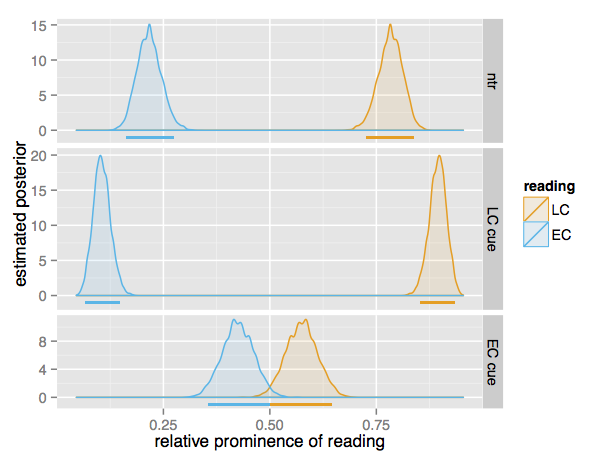
\includegraphics[width=0.8\textwidth]{pics/post_salience_TF_small.png}
  \caption{Estimated posteriors for the salience of \lc- and
    \ec-readings for different prosodic cues. Lines under curves
    indicate 95\% HDIs (see Footnote~\ref{fn:HDI}).}
  \label{fig:Posterior_TF}
\end{figure}
%
Estimates for the (marginalized) posteriors over relative salience
levels for target-related controls are plotted in
Figure~\ref{fig:Posterior_TF}. The results are exactly as we would
expect them to be. Given our data, we should believe that the
\lc-reading is most prominent. The level of prominence varies with
accentuation. Under prosody that we hypothesized would favor the
\lc-reading, the contrast is most pronounced. Under accentuation that
we hypothesized favors the \ec-reading we are no longer justified in
believing with certainty that the \lc-reading is preferred (by
comparison of 95\% HDIs, see below).\footnote{\label{fn:HDI} A 95\%
  Highest Density Interval (HDI) is a convex region of values over
  which 95\% of the distribution's probability density is distributed,
  such that no value outside of that region has higher probability
  density than any point within
  \citep{Kruschke2011:Doing-Bayesian-}. Intuitively speaking, the 95\%
  HDI is the set of values which we may believe to be true with some
  confidence; what falls outside this region is what can be excluded
  safely.}

\begin{figure}
  \centering
  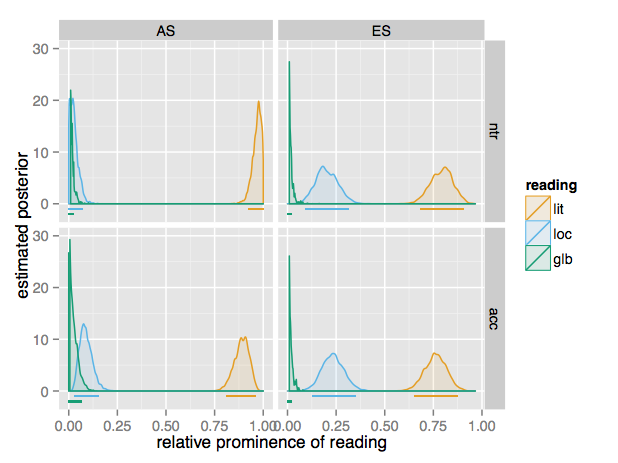
\includegraphics[width=0.8\textwidth]{pics/post_salience_small.png}
  \caption{Posteriors over relative salience of target readings in
    critical conditions.}
  \label{fig:Posterior_T}
\end{figure}

Estimates of posteriors over salience of readings in the critical
conditions are given in Figure~\ref{fig:Posterior_T}. In the
\es-conditions, literal readings are by far the most salient, followed
by local, followed by global readings. There does not appear to be a
significant effect of prosody (by visual comparison of 95\%
HDIs). For \as-sentences, the same preference order holds in tendency,
but we cannot assert with full confidence that local readings are
attested or that they are preferred over global readings (see below).
 
Posteriors over error rates are conceptually less interesting, and we
will skip them here. The posterior over the sequential bias parameter
is shown in Figure~\ref{fig:post_q}. Since the 95\% is clearly
entirely below .5, we have reason for believing, given the model and
our data, in a bias for late responses.

\begin{figure}
  \centering
  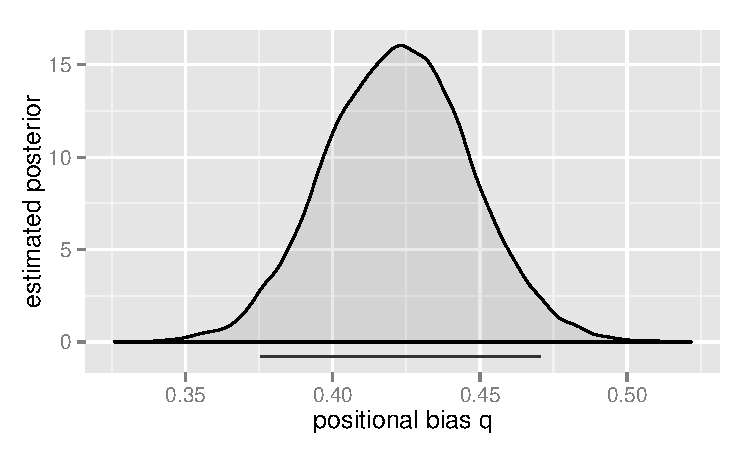
\includegraphics[width=0.5\textwidth]{pics/post_q.pdf}
  \caption{Estimated Posteriors over global sequential bias parameter
    $q$.}
  \label{fig:post_q}
\end{figure}

\paragraph{Model validation.} As a crude sanity check that our model
is able to predict the observed data, we gathered 10.000 random values
from the posterior predictive distribution and found a highly
significant correlation between these and the observed data ($R^2 =
0.987$, $p < 0.001$).

\paragraph{Hypothesis testing.} We are chiefly interested in two
questions: (i) which readings are available? and (ii) what is the
preference order over readings?

The first question can be answered by looking at the HDIs of the
posteriors of the candidate readings. We would like to check the
hypothesis that a given reading is unavailable, i.e., its activation
value in the probabilistic model is equal to 0, or close to zero for
practical purposes (Region of Practical Equivalence, ROPE). We reject
the ``null-hypothesis'' that the true value is 0 if its ROPE lies
entirely outside the 95\% HDI; we accept the ``null-hypothesis'' if
the ROPE lies entirely within the 95\% HDI
\citep[][Ch.~12]{Kruschke2011:Doing-Bayesian-}. The following table
lists approximations of the 95\% HDIs for each condition and reading:

\begin{center}
  \begin{tabular}{lllllll}
    & lit & loc & glb & \\ \midrule
    \as-ntr & $(0.924 , 1)$ & $(0 , 0.068)$
    & $(0 , 0.022)$ \\
    \as-acc 
    & $(0.816 , 0.964)$
    & $(0.028 , 0.152)$
    & $(0 , 0.066)$ \\
    \es-ntr 
    & $(0.665 , 0.873)$
    & $(0.117 , 0.323)$
    & $(0 , 0.024)$ \\
    \es-acc 
    & $(0.634 , 0.851)$
    & $(0.139 , 0.356)$
    & $(0 , 0.022)$ 
  \end{tabular}
\end{center}

\noindent We should thus accept the hypothesis that there are no
global readings at all, and no local readings for \as-sentence under
neutral prosody. There is support for a belief in local readings in
the \as-acc condition up to a ROPE of $[0;0.028)$.

The preference relations between readings can be checked in a similar
way. We look at the posterior beliefs about the \emph{differences} of
activation strengths and ask whether these posterior beliefs allow us
to safely conclude that differences are bigger than zero or not. It is
obvious enough that literal readings are always the most preferred,
and that local readings are preferred over global readings for
\es-sentences. Figure~\ref{fig:PostDiffTAS} shows the posteriors over
differences for the only non-trivial cases, namely those between local
and global readings for \as-sentences. Since the 95\% HDIs include 0,
the data provides no ground for confidence that, given the model,
local readings of \as-sentences are preferred over global ones,
despite the obvious tendency. In sum, with the exception of remaining
uncertainty about local readings of \as-sentences, the model and the
data suggest that global readings are absent entirely, while literal
readings are preferred over local readings.

\begin{figure}
  \centering
  \subfloat[][neutral]{
      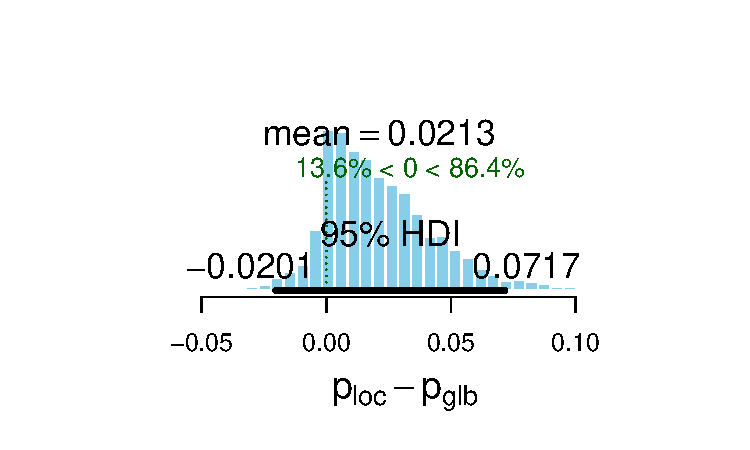
\includegraphics[width=0.45\textwidth]{pics/PostDiffT_ASntr.pdf}
  }
  \hfill
  \subfloat[][accented]{
      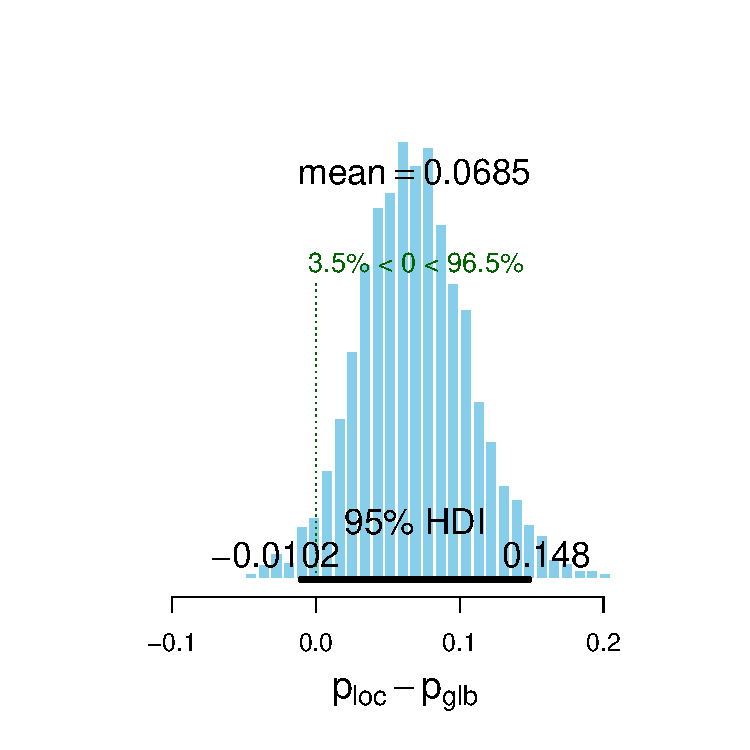
\includegraphics[width=0.45\textwidth]{pics/PostDiffT_ASacc.pdf}
  }
  \caption{Posteriors over differences between salience levels for
    local and global readings of \as-sentences. As zero is contained
    in the 95\% HDI for both neutral and accented variants, there is
    no justification for assuming a difference in salience.}
  \label{fig:PostDiffTAS}
\end{figure}

\subsection{Discussion}
\label{sec:discussion-1}

\paragraph{Summary \& Interpretation.} % The present study investigated
% prosodic effects on quantifier interpretation by employing a new
% experimental paradigm, the incremental verification task. We were
% specifically interested in whether ``local readings'' of sentences
% where \emph{some} is embedded under another quantifier can be found,
% and how salient these readings are under varying prosody of auditorily
% presented sentence material, in particular the presence or absence of
% contrastive stress on embedded \emph{some}.
%
High scores of success in control conditions show that participants
understood the incremental verification task and were able to give
judgements at the right point in a picture sequence. Results for the
preference-related controls show that our design is able to detect
multiple readings and preferences among these. Crucially, the amount
of response types for \lc- and \ec-readings reflected the known
preference for the former, with a mild bias for readings that can be
judged later in the sequence. Also, the incremental verification task
was generally sensitive to prosody. However, our regression analysis
showed that significant prosodic effects were restricted to
preference-related controls. Contrastively, the Bayesian analysis
showed that accenting scalar \emph{some} generally led to more local
readings, but that effect was not significant. Local readings occurred
in \es-sentences, independently of prosody, but required prosodic
marking in \as-sentences. Our analyses support the impression that
inspection of the raw data gives, namely that the general qualitative
pattern of reading preferences is the same for \as- and
\es-conditions: literal readings are preferred over local readings
which are preferred over global readings. More concretely, our
analyses suggest the following preference patterns (bracketed readings
are not supported by our data and the previous analyses):

\begin{exe}
  \ex \label{bsp:observed-preferences}
    \begin{xlist}
      \ex \as-ntr: \ \ \ \lit \ (>  \loc \ \  $\sim$ \glb)
      \ex \as-acc: \ \ \ \lit \ > \ \loc \ \ ( $\sim$ \glb)
      \ex \es-ntr: \ \ \ \lit \ > \ \loc \ \ ( > \glb)
      \ex \es-acc: \ \ \ \lit \ > \ \loc \ \ ( > \glb)
    \end{xlist}

\end{exe}

\noindent Let's consider whether traditionalism or grammaticalism are comfortable with these
preference relations.

Traditionalism easily explains the absence of global readings by holding that the extra
assumptions needed to derive global readings (e.g., a speaker competence assumption) are not
available or only allow for epistemically weak implicatures that would show as responses
indicative of literal readings in our task. In support of this view, traditionalists could
argue that the task's rather high processing demands lead to a suppression of global readings,
in line with the findings of \citet{NeysDe-NeysSchaeken2007:When-People-Are} that working
memory load negatively affects the number of scalar implicature responses in sentence
verification tasks. The finding of local readings in \as-sentences with contrastive stress is
easily explained by adopting the prosodic markedness hypothesis. What traditionalism does not
predict is the high number of answers indicative of local readings in the
\es-conditions. Resorting to the prosodic markedness hypothesis does not help, because local
readings were observed for accented as well as for unaccented \es-sentences.

Grammaticalism, on the other hand, fails to predict the pattern in
(\ref{bsp:observed-preferences}) entirely if it equates preference for readings with logical
strength. Strength-based disambiguation predicts that literal readings of \as-sentences are the
least preferred, contrary to (\ref{bsp:observed-preferences}). Again, we need to bear the
caveat of Section~\ref{sec:grammaticalism} in mind that we are only evaluating grammaticalism
with respect to a particular disambiguation criterion here. The verdict, however, seems to be
clear. If (\ref{bsp:observed-preferences}) shows the actual preference orders over readings,
then meaning disambiguation in terms of logical strength is generally on the wrong track,
because no account that merely looks at the logical strengths of readings can plausibly predict
the preference pattern in (\ref{bsp:observed-preferences}) for both \as- and \es-sentences at
the same time.

In sum, the present findings appear to challenge traditionalism as a ``core theory'', and to
challenge grammaticalism under the ``auxiliary assumption'' that reading preferences mirror
logical strength. Given this, we should ask what plausible amendements or alternative auxiliary
assumptions would enable either position to accommodate the data \emph{ex post}. This is what
we do in the next section, where we also reflect critically on our design and our
interpretation of the data.

\section{Reflection}
\label{sec:critical-reflection}

\subsection{Alternative explanations within the core theories}

Section~\ref{sec:theories-predictions} introduced traditionalism and grammaticalism as two
competing core theories, whose concrete empirical predictions depend on additional
assumptions. Here, we should finally ask more generally: on the supposition that our design and
the offered interpretation of our data are sound, what would it take to accommodate the
observed data under the core theories?

\paragraph{Grammaticalism.} Consider grammaticalism first. Our data contradicts the notion that
preferences follow logical strength. But, as noted in Section~\ref{sec:theories-predictions},
grammaticalism could be supplemented by a conceptually different disambiguation
criterion.\footnote{See also the discussion by \citet{ChemlaSpector2010:Experimental-Ev} on the
  prospects of pushing strength-based disambiguation in the light of their data, which they
  also take to imply contradicting evidence on reading preferences.} Selecting readings in
terms of how well they answer the contextually given question under discussion, as suggested by
\citet{Fox2007:Free-Choice-and,GualminiHulsey2008:The-Question-An}, is an option. But it is
quite unclear what the question under discussion should be that guided judgements in our
particular task. 

Another possibility of explaining our data within a grammaticalist core theory
is to adopt \citeauthor{Magri2011:Another-Argumen}'s (\citeyear{Magri2011:Another-Argumen})
proposal that exhaustification operators occur at every relevant scope site while alternative
sets as their input may also be empty.\footnote{This interesting line of alternative \emph{post
    hoc} explanation was first suggest by a reviewer, but worked out slightly differently here
  to strengthen the reviewer's case.} For \as- and \es-sentences, we would have to consider the
parses in (\ref{Magri-Parses}) (in simplified notation).

\begin{exe}
  \ex \label{Magri-Parses}
    \begin{xlist}
    \ex \label{Magri-Parse-AS} \mymark{$\exh_{Alt_1}$}(\mymark{All} $x$ are such that \mymark{$\exh_{Alt_2}$}( $x$ is connected to
      \mymark{some}  \dots.))
    \ex \label{Magri-Parse-ES} \mymark{$\exh_{Alt_1}$}(\mymark{Exactly
        one} $x$  is such that \mymark{$\exh_{Alt_2}$}( $x$ is connected to \mymark{some}  \dots.))
    \end{xlist}
\end{exe}

\noindent The alternative sets $Alt_{1,2}$ are plausibly either both
empty or both non-empty. In the former case, we get the literal
reading. In the latter case, we should assume that alternatives are
just the standard ones that asymmetrically entail the literal reading:

\begin{exe}
  \ex \label{Magri-Alternatives} 
    \begin{xlist}
    \ex \label{Magri-Alternatives-AS} For \as-sentences: \\
      $Alt_1 = \set{\text{``All } x
          \dots x \text{ is connected to all } \dots \text{''}}$ \\
        $Alt_2 = \set{\text{``}x \text{ is connected to all } \dots
          \text{''}}$
    \ex \label{Magri-Alternatives-AS} For \es-sentences: \\
      % $Alt_1 = \set{\text{``Exactly 1 } x
      %     \dots x \text{ is connected to all } \dots \text{''}}$ \\
      $Alt_1 = \emptyset$ \\
        $Alt_2 = \set{\text{``}x \text{ is connected to all } \dots \text{''}}$
    \end{xlist}
\end{exe}  

\noindent Notice that $Alt_1$ is empty for \es-sentences if we
restrict attention to the ``global alternatives'' that asymmetrically
entail the to-be-interpreted sentence. Interestingly, the readings
that this approach derives are exactly the literal readings (under
empty alternatives) and the local readings (under non-empty
alternatives). What is left to explain is the preference relation over
these readings. Here, the Magri-style approach could resort to
considerations of \emph{economy}: reasoning with fever alternatives is
easier than reasoning with more alternatives. This would explain the
preference for literal readings and also why local readings are more
strongly attested for \es-sentences.

On conceptual grounds we are very much in favor of a disambiguation criterion in terms of
economy considerations, but whether the particular account sketched here is empirically
successful in other cases as well, must remain to be seen. Two things are worth emphasizing
here nonetheless. Firstly, the sketched account is a plausible \emph{post hoc} explanation. It
was not, at least to our knowledge, a salient possibility before seeing our data set: other
specifications of $Alt_1$ and $Alt_2$ could have been made equally plausible \emph{ex
  ante}. Secondly, what our data refutes is that preferences for readings follow logical
strength. This, therefore, does not jeopardize grammaticalism as a core theory, but merely
calls for theory-internal revision of its disambiguation criterion, ideally alongside more
experimental data.

\paragraph{Traditionalism.} Traditionalism, as we described it in
Section~\ref{sec:theories-predictions}, can also not account for the
observed pattern of results. It has to explain the possibility of
local readings of prosodically unmarked \es-sentences, and, perhaps,
also the large number of local readings in accented \es-sentences
compared to the much lower number in accented \as-sentences. A first
option might be to account for alleged local readings as the result of
some other phenomenon, such as typicality or contrast
\citep{Tielvan-Tiel2012:Embedded-Scalar,GeurtsTielvan-Tiel2013:Embedded-Scalar,Tielvan-Tiel2014:Quantity-Matter}.
Since this ties into a critical reflection on our design, we will
enlarge on the possibility of typicality- and contrast-based effects
in our setting. Eventually, we argue that contrast-effects alone are
unlikely to explain the observed high number of local answers in
\es-sentences, but that a ``modern traditionalist'' explanation of the
answer pattern might be available if we allow for the possibility that
\emph{exactly one} gets an unexpected ``referential interpretation.''

As discussed in Section~\ref{sec:previous-studies},
\citet{Tielvan-Tiel2012:Embedded-Scalar} and
\citet{GeurtsTielvan-Tiel2013:Embedded-Scalar} argue that the
distribution of responses to \as-sentences found by
\citet{CliftonDube2010:Embedded-Implic}, as well as
\citet{ChemlaSpector2010:Experimental-Ev} could be explained by
differences in how \emph{typical} the presented pictures were for an
\as-sentence. Notice that this does not apply in the present situation
where the task is to explain away the local readings of \es-sentences,
for which no alternative explanation in terms of typicality has been
offered. Moreover, to apply typicality-based explanations to the
incremental verification task, one would have to reason about the
typicality of parts of pictures or to figure in subjects' expectations
of pictorial typicality given their uncertainty about parts of the
picture that they have not yet seen. On intuitive grounds, we take
either extension to be implausible. But even if this line of
explanation can be plausibly extended to incrementally revealed
picture verification, it would still be unclear why typicality-effects
should show so strongly in categorical truth-value judgements, and why
there is such a stark contrast between \as- and \es-sentences.

A more promising alternative explanation for data indicative of local
readings of \es-sentences is pursued by
\citet{GeurtsTielvan-Tiel2013:Embedded-Scalar} in response to the data
reported by \citet{ChemlaSpector2010:Experimental-Ev}. The main idea
is that visual contrast between an item that is connected to all, and
one that is connected to only some but not all of the relevant
elements may trigger exceptional local enrichment of \emph{some}. In
support of this idea,
\citeauthor{GeurtsTielvan-Tiel2013:Embedded-Scalar} show that the
strength of agreement to an \es-sentence on a 7-point Likert-scale
depends on how strong the relevant visual contrast is. When an item
with only some connections is presented alongside two universally
connected elements, the mean rate of agreement with a suitable
\es-sentence is significantly higher than when only one universally
connected element is present. So, maybe our \es-sequences similarly
provoked local readings because of an overemphasized visual contrast
between \emph{some but not all} and \emph{all}.

The third step of our \es-sequences in Figure~\ref{fig:exseqES} is a
relevant case of direct contrast between a \emph{some-but-not-all-}
and an \emph{all}-situation, but it is a weak contrast, in the sense
of \citet{GeurtsTielvan-Tiel2013:Embedded-Scalar}, because there is
only one universally connected element. Moreover, our study elicited
categorical truth-value judgements. Unlike in
\citeauthor{ChemlaSpector2010:Experimental-Ev}'s
(\citeyear{ChemlaSpector2010:Experimental-Ev}) and
\citeauthor{GeurtsTielvan-Tiel2013:Embedded-Scalar}'s
(\citeyear{GeurtsTielvan-Tiel2013:Embedded-Scalar}) experiments, we
did not record degrees of agreement with a statement. For a purely
contrast-based explanation to work, it would have to be made plausible
why the (weak) visual contrast in a picture like in
Figure~\ref{fig:exseqES3} alone is enough to overrule a truth-value
judgment so as to contradict the semantic meaning (even when there is
no prosodic markedness to support such a reinterpretation).

On the other hand, there is a conceivable alternative explanation of
the puzzling data for \es-sentences that would also account for the
large and systematic error responses. Recall from
Section~\ref{sec:results} and Table~\ref{tab:count_data_CC} on page
\pageref{tab:count_data_CC} that a surprisingly high number of
\emph{true} answers was given at the second step of the
\es-sequence. This answer type does not correspond to any of the three
candidate readings that the previous literature has focused on. As
suggested earlier, this answer type can be explained under the
assumption that \emph{exactly one} gets a reading similar to
\emph{there is (at least) one}, while the scalar item \emph{some}
would just receive its semantic interpretation. Such a reading of
\emph{exactly one}, although surprising, could actually be supported
by some theories of numerals and modifiers
\citep[e.g.][]{Geurts2006:Take-five,MartyChemla2014:Phantom-reading},
as the outcome of an ``existential closure'' type-shifting rule in the
sense of \citet{Partee1987:Noun-phrase-int} to the effect that
\emph{exactly one} is mapped onto an existential reading of the form
``there is a group with cardinality exactly one.''

What happens if \emph{some} is additionally strengthened in some way
or other under such a reading of \emph{exactly one}? If \emph{some} is
pragmatically strengthened under the scope of \emph{at least one} in a
pure traditionalist manner by adding the negation of a sentence type
\emph{at least one \dots all \dots}, we would expect \emph{true}
judgements at position 3 of the \es-sequence. Although exactly 3
\emph{true} answers occurred there for each neutral and accented
\es-conditions respectively, the main point to notice is that this
construal does not explain \emph{true} judgements at position 5, which
we classified as local responses. These would therefore still seem
indicative of local readings. However, there is a slight variant of
the hypothesized existentially closed reading of \emph{exactly one},
that would explain \emph{true} judgments at position 5. This is a
reading of \emph{exactly one} as ``there is a \emph{unique} group with
cardinality exactly one.''  Although this is admittedly only a vague
sketch of a possible line of explanation, it is not entirely
implausible that such a uniqueness requirement has participants, in a
first step of evaluation, look for a distinguished referent, which
they can find no sooner than on position 5 when the whole picture is
unravelled. The search for uniqueness would result in a witness for
the existential quantifier that appears to take a pragmatically
strengthened reading of \emph{some} into account, but that is not
necessarily a ``local reading'' in the sense of
grammaticalism. Moreover, although not strictly required to explain
the behavioral data, we can furthermore explain how the predicate
\emph{is connected to some if its \dots} can be pragmatically enriched
in the desired fashion, along the lines of a ``modern traditionalist''
account that makes use of interpretive mechanisms originally developed
to account for certain discourse phenomena
\citep[][Chapter~8.4]{Geurts2010:Quantity-Implic}. The listener would
then conclude that the referent in question was not connected to all
of its surrounding elements, because otherwise the speaker would have
attributed that to the now fixed referent in question. This is
parallel, so Geurts suggests, to the reasoning that an utterance of
``Smith met a woman'' implicates that \emph{the woman referred to} was
not Smith's mother and not that Smith didn't meet his mother at all.

To wrap up, we suggested amendements to grammaticalism and
traditionalism that could help either position explain the data we
observed. Whether these suggestions can be vindicated by further
empirical research is a matter that we must leave open. It remains,
however, that our data provides interesting challenges to both
traditionalism and grammaticalism, without necessarily refuting either
core theory as such.


\subsection{Critique}

The foregoing discussion presupposed that the interpretation of our
data, given in Section~\ref{sec:discussion-1}, was sound. But there
are a number of conceivable objections that cast into doubt that our
data suggests the preference relation in
(\ref{bsp:observed-preferences}). We will consider the most pressing
ones in the following.

\paragraph{The ``choose first match'' argument.} It is tempting to
think that participants generally tended to choose the first exit
possible. They might, after all, have simply wanted to save time and
be done with the experiment. We considered this a possible confound
and it is therefore that we included the preference-related
controls. But the objection is already clearly refuted by the data
itself. For it would entail that we should see many more global
readings for \es-sentences, which could be judged before the literal
readings, and also that we should have seen the reverse pattern in the
preference-related controls, where we did observe that the reading
that could be judged \emph{later} attracted comparatively more
responses. 

\paragraph{Incomparability of target conditions and preference-related
  controls.} One could object that it is not feasible to compare
results from the preference-related controls to results from our
target conditions, because the source of different readings is
fundamentally different. In the former we have a syntactic ambiguity,
in the latter a set of putative pragmatic enrichments. The former is a
case of perceived ambiguity (some of our subjects reported this), the
latter arguably is not
\citep[see][]{GeurtsPouscoulous2009:Embedded-Implic}. So perhaps even
if the distribution of responses is indicative of the true preference
patterns in preference-related controls, this would not necessarily
mean that the distribution of responses in target conditions is
indicative of preference relations in the same way.

This objection is very serious. It is amplified by an even more
general worry, raised as a challenge by a reviewer, who intuits that
the incremental verification might altogether be insensitive to scalar
implicatures. According to such a view, it could be that, although
\emph{some} is typically strengthened in non-embedded conditions,
virtually all of our participants would exit at an early position
corresponding to the literal reading in a suitable version of our
\ivt.

To address this worry we ran another stripped-down version of the
\ivt. We recruited 50 subjects via Amazon's Mechanical Turk and paid
them 1 US\$ compensation. Similar to our main experiment, the
post-experiment started with two training trials with unambiguous
sentences, familiarizing our subjects with the task. In the
browser-based version, alert boxes pointed out subjects' mistakes when
they tried to exit too early, chose the wrong response or tried to
unravel the sequence further than strictly necessary. The main part of
the experiment consisted of six trials, two of which were critical and
four of which were controls. On critical trials, each subject saw
different version of sentences like (\ref{bsp:Item-PostExp}), in
connection with sequences like in Figure~\ref{fig:Trial-PostExp}.

\begin{exe}
  \ex \label{bsp:Item-PostExp} The scissors are connected to some of the circles.
\end{exe}

\begin{figure}[t]
	\centering
	\subfloat[][Step 2  (\lit true)]{ 
		\fbox{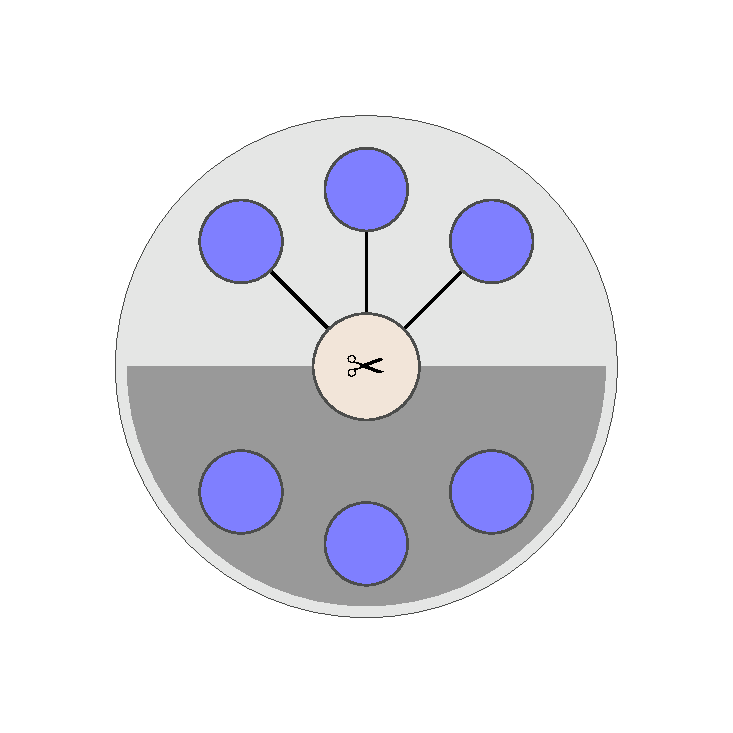
\includegraphics[width=3.5cm]{pictures/PostExp_2.pdf}}
	    \label{fig:exseqPost1}
	}
	\subfloat[][Step 3]{
		\fbox{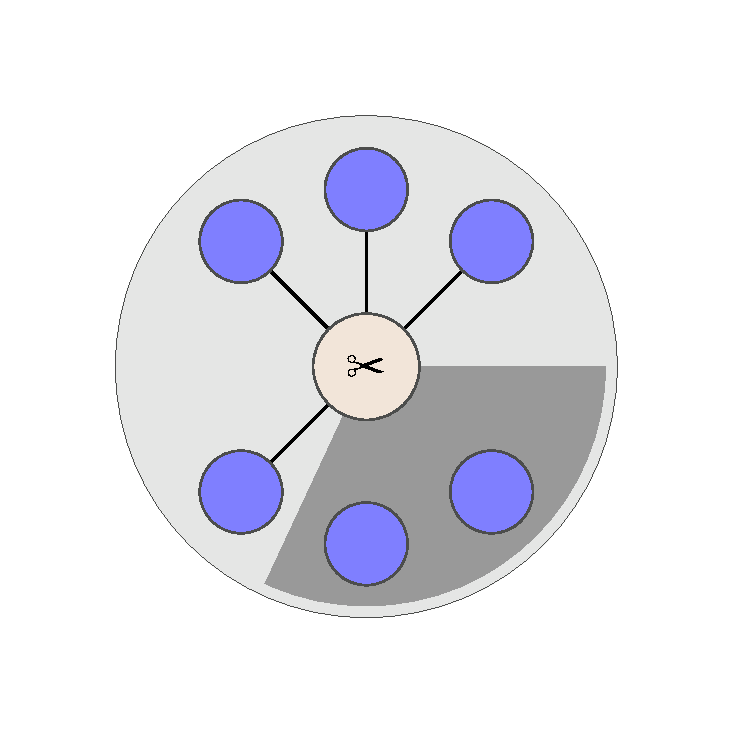
\includegraphics[width=3.5cm]{pictures/PostExp_3.pdf}}
	    \label{fig:exseqPost2}
	}
	\subfloat[][Step 4 (\acro{prag} false)]{ 
		\fbox{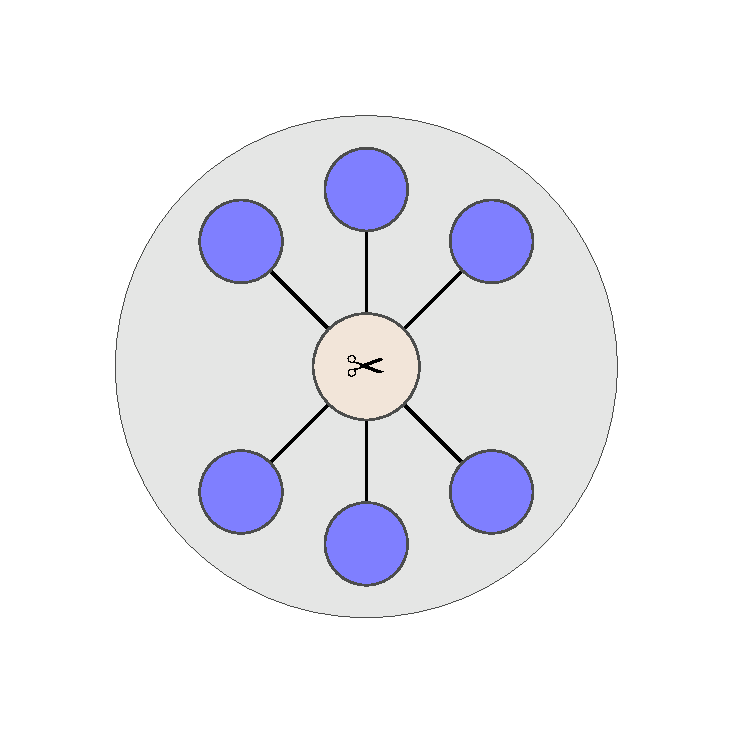
\includegraphics[width=3.5cm]{pictures/PostExp_4.pdf}}
	    \label{fig:exseqPost3}
	}
	\caption{Example sequence for critical trial in
          post-experiment.}
	\label{fig:Trial-PostExp}
\end{figure}

\noindent The first step in the sequence had all potential connections
covered, as before. On step 2, the critical sentence could be judged
true under a literal reading. On the last step 4, it could be judged
false under a pragmatically strengthened implicature reading. Control
conditions had unambiguous sentences and served to filter out subjects
with insufficient performance. From the total of 100 critical trials
(50 subjects times 2 trials each), 66 were literal answers, 27 were
pragmatic answers and 7 were `errors'. If we restrict attention to
only those participants that had at least two of the four control
conditions correct, we are left with 39 subjects. With these, we find
55 literal, 21 pragmatic and 2 `error' answers. In sum, this strongly
suggests that the \ivt is not generally insensitive to scalar
implicature and does give substantial counts also for implicature
readings if these can be judged later than a literal reading. 

If we accept that the \ivt is sensitive to implicature-based
ambiguities, what is left to worry about is that information about
response biases (early vs.~late) do not carry over from the
preference-related control conditions to the target conditions in the
main experiment. It could be, after all, that the task triggers
subjects to exit late for perceived syntactic ambiguities and to exit
early for ``pragmatic ambiguities'' involving implicature
readings. But none of this has any serious impact on the suggested
preference relation in (\ref{bsp:observed-preferences}). For even if
there is a sequential bias in the target conditions to exit early, the
main effect of such a bias would merely be that we should consider
local readings more salient than we do now. In the light of the data
from main and post-experiments, it would be far-fetched to uphold that
our data indicates that local readings are at least as salient as
literal ones. But that means that the suggested interpretation in
(\ref{bsp:observed-preferences}) still holds, and all the problems
that we identified for (the considered versions of) traditionalism and
grammaticalism apply.

% To strengthen this case further, let us assume that the \ivt is
% entirely incapable of reliably indicating preferences among candidate
% pragmatic enrichments of the relevant kind. Can we still draw any
% conclusions about mere availability (non-negligible salience) of
% readings? At a minimum, we would like to uphold that local readings
% are available in \es-sentences and that global readings are unattested
% in \as- and \es-sentences. But that alone is not predicted by either
% traditionalism or grammaticalism in the guises that we considered. The
% former cannot explain the substantial number of local responses in
% \es-sentences, the latter does not explain the total absence of global
% responses.

\paragraph{Interpretation of ``salience'' \& the Bayesian model.}
Another line of criticism that challenges the validity of
(\ref{bsp:observed-preferences}) targets the Bayesian
salience-competition model that we used to derive it. To avoid a
potential misunderstanding pointed out by a reviewer, it is not the
case the our interpretation of the \ivt assumes that each subject
fixes an interpretation at the beginning of the sequence and applies
it, unswayed by anything that is encountered along the sequence of
revealed pictures. The Bayesian model is compatible with this
interpretation, but it is also compatible with a another one that we
think is more plausible, namely that at each choice point during the
sequence of pictures, subjects' aggregate probabilistic behavior is
described as a function that compares the relative salience of the
readings available, together with potential response biases and
uniform error rates. 

Still, we readily admit that our model is highly simplistic. Several
aspects are especially noteworthy here. Firstly, we did not
distinguish different types of errors, and did not take into account
that when errors occurred earlier in the sequence, later decision
points could no longer be reached. This way the model may actually
have unduly de-emphasized the salience of readings that can be judged
later in a sequence. Another, more complicated model of the likelihood
of answer patterns, might therefore have given support to
quantitatively different conclusions. Unfortunately, it is not clear
how exactly such a more complex generating model should be
set-up. Eventually, a full processing model, designed for data from
incremental verification tasks, would be needed. We cannot offer such
a model here, but can only offer a first step in that
direction. More importantly, though, the only part of
(\ref{bsp:observed-preferences}) that might plausibly change for a
more encompassing model along the lines sketched above is that the 3
\emph{false} answers in the \as-conditions with neutral prosody
might support the conclusion that the local reading is attested. But
this hypothetical effect will certainly be no bigger than marginal,
and so no genuinely different conclusions of theoretical relevance
should be expected.

\section{Conclusions}
\label{sec:conclusions}

We tested experimentally the predictions of suitably constrained
versions of traditionalism and grammaticalism with respect to the
availability of and preferences over three types of conceivable
pragmatic enrichments of two types of sentences, in which scalar
\emph{some} occurred in the scope of either the monotonic quantifier
\emph{all} or the non-monotonic quantifier \emph{exactly one}. To
avoid potential confounds of the pictorial material, such as through
typicality or contrast
\citep{Tielvan-Tiel2012:Embedded-Scalar,GeurtsTielvan-Tiel2013:Embedded-Scalar},
we employed an incremental verification task \citep{Conroy2008}, in
which subjects were presented with partially covered pictures and
asked to uncover the picture sequentially until they felt able to give
a categorical truth-value judgements. In order to control for
potential confounds of ``silent prosody,'' sentence material was
presented auditorily and contrastive stress on embedded \emph{some}
was manipulated. This way we were able to also explicitly test the
prosodic markedness hypothesis, which is often used to supplement
traditionalism. Additionally, we included preference-related control
conditions in order to be able to deduce latent preferences for
candidate readings from the answer patterns we gathered. To this end,
we introduced a generative Bayesian model that gives probabilistic
predictions about observable answer patterns in our task, given
concrete instances of relative saliences of readings and other
parameters. Using the observed data, in particular in connection with
the preference-related control conditions, we inferred a posteriori
likely values of the latent model parameters.

Backed up by our analyses, we concluded that both traditionalism and grammaticalism do not
predict our data under the set of auxiliary assumptions that we provided them with in
Section~\ref{sec:theories-predictions}. Traditionalism fails, as a core theory, to account for
high numbers of responses indicating local readings even for prosodically unmarked
\es-sentences. Grammaticalism as a core theory is trivially compatible with our data, because
it would be compatible with any observed preference order. But insofar as it builds on
disambiguation by logical strength, grammaticalism fails to predict the absence of answers
indicative of global readings and the relative abundance of answers indicative of literal
readings.

The clearest upshot of theoretical importance of this study is that strength-based meaning
selection does not seem to be a good disambiguation criterion for grammaticalism
\citep[c.f.][]{ChemlaSpector2010:Experimental-Ev}. This point is also relevant in general,
because disambiguation based on logical strength has been suggested in other domains as well
\citep[e.g.][]{DalrympleKanazawa1998:Reciprocal-Expr,Winter2001:Plural-Predicat,CobrerosEgre2012:Tolerant-Classi}.
We tentatively suggested an alternative selection principle for grammaticalism in terms of
``parsing economy,'' but it remains to be seen whether this is empirically successful in other
domains as well.

Another important conclusion from our data is that \es-sentences,
using non-monotonic quantifier \emph{exactly one}, appeared to be
prone to receive an unexpected interpretation. This may be used by
traditionalism to explain answers indicative of local readings for
\es-sentences. But the point is relevant in general. The possibility
of unexpected interpretations of non-monotonic quantifiers should be
considered also when interpreting the results of other experimental
designs \citep[e.g.][]{CliftonDube2010:Embedded-Implic,
  ChemlaSpector2010:Experimental-Ev}.

We have argued that auditory presentation of sentence material is crucial if prosodic
information is hypothesized to influence availability and preferences of readings. We also
argued in passing that theoretical positions must be formulated in such a way that they make
testable predictions about reading preferences where different potential readings are
allowed. We should then try to obtain information about actual preference patterns by explicit
comparison with constructions whose preference structures are well-studied, ideally with some
model of the data generating process for optimal data analysis.

\newpage

\appendix

\section{The auditory sentence material}
\label{sec:audit-sent-mater}


\begin{table}[!hp]
  \centering
  
  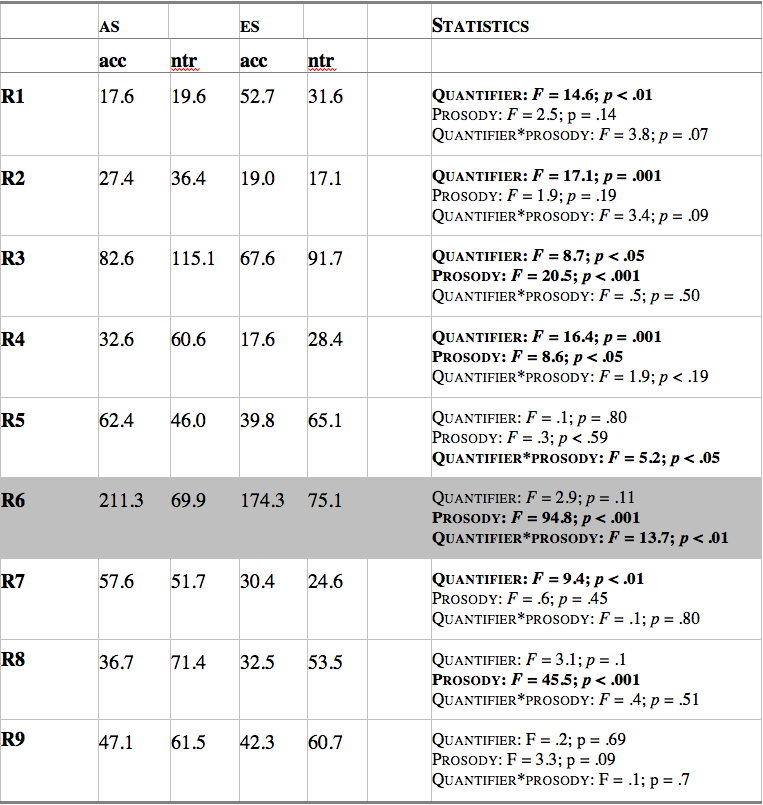
\includegraphics[width=\textwidth]{pictures/Acoustics/Table-B.png}

  \caption{Difference between minimal and maximal F0 values in Hz for
    each of the single words in the target sentences. Region 6
    corresponds to the determiner \emph{einigen}.} 
  \label{tab:table-B}
\end{table}


\begin{table}[!hp]
  \centering
  
  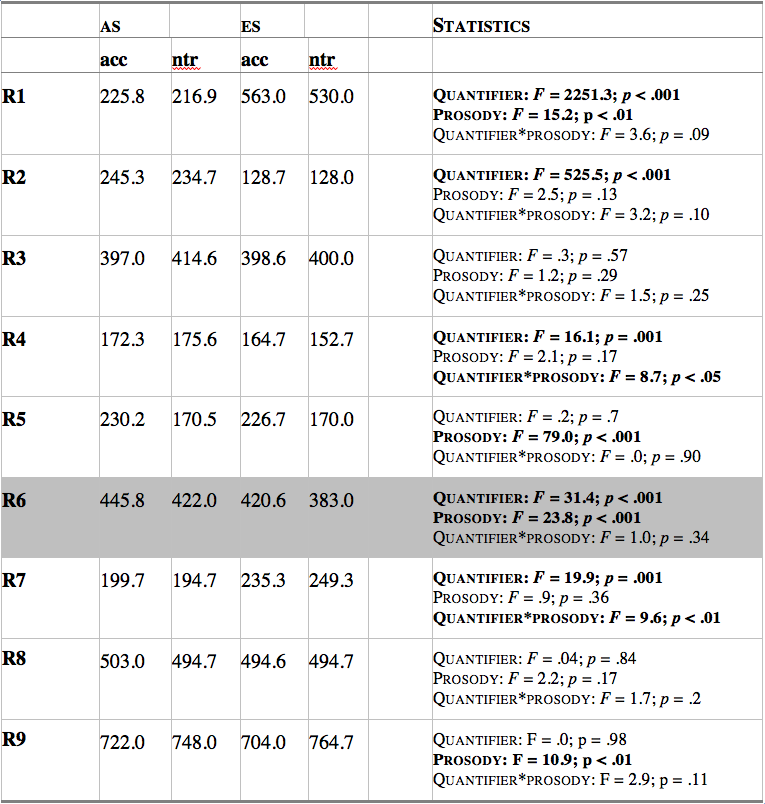
\includegraphics[width=\textwidth]{pictures/Acoustics/Table-A.png}

  \caption{Durational values in ms for each of the single regions in the target sentences. 
  Region 6 corresponds to the determiner \emph{einigen}.}
  \label{tab:table-A}
\end{table}


\begin{table}[hp]
  \centering
  
  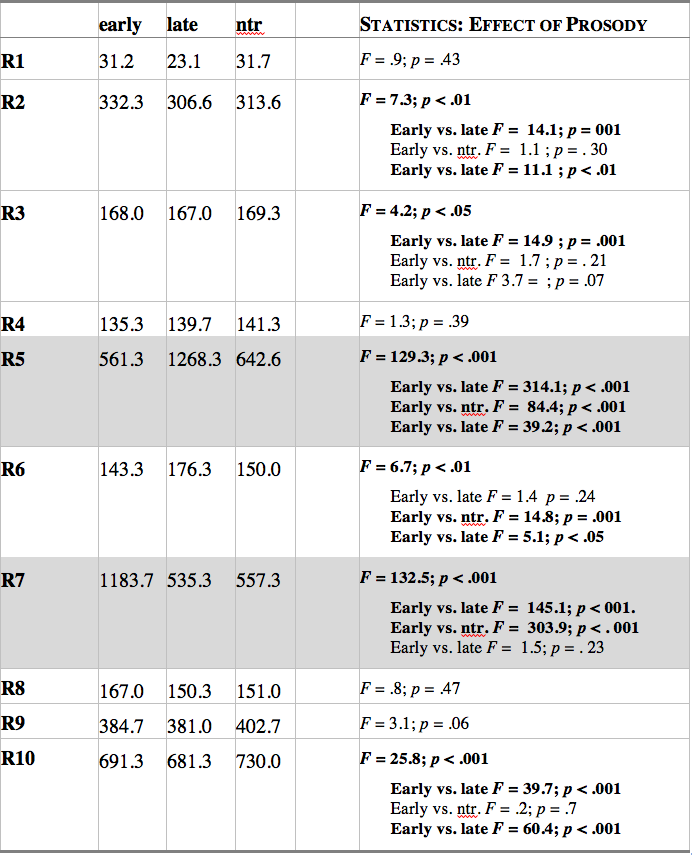
\includegraphics[width=\textwidth]{pictures/Acoustics/Table-D.png}

  \caption{Difference between minimal and maximal F0 values in Hz  
  for each of the single regions in
    the preference-related controls. Regions 5 and 7 correspond to the
    nouns preceding the boundaries.}  
  \label{tab:table-D}
\end{table}


\begin{table}[hp]
  \centering
  
  \includegraphics[width=\textwidth]{pictures/Acoustics/Table-C.png}

  \caption{Durational values in ms for each of the single regions in
    the preference-related controls. Regions 5 and 7 correspond to the
    nouns preceding the boundaries.}  
  \label{tab:table-C}
\end{table}


%\paragraph{Targets.} Table~\ref{tab:table-A} shows the durational values for each of
%the single regions in the sentence. Crucially, durational values of
%accented determiners were significantly increased as opposed to their
%non-accented counterparts. Overall, \acro{Quantifier} effects were
%observed, which might be attributed to the above-mentioned lexical
%differences, as well as to the fact that \es-structures generally
%contained fewer words, thus leading to a tendency of a durational
%decrease for each of the single words.
%
%Differences between maximal and minimal F0 values for each of the
%single words in the sentence are depicted in
%Table~\ref{tab:table-B}. As is descriptively evident, accented
%determiners showed a larger F0 range compared to unaccented versions,
%an effect which is confirmed by statistical analyses. An additional
%\acro{Quantifier}*\acro{Prosody} interaction indicates that these
%differences are even more pronounced in the \as-condition. Finally,
%comparable to the durational analyses, \acro{Quantifier} effects were
%observed when conditions exhibited lexical differences.
%
%Finally, differences between maximal and minimal F0 values for each of
%the single words in the sentence are given in
%Table~\ref{tab:table-D}. Again, the most reliable differences occur at
%the boundary regions.

%\paragraph{Preference-related controls.} Table~\ref{tab:table-C} shows the
%durational values of each of the single words in the sentence. As is
%descriptively evident, the largest durational differences were
%realized at the boundary regions (i.e. Region 5 and Region
%7). Interestingly, small differences between conditions also yielded
%significance at other positions, suggesting that our speaker produced
%the different conditions very consistently (i.e., with little
%variance).

\newpage

\printbibliography[heading=bibintoc]

\end{document}
